\documentclass[oneside, 12pt]{book}
\usepackage[a4paper, total={6in, 8in}, margin=1in, lmargin=2in, tmargin=1.35in, bmargin=1.25in,headsep=1in, footskip=1in]{geometry}
\usepackage{graphicx}
\usepackage{multirow}
\usepackage{float}
\usepackage{fancyhdr}
\usepackage{titlesec}
\usepackage{indentfirst}
\usepackage[table,xcdraw]{xcolor}
\usepackage{xcolor, soul}  
\usepackage{pgf}
\usepackage{pgfpages}
\usepackage{enumerate}
\usepackage{hyperref}
\usepackage{pdfpages}
%\usepackage[none]{hyphenat}
\usepackage{amsfonts}
\usepackage{indentfirst}
\renewcommand{\bibname}{References}

\hypersetup{
    colorlinks,
    citecolor=black,
    filecolor=black,
    linkcolor=black,
    urlcolor=black
}

\counterwithin{figure}{section}
\counterwithin{table}{section}

\makeatletter
\renewcommand{\thesection}{\arabic{section}}
\renewcommand{\thesubsection}{\thesection.\arabic{subsection}}
\renewcommand{\thesubsubsection}{\thesubsection.\arabic{subsubsection}}
\makeatother

\renewcommand{\chaptername}{}

\setcounter{tocdepth}{3}
\setcounter{secnumdepth}{3}

\setlength\parindent{0pt}

\title{Black Book}
\author{
  Arvind Sudarshan,
  \and
  Chatane Shree Atul,
  \and
  Eksambekar Yash Sagar,
  \and
  Gadkari Gaurav Sudhir
}

\renewcommand\footrule{\begin{minipage}{1\textwidth}
\hrule width \hsize height 2pt \kern 1mm \hrule width \hsize   
\end{minipage}\par}%
\fancypagestyle{plain}{
	\fancyhead{}
	\fancyhead[C]{\scriptsize DECENTRALIZED AND SECURE VOTING SYSTEM USING BLOCKCHAIN TECHNOLOGY}
	\fancyfoot{}
	\fancyfoot[C]{\small Department of Computer Engineering AISSMS COE, Pune 2022-23}
	\fancyfoot[R]{\thepage}
}

\pgfpagesdeclarelayout{boxed}
{
  \edef\pgfpageoptionborder{0pt}
}
{
  \pgfpagesphysicalpageoptions
  {%
    logical pages=1
  }
  \pgfpageslogicalpageoptions{1}
  {
    border code=\pgfsetlinewidth{1pt}\pgfstroke,%
    border shrink=\pgfpageoptionborder,%
    resized width=.95\pgfphysicalwidth,%
    resized height=.95\pgfphysicalheight,%
    center=\pgfpoint{.5\pgfphysicalwidth}{.5\pgfphysicalheight}%
  }%
}

\pgfpagesuselayout{boxed}
\nofiles
\begin{document}
\pagestyle{plain}
\renewcommand{\headrulewidth}{0pt}
\titleformat{\chapter}[display]{\bfseries\centering}{\chaptertitlename}{20pt}{\Large\uppercase}

\frontmatter

\begin{titlepage}
	\newgeometry{left=2in,top=0.5in}
	\centering
	\begin{figure}[H]
		\centering
		
\includegraphics[width=0.4\linewidth]{./Resources/sppu.png}
	\end{figure}
	\textbf{SAVITRIBAI PHULE PUNE UNIVERSITY}\break
	\\\textbf{A PRELIMINARY PROJECT REPORT ON}\break
	\\{\large\textbf{DECENTRALIZED AND SECURE VOTING SYSTEM USING BLOCKCHAIN TECHNOLOGY}}\break
	\\SUBMITTED TO THE SAVITRIBAI PHULE PUNE UNIVERSITY, PUNE IN THE PARTIAL FULFILLMENT OF THE REQUIREMENTS FOR THE AWARD OF THE DEGREE\break
	\\OF\break
	\\{\large\textbf{BACHELOR OF ENGINEERING\\(COMPUTER ENGINEERING)}}\break
	\\BY\break
	\begin{table}[H]
		\centering
		\begin{tabular}{lr}
			ARVIND SUDARSHAN      & SEAT NO: B190214209 \\
			CHATANE SHREE ATUL    & SEAT NO: B190214228 \\
			EKSAMBEKAR YASH SAGAR & SEAT NO: B190214241 \\
			GADKARI GAURAV SUDHIR & SEAT NO: B190214244
		\end{tabular}
	\end{table}
	Under the guidance of\break
	\\\textbf{Ms. Snehal S. Kolte}\break
	\begin{figure}[H]
		\centering
		
\includegraphics[width=\linewidth]{./Resources/letterhead2.png}
	\end{figure}
	No. 1, Kennedy Road, Near RTO Office Sangamvadi, Shivajinagar,\\Pune - 411001
	\\\textbf{\large 2022-23}
	\restoregeometry
\end{titlepage}

\begin{titlepage}
	{\centering
	\begin{figure}[H]
		\centering
		
\includegraphics[width=\linewidth]{./Resources/letterhead2.png}
	\end{figure}
	{\Large\textbf{CERTIFICATE}}\break
	\\This is to certify that the project report entitles\break
	\\{\large\textbf{“DECENTRALIZED AND SECURE VOTING SYSTEM USING BLOCKCHAIN TECHNOLOGY”}}\break
	\\Submitted by\break
	\begin{table}[H]
		\centering
		\begin{tabular}{lr}
			ARVIND SUDARSHAN      & SEAT NO: B190214209 \\
			CHATANE SHREE ATUL    & SEAT NO: B190214228 \\
			EKSAMBEKAR YASH SAGAR & SEAT NO: B190214241 \\
			GADKARI GAURAV SUDHIR & SEAT NO: B190214244
		\end{tabular}
	\end{table}}
	is a bonafide work carried out by them under the supervision of \break\textbf{Ms. Snehal S. Kolte} and it is approved for the partial fulfillment of the requirement of Savitribai Phule Pune University Pune for the award of the degree of Bachelor of Engineering (Computer Engineering). This project work has not been earlier submitted to any other Institute or University for the award of any degree or diploma for academic year 2022-23.\\\\\\\\\\
	\begin{table}[H]
		\centering
		\begin{tabular*}{\textwidth}{c@{\extracolsep{\fill}}cccc}
			Ms. Snehal S. Kolte		&	& Mrs. V. V. Navale		&	& Dr. S. V. Athawale			\\
			Project Guide			&	& Project Coordinator	&	& H.O.D.						\\
									&	&						&	& Dept. of Computer Engineering	\\\\\\\\\\
			\multicolumn{1}{l}{}	&	&						&	& Dr. D.S. Bormane              \\\cline{1-1} \cline{3-3}
									&	&						&	& Principal                     \\
			Internal Examiner		&	& External Examiner		&	& AISSMS College of Engineering	\\
		\end{tabular*}
	\end{table}
	Place: Pune
	\\Date:
\end{titlepage}

\begin{titlepage}
	\centering
	{\Large PROJECT APPROVAL SHEET}\break
	\\A\break
	\\Project\break
	\\on\break
	\\{\large\textbf{“DECENTRALIZED AND SECURE VOTING SYSTEM USING BLOCKCHAIN TECHNOLOGY”}}\break
	\\is successfully completed by\break
	\begin{table}[H]
		\centering
		\begin{tabular}{lr}
			ARVIND SUDARSHAN      & SEAT NO: B190214209 \\
			CHATANE SHREE ATUL    & SEAT NO: B190214228 \\
			EKSAMBEKAR YASH SAGAR & SEAT NO: B190214241 \\
			GADKARI GAURAV SUDHIR & SEAT NO: B190214244
		\end{tabular}
	\end{table}
	at\break
	\\\textbf{Department of Computer Engineering}
	\\\textbf{AISSMS College of Engineering, Pune}
	\\\textbf{Savitribai Phule Pune University}
	\\\textbf{2022-2023}\break\break\break\break\break\break
	\begin{table}[H]
		\centering
		\begin{tabular*}{\textwidth}{c@{\extracolsep{\fill}}c}
			Ms. Snehal S. Kolte & Dr. S V Athawale                                                                    \\
			Project Guide         & \begin{tabular}[c]{@{}c@{}}H.O.D.\\ Department of Computer Engineering\end{tabular}
		\end{tabular*}
	\end{table}
\end{titlepage}

\chapter*{Acknowledgement}
We would like to extend our sincere gratitude and thanks to our guide \textbf{Ms. Snehal S. Kolte}, for her invaluable guidance and for giving us useful inputs and encouragement time and again, which inspired us to work harder. Due to her forethought, appreciation of the work involved and continuous imparting of useful tips, this report has been successfully completed.
\\\\We are extremely grateful to \textbf{Dr. S V Athawale}, Head of the Department of Computer Engineering, for his encouragement during the course of the project work.
\\\\We also extend our heartfelt gratitude to the staff of the Computer Engineering Department for their cooperation and support.
\\\\We also take this opportunity to thank all our classmates, friends and all those who have directly or indirectly provided their overwhelming support during our project work and the development of this report.\break\break\break\break\break\break\break\break

\begin{flushright}
	Arvind Sudarshan\\
	Chatane Shree Atul\\
	Eksambekar Yash Sagar\\
	Gadkari Gaurav Sudhir
\end{flushright}

\chapter*{Abstract}
Voting in democratic country is a fundamental right granted to every eligible individual by the constitution. Current e-Voting system used isn’t transparent and can be improved in a few aspects. All voting data from Electronic Voting Machines (EVMs) are stored on a central server. This creates a single point of failure which can be exploited and tampered with easily. Such flaws cause mistrust in the electoral process. Blockchain is a shared  immutable ledger that facilitates the process of recording transactions in a network. It is an emerging technology whose full potential is yet to be realized. Blockchain became popular in 2009 when bitcoin was introduced and used as an alternative to tangible currency and has evolved since. It is a reliable system that can be used in various critical industrial applications. Blockchain has potential to improve the voting system to contest transparent and fair voting. Using this modern technology, a voting system can be implemented which provides transparency leading to fairness in the system. Furthermore, this will overcome the current system flaw of having a single point of failure caused by storing data in a centralized server. In addition to this, election results can be declared faster compared to the current system which might take a few days. The proposed system in this paper shows implementation of voting using blockchain technology.\\\\

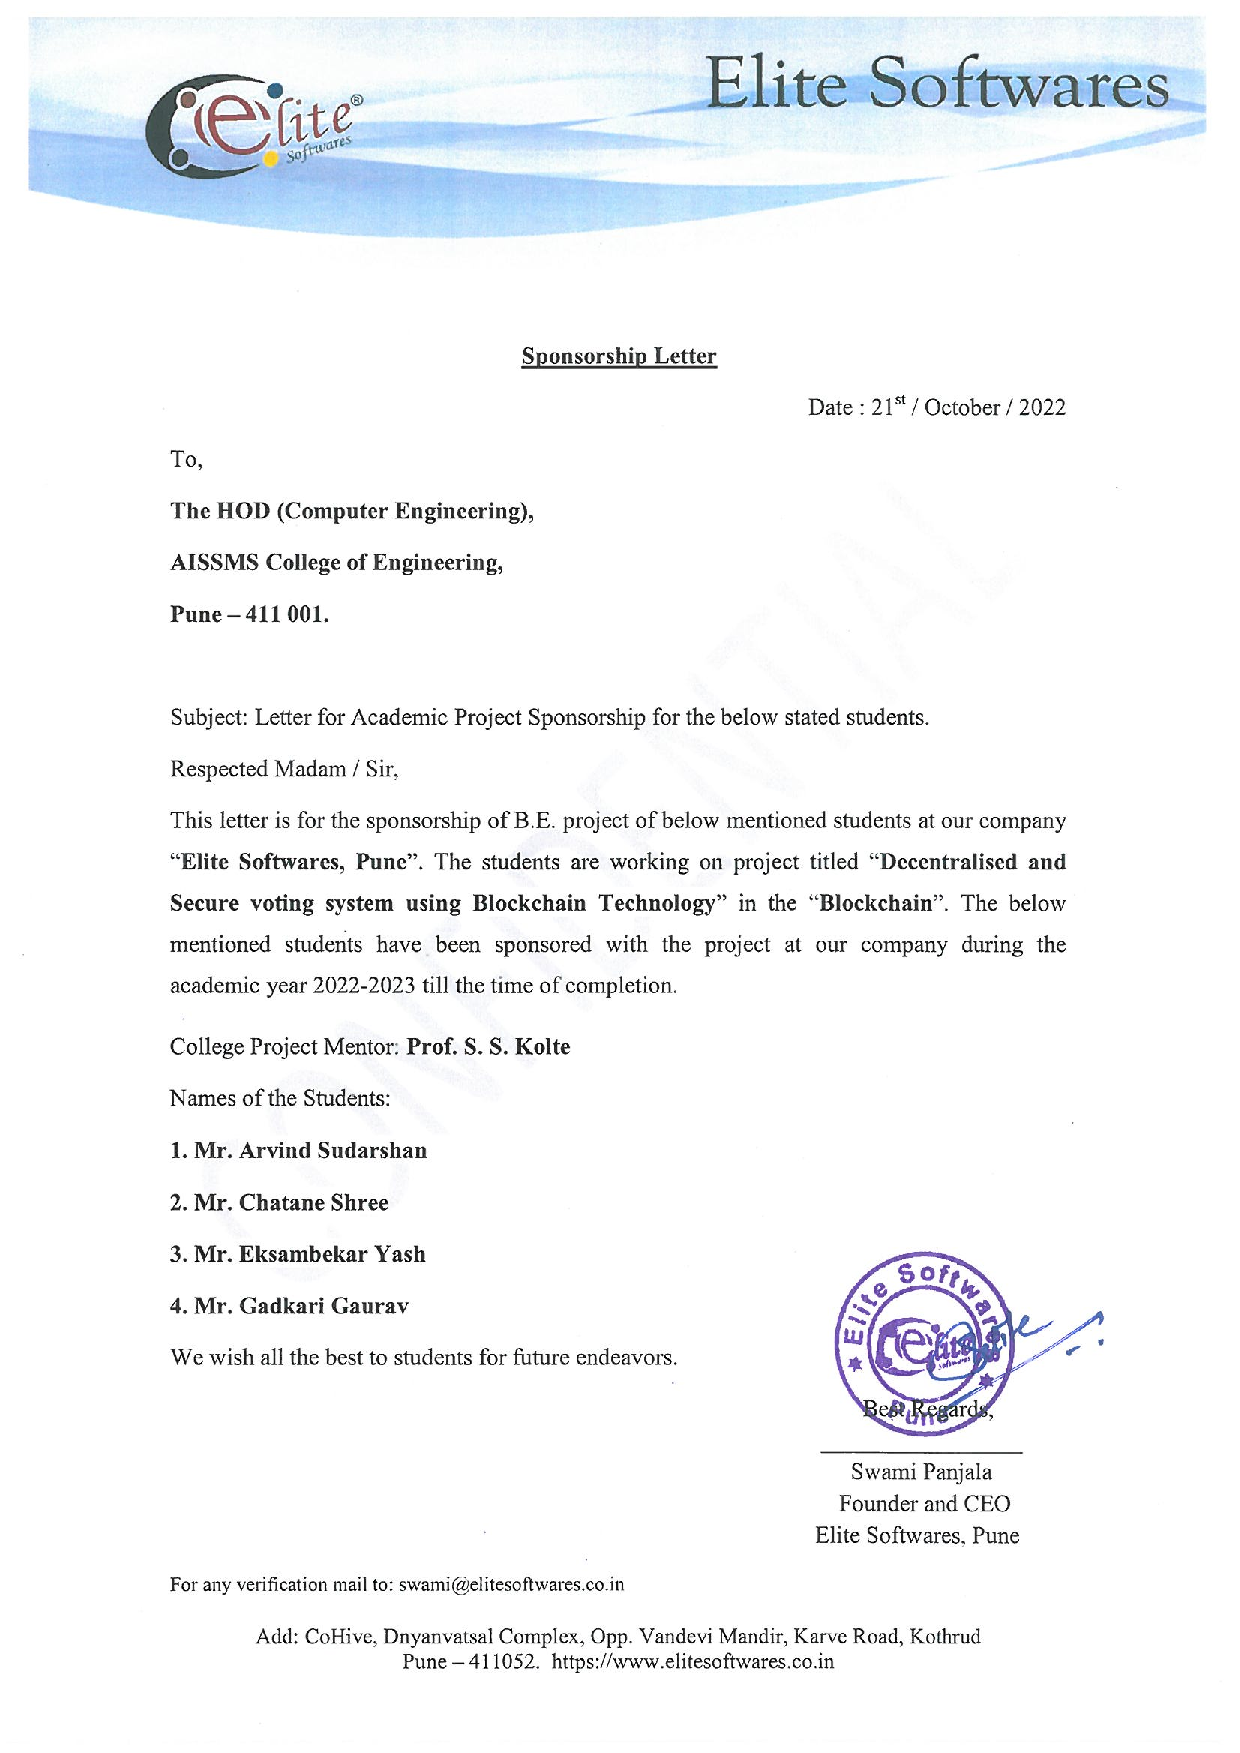
\includepdf[]{./Resources/sponsorship-letter.pdf}

\tableofcontents
\listoffigures
\listoftables

\titleformat{\section}[display]
{\bfseries\centering}
{}
{0.35\textheight}
{\hspace{-0.4pt}\Huge CHAPTER \thesection\\\uppercase}

\mainmatter
\newpage
\section{Synopsis}
\newpage
\subsection{Project Title}
\uppercase{Decentralized and Secure Voting System using Blockchain Technology}
\subsection{Project Option}
Sponsored
\subsection{Internal Guide}
Ms. Snehal S. Kolte
\subsection{Sponsorship and External Guide}
Elite Softwares
\subsection{Problem Statement}
Create a private network responsible for storing and maintaining blockchain. Upon this network, develop a decentralized blockchain based Voting System system based on smart contract which is the optimum solution for frauds, forgery, human error, traceability, stagnancy occurring in the current system providing enhanced security, privacy, efficiency and speed in the voting process.
\subsection{Abstract}
Voting in democratic country is a fundamental right granted to every eligible individual by the constitution. Current e-Voting system used isn’t transparent and can be improved in a few aspects. All voting data from Electronic Voting Machines (EVMs) are stored on a central server. This creates a single point of failure which can be exploited and tampered with easily. Such flaws cause mistrust in the electoral process. Blockchain is a shared  immutable ledger that facilitates the process of recording transactions in a network. It is an emerging technology whose full potential is yet to be realized. Blockchain became popular in 2009 when bitcoin was introduced and used as an alternative to tangible currency and has evolved since. It is a reliable system that can be used in various critical industrial applications. Blockchain has potential to improve the voting system to contest transparent and fair voting. Using this modern technology, a voting system can be implemented which provides transparency leading to fairness in the system. Furthermore, this will overcome the current system flaw of having a single point of failure caused by storing data in a centralized server. In addition to this, election results can be declared faster compared to the current system which might take a few days. The proposed system in this paper shows implementation of voting using blockchain technology.
\subsection{Goals and Objectives}
To design a decentralized e-voting system that,
\begin{enumerate}
	\item Eliminate humans from the process.
	\item Does not depend on a trusted third party for controlling the collected data, whilst still staying immune to attacks and guaranteeing user privacy.
	\item Provides transparency, ensuring security and does not jeopardize voter privacy.
\end{enumerate}
\subsection{Plan of Project Execution}
\begin{table}[H]
	\resizebox{\textwidth}{!}{%
		\begin{tabular}{|l|l|l|l|l|l|l|l|l|l|l|l|l|}
			\hline                                                                 & June                     & July                     & August                   & September                & October                  & November                 & December                 & January                  & February                 & March                    & April                    & May                      \\ \hline
			Project scouting                                                       & \cellcolor[HTML]{FFCB2F} &                          &                          &                          &                          &                          &                          &                          &                          &                          &                          &                          \\ \hline
			Feasibility Study                                                      &                          & \cellcolor[HTML]{FFCB2F} &                          &                          &                          &                          &                          &                          &                          &                          &                          &                          \\ \hline
			Literature Survey                                                      &                          &                          & \cellcolor[HTML]{FFCB2F} & \cellcolor[HTML]{FFCB2F} &                          &                          &                          &                          &                          &                          &                          &                          \\ \hline
			Project definition                                                     &                          &                          &                          & \cellcolor[HTML]{FFCB2F} &                          &                          &                          &                          &                          &                          &                          &                          \\ \hline
			\begin{tabular}[c]{@{}l@{}}Project interface\\ definition\end{tabular} &                          &                          &                          &                          & \cellcolor[HTML]{FFCB2F} &                          &                          &                          &                          &                          &                          &                          \\ \hline
			\begin{tabular}[c]{@{}l@{}}Requirement\\ gathering\end{tabular}        &                          &                          &                          &                          & \cellcolor[HTML]{FFCB2F} &                          &                          &                          &                          &                          &                          &                          \\ \hline
			Documentation                                                          &                          &                          &                          &                          & \cellcolor[HTML]{FFCB2F} & \cellcolor[HTML]{FFCB2F} &                          &                          &                          &                          &                          &                          \\ \hline
			\begin{tabular}[c]{@{}l@{}}Phase 1\\ implementation\end{tabular}       &                          &                          &                          &                          &                          &                          & \cellcolor[HTML]{FFCB2F} & \cellcolor[HTML]{FFCB2F} &                          &                          &                          &                          \\ \hline
			\begin{tabular}[c]{@{}l@{}}Phase 2\\ implementation\end{tabular}       &                          &                          &                          &                          &                          &                          &                          & \cellcolor[HTML]{FFCB2F} & \cellcolor[HTML]{FFCB2F} &                          &                          &                          \\ \hline
			\begin{tabular}[c]{@{}l@{}}Journal paper\\ publication\end{tabular}    &                          &                          &                          &                          &                          &                          &                          &                          & \cellcolor[HTML]{FFCB2F} & \cellcolor[HTML]{FFCB2F} & \cellcolor[HTML]{FFCB2F} &                          \\ \hline
			\begin{tabular}[c]{@{}l@{}}Project report\\ finalizing\end{tabular}    &                          &                          &                          &                          &                          &                          &                          &                          &                          &                          & \cellcolor[HTML]{FFCB2F} & \cellcolor[HTML]{FFCB2F} \\ \hline
			\begin{tabular}[c]{@{}l@{}}Final project\\ implementation\end{tabular} &                          &                          &                          &                          &                          &                          &                          &                          &                          &                          & \cellcolor[HTML]{FFCB2F} & \cellcolor[HTML]{FFCB2F} \\ \hline
		\end{tabular}%
	}
	\caption{Timeline Chart}
	\label{tab:timeline-chart}
\end{table}
\newpage
\section{Technical Keywords}
\newpage
\subsection{Area of Project}
\begin{enumerate}
	\item Blockchain Technology
	\item Secured Voting
\end{enumerate}
\subsection{Technical Keywords}
\begin{enumerate}
	\item Blockchain Technology
	\item Ethereum Virtual Machine
	\item Voting System
	\item Secure Voting
	\item Central Server
	\item Transparency
	\item Single Point of Failure
\end{enumerate}
\newpage
\section{Introduction}
\newpage
\subsection{Overview}
Blockchain technology can be used in the E-voting system to conduct a fair election and reduce injustice. The physical voting systems have many flaws in it as well as the digital voting systems are not perfect enough to be implemented on a large scale. This paper presents an overview of Blockchain based voting systems. The proposed platform will provide a framework that can be implemented to conduct voting activity digitally through blockchain. Our proposed system will use a flexible blockchain with consensus algorithms. The Chain security algorithm used in makes voting transactions more secure and integrated.
\\\textbf{Blockchain:} Blockchain is like a distributed ledger technology consisting of records of transactions called as blocks that are linked together using mathematical cryptography. Blockchain technology is popular because of its distributed nature which makes it immutable and practically impossible to hack.
\\\textbf{Distributed Ledger:} Ledger is a records collection containing information about transactions. Distributed ledger is a data structure capable of storing said transactions which is distributed across different computers on the network. DLT (Distributed Ledger Technology) is technology that distributes transaction records to all the users participating in the network. Blockchain is a type of Distributed Ledger Technology(DLT). Hence the data is shared among all its users providing transparency and preventing corruption.
\\\textbf{Decentralized Application(dApp):} dApp is an application built to run on decentralized computing, blockchain or any other distributed ledger system. It makes use of smart contracts for its functioning.
\\\textbf{Smart Contract:} Smart contracts are computer programs that automatically execute or control actions according to the terms of a contract or an agreement. It is used to enforce rules in blockchain transactions. Smart contracts are considered fundamental building blocks for cryptocurrencies and NFTs.
\\\textbf{Consensus:} Consensus ensures that all the different users participating in blockchain come to a mutual agreement regarding the state of blockchain. There are numerous consensus mechanisms that are used by different blockchain applications.
\\\textbf{Cryptography:} Cryptography is based on mathematical theory and computer science. Cryptography’s importance is to provide methods to secure and protect data and communications using encryption related techniques.
\\\textbf{Ethereum:} Ethereum is an open-source blockchain which provides smart contract functionality using solidity programming language.
\newpage
\subsection{Motivation}
India is said to have the largest democracy. For the electoral voting system India is using modern “Electronic Voting Machines” which are responsible for taking user input and storing the votes entered by the end user. Later these votes are carried to a central location where they are counted and the result is declared. Though, there is a possibility that these votes data can be tampered with. Having a single central server to store data creates a single point of failure for the entire system. These issues cause mistrust regarding the current system. In the traditional ballot paper system, vote authenticity was questionable and had its separate issues for which it was replaced with modern Electronic Voting Machines. Blockchain is based on Distributed Ledger Technology(DLT). In DLT, replicas of the same data are made on different nodes in the network due to which there is no single point of failure. Moreover, due to consensus algorithms implemented in blockchain, all nodes decide and agree upon whether a block is valid and must be added to the network or not.
\\\\Using Blockchain Technology will overcome issues in the present electronic voting system. It will also contribute to increasing the overall trust in the system and benefit democracy. Blockchain will provide a secure system for vote acceptance, storage and provide faster election results.
\subsection{Objective}
To design a decentralized e-voting system that,
\begin{enumerate}
	\item Reduces human interaction in the process of voting and elections in general.
	\item Does not depend on a trusted third party for controlling the collected data, whilst still staying immune to attacks and guaranteeing user privacy.
	\item Provides transparency, ensuring security and does not jeopardize voter privacy.
\end{enumerate}
\newpage
\section{Literature Survey}
\newpage
\subsection{Study of Research Paper}
\begin{enumerate}
	\item
	      \textbf{Paper Name:} Blockchain challenges and opportunities: a survey \cite{zheng2018blockchain}\\
	      \textbf{Authors:} Zibin Zheng, Shaoan Xie, Hong-Ning Dai, Xiangping Chen and Huaimin Wang\\
	      \textbf{Abstract:} Blockchain has numerous benefits such as decentralisation, persistency, anonymity and auditability. There is a wide spectrum of blockchain applications ranging from cryptocurrency, financial services, risk management, internet of things (IoT) to public and social services. Although a number of studies focus on using the blockchain technology in various application aspects, there is no comprehensive survey on the blockchain technology in both technological and application perspectives. To fill this gap, we conduct a comprehensive survey on the blockchain technology. In particular, this paper gives the blockchain taxonomy, introduces typical blockchain consensus algorithms, reviews blockchain applications and discusses technical challenges as well as recent advances in tackling the challenges. Moreover, this paper also points out the future directions in the blockchain technology.\\
	      \textbf{Inference:}
	      \\Blockchain gained most of its fame from bitcoin, a cryptocurrency.
	      \\It is the backbone of bitcoin. The concept of blockchain was introduced in 2008 and implemented a year later. Satoshi Nakamoto is dubbed as the creator of blockchain. Blockchain has several different characteristics like decentralisation, persistence, anonymity and auditability. Blockchain has various diverse applications other than bitcoin.Its ability to conduct transactions without banks make it a strong contender for online payments.
	\item
	      \textbf{Paper Name:} A Survey on Blockchain Technology: Evolution, Architecture and Security \cite{bhutta2021survey}\\
	      \textbf{Authors:} Bhutta, Muhammad Nasir Mumtaz, Amir A. Khwaja, Adnan Nadeem, Hafiz Farooq Ahmad, Muhammad Khurram Khan, Moataz A. Hanif, Houbing Song, Majed Alshamari, and Yue Cao\\
	      \textbf{Abstract:} Blockchain is a revolutionary technology that is making a great impact on modern society due to its transparency, decentralization, and security properties. Blockchain gained considerable attention due to its very first application of Cryptocurrencies e.g., Bitcoin. In the near future, Blockchain technology is determined to transform the way we live, interact, and perform businesses. Recently, academics, industrialists, and researchers are aggressively investigating different aspects of Blockchain as an emerging technology. Unlike other Blockchain surveys focusing on either its applications, challenges, characteristics, or security, we present a comprehensive survey of Blockchain technology's evolution, architecture, development frameworks, and security issues. We also present a comparative analysis of frameworks, classification of consensus algorithms, and analysis of security risks \& cryptographic primitives that have been used in the Blockchain so far. Finally, this paper elaborates on key future directions, novel use cases and open research challenges, which could be explored by researchers to make further advances in this field.\\
	      \textbf{Inference:}
	      \\This paper covers the Blockchain technology’s evolution, its security and architecture.
	      \\Blockchain 1.0 is used in bitcoin founded by anonymous person with pseudoname Satoshi Nakamoto. Cryptocurrencies are the first applications of Blockchain technology and are already functional as a digital payment alternative on the World Wide Web.
	      \\Blockchain 2.0 is based on Smart Contracts. It is used for transferring assets like bonds, stocks, loans, Properties etc. Afterwards it is realised that that Blockchain can revolutionise for all the industries.
	      \\Blockchain 3.0 provides a platform for development of secure applications for all the industries rather than only money exchange. It supports large scale interconnection using web technology.
	\item
	      \textbf{Paper Name:} Blockchain characteristics and consensus in modern business processes \cite{viriyasitavat2019blockchain}\\
	      \textbf{Authors:} Viriyasitavat, Wattana and Danupol Hoonsopon\\
	      \textbf{Abstract:} Blockchain technology has attracted a great deal of attentions as an effective way to innovate business processes. It has to be integrated with other Business Process Management system (BPM) components to implement specified functionalities related to the applications. The current efforts in integrating this technology into BPM are at a very early stage. To apply Blockchain into business processes efficiently, Blockchain and business process characteristics must be identified. Inconsistency of confirmation settlement that heavily relies on the implementation of consensus protocol poses a major challenge in business process operations, especially ones that are time-critical. In addition, validators, nodes responsible for performing consensus operations in a Blockchain system, can introduce bias and as a result are not trustable. This paper first defines Blockchain and also investigates the characteristics of Blockchain and business processes. Then, we suggest an architecture of business processes in Blockchain era to overcome the problems of time inconsistency and consensus bias. The architecture provides persistency, validity, auditability, and disintermediary that Blockchain offers. The architecture also provides flexibility by allowing business partner to select nodes in performing consensus; thus bias is mitigated.\\
		  \newpage
	      \textbf{Inference:}
	      \begin{itemize}
		      \item\textbf{Cost effective:} In traditional systems there is a need of some central organizaion to verify the validity of transactions. Blockchain is a peer to peer network(P2P). The absence of a central agency reduces the cost per transaction.
		      \item\textbf{Persistence:} Blockchain has one important property of persistence, Each block has the ability to maintain its records. This helps in keeping the data tamper proof.
		      \item\textbf{Validity:} The execution is not carried out every time. This system has three roles, proposer, acceptor, learner.
		      \item\textbf{Anonymity \& Identity:} The centralised systems require to know you as a person. You need to register your identity proof with those authorities. Whereas with blockchain, the user data remains fairly anonymous.
		      \item\textbf{Auditability:} The block added to the blockchain remains there forever. This helps in checking transaction history. In private blockchain the auditability is least and depends on the central entity. In permissioned blockchain there is a little bit of auditability. In public blockchain have the most auditability.
	      \end{itemize}
	\item
	      \textbf{Paper Name:} An Overview of Blockchain Technology: Architecture, Consensus, and Future Trends \cite{zheng2017overview}\\
	      \textbf{Authors:} Zheng, Zibin and Xie, Shaoan and Dai, Hong-Ning and Chen, Xiangping and Wang, Huaimin\\
	      \textbf{Abstract:} Blockchain, the foundation of Bitcoin, has received extensive attentions recently. Blockchain serves as an immutable ledger which allows transactions take place in a decentralized manner. Blockchain-based applications are springing up, covering numerous fields including financial services, reputation system and Internet of Things (IoT), and so on. However, there are still many challenges of blockchain technology such as scalability and security problems waiting to be overcome. This paper presents a comprehensive overview on blockchain technology. We provide an overview of blockchain architechture firstly and compare some typical consensus algorithms used in different blockchains. Furthermore, technical challenges and recent advances are briefly listed. We also lay out possible future trends for blockchain.\\
	      \textbf{Inference:}
	      \\In Blockchain Technology, there exists three major types: Privete, Consortium and Public blockchain. Since a network will have to be created, a comparison must be made on what kind of network must be used for the same. The types are compared on the basis of Consensus determination, Read permission, Immutability, Efficiency, whether it is centralised or not and the Consensus process. Depending upon the application, a developer must decide what kind of blockchain should be used. Table \ref{tab:types-of-blockchains} shows a comparision between the types of blockchains.
	      \begin{table}[H]
		      \centering
		      \resizebox{\textwidth}{!}{%
			      \begin{tabular}{|l|lll|}
				      \hline
				      \multicolumn{1}{|c|}{\multirow{2}{*}{\textbf{Property}}} & \multicolumn{3}{c|}{\textbf{Types of Blockchain}}                                                                                     \\ \cline{2-4}
				      \multicolumn{1}{|c|}{}                                   & \multicolumn{1}{l|}{\textbf{Private}}              & \multicolumn{1}{l|}{\textbf{Consortium}}           & \textbf{Public}             \\ \hline
				      Consensus determination                                  & \multicolumn{1}{l|}{Single Organisation}           & \multicolumn{1}{l|}{Selected nodes}                & All participating miners    \\ \hline
				      Read permission                                          & \multicolumn{1}{l|}{Could be public or restricted} & \multicolumn{1}{l|}{Could be public or restricted} & Public                      \\ \hline
				      Immutability                                             & \multicolumn{1}{l|}{Could be tampered}             & \multicolumn{1}{l|}{Could be tampered}             & Nearly impossible to tamper \\ \hline
				      Efficiency                                               & \multicolumn{1}{l|}{High}                          & \multicolumn{1}{l|}{High}                          & Low                         \\ \hline
				      Centralised                                              & \multicolumn{1}{l|}{Yes}                           & \multicolumn{1}{l|}{Partial}                       & No                          \\ \hline
				      Consensus process                                        & \multicolumn{1}{l|}{Permissioned}                  & \multicolumn{1}{l|}{Permissioned}                  & Permissionless              \\ \hline
			      \end{tabular}%
		      }
		      \caption{Types of Blockchains}
		      \label{tab:types-of-blockchains}
	      \end{table}
	\item
	      \textbf{Paper Name:} Comparative analysis of blockchain consensus algorithms \cite{bach2018comparative}\\
	      \textbf{Authors:} L. M. Bach, B. Mihaljevic and M. Zagar\\
	      \textbf{Abstract:} Cryptocurrencies have seen a massive surge in popularity and behind these new virtual currencies is an innovative technology called the blockchain: a distributed digital ledger in which cryptocurrency transactions are recorded after having been verified. The transactions within a ledger are verified by multiple clients or “validators,” within the cryptocurrency's peer-to-peer network using one of many varied consensus algorithms for resolving the problem of reliability in a network involving multiple unreliable nodes. The most widely used consensus algorithms are the Proof of Work (PoW) algorithm and the Proof of Stake (PoS) algorithm; however, there are also other consensus algorithms which utilize alternative implementations of PoW and PoS, as well as other hybrid implementations and some altogether new consensus strategies. In this paper, we perform a comparative analysis of typical consensus algorithms and some of their contemporaries that are currently in use in modern blockchains. Our analysis focuses on the algorithmic steps taken by each consensus algorithm, the scalability of the algorithm, the method the algorithm rewards validators for their time spent verifying blocks, and the security risks present within the algorithm. Finally, we present our conclusion and some possible future trends for consensus algorithms used in blockchains.\\
	      \textbf{Inference:}
	      \\The Oxford Dictionary meaning of word consensus is: an opinion that all members of a group agree with. In Blockchain Technology every transaction must be verified and agreed upon by validators in the network before being inserted. To do so, various consensus algorithms have been defined for use. Few of the most used consensus algorithms are Proof of Stake (PoS) algorithm and Proof of Work (PoW) algorithm.
	      \\In this paper referenced, the authors have mentioned a few of the consensus algorithms used and their comparative analysis. Some High-profile consensus algorithms mentioned in the paper are Proof of Work (PoW), Proof of Stake (PoS), Proof of Importance (PoI), Delegated Proof of Stake (dPOS), Stellar Consensus Protocol (SCP) and Ripple Protocol Consensus Algorithm (RPCA). The authors have compared these algorithms on the basis of Security, Scalability and Power Consumption. A consensus algorithm characteristic comparison is provided in Table \ref{tab:consensus-algorithm-comparision}.
	      \begin{table}[H]
		      \centering
		      \resizebox{\textwidth}{!}{%
			      \begin{tabular}{|l|llllll|}
				      \hline
				      \multicolumn{1}{|c|}{\multirow{2}{*}{\textbf{Property}}}               & \multicolumn{6}{c|}{\textbf{Algorithm Name}}                                                                                                                                                                                                                                                                                                                                                                                                       \\ \cline{2-7}
				      \multicolumn{1}{|c|}{}                                                 & \multicolumn{1}{l|}{\textbf{PoW}}                                                                & \multicolumn{1}{l|}{\textbf{RPCA}}                                                          & \multicolumn{1}{l|}{\textbf{PoS}}          & \multicolumn{1}{l|}{\textbf{SCP}} & \multicolumn{1}{l|}{\textbf{dPOS}}                                                        & \textbf{PoI}                                                         \\ \hline
				      Energy Saving                                                          & \multicolumn{1}{l|}{No}                                                                          & \multicolumn{1}{l|}{Yes}                                                                    & \multicolumn{1}{l|}{Partial}               & \multicolumn{1}{l|}{Yes}          & \multicolumn{1}{l|}{Partial}                                                              & Yes                                                                  \\ \hline
				      \begin{tabular}[c]{@{}l@{}}Tolerated power\\ of adversary\end{tabular} & \multicolumn{1}{l|}{\begin{tabular}[c]{@{}l@{}}\textless{}25\%\\ computing\\ power\end{tabular}} & \multicolumn{1}{l|}{\begin{tabular}[c]{@{}l@{}}\textless{}20\% faulty\\ nodes\end{tabular}} & \multicolumn{1}{l|}{\textless{}51\% stake} & \multicolumn{1}{l|}{Variable}     & \multicolumn{1}{l|}{\begin{tabular}[c]{@{}l@{}}\textless{}51\%\\ validators\end{tabular}} & \begin{tabular}[c]{@{}l@{}}\textless{}50\%\\ importance\end{tabular} \\ \hline
				      Example                                                                & \multicolumn{1}{l|}{Bitcoin}                                                                     & \multicolumn{1}{l|}{Ripple}                                                                 & \multicolumn{1}{l|}{Cardano}               & \multicolumn{1}{l|}{Stellar}      & \multicolumn{1}{l|}{EOS}                                                                  & NEM                                                                  \\ \hline
			      \end{tabular}%
		      }
		      \caption{Consensus Algorithm Comparision}
		      \label{tab:consensus-algorithm-comparision}
	      \end{table}
	\item
	      \textbf{Paper Name:} Solutions to Scalability of Blockchain: A Survey \cite{zhou2020solutions}\\
	      \textbf{Authors:} Q. Zhou, H. Huang, Z. Zheng and J. Bian\\
	      \textbf{Abstract:} Blockchain-based decentralized cryptocurrencies have drawn much attention and been widely-deployed in recent years. Bitcoin, the first application of blockchain, achieves great success and promotes more development in this field. However, Bitcoin encounters performance problems of low throughput and high transaction latency. Other cryptocurrencies based on proof-of-work also inherit the flaws, leading to more concerns about the scalability of blockchain. This paper attempts to cover the existing scaling solutions for blockchain and classify them by level. In addition, we make comparisons between different methods and list some potential directions for solving the scalability problem of blockchain.\\
	      \textbf{Inference:}
	      \begin{itemize}
		      \item\textbf{Bitcoin-Cash:} It is another form of cryptocurrency. It is the hard fork from bitcoin’s codebase. The main idea is to solve the scalability issue of the blockchain. The solution here is to increase the block size while keeping the block interval the same. The block size of bitcoin was 1 MB, but now bitcoin and bitcoin cash has increased its blocksize to 8 MB. After that there was further increase in the block size of bitcoin cash to 32 MB.However we cannot increase the blocksize infinitely as there is a limitation to the intra-blockchain bandwidth. The larger block sizes may also lead to the problems of centralization.
		      \item\textbf{Block compression:} In compact block relay technique the data structure is little altered. The block contains the headers and some short transaction IDs,  used to match transactions already available to the receivers. The compact block messages are sent and receivers process these messages. The node A sends the compact block to the node B. When node B receives the compact block it calculates the transaction IDs in the memory pool and matches it with the transactions IDs in the compact block. If all transactions are available the block is reconstructed if not node B sends the getblocktxn message to node A to receive all transaction data. After that the block is constructed. In low bandwidth relaying the compact blocks are sent only if the request is made.
		      \begin{figure}[H]
			      \centering
			      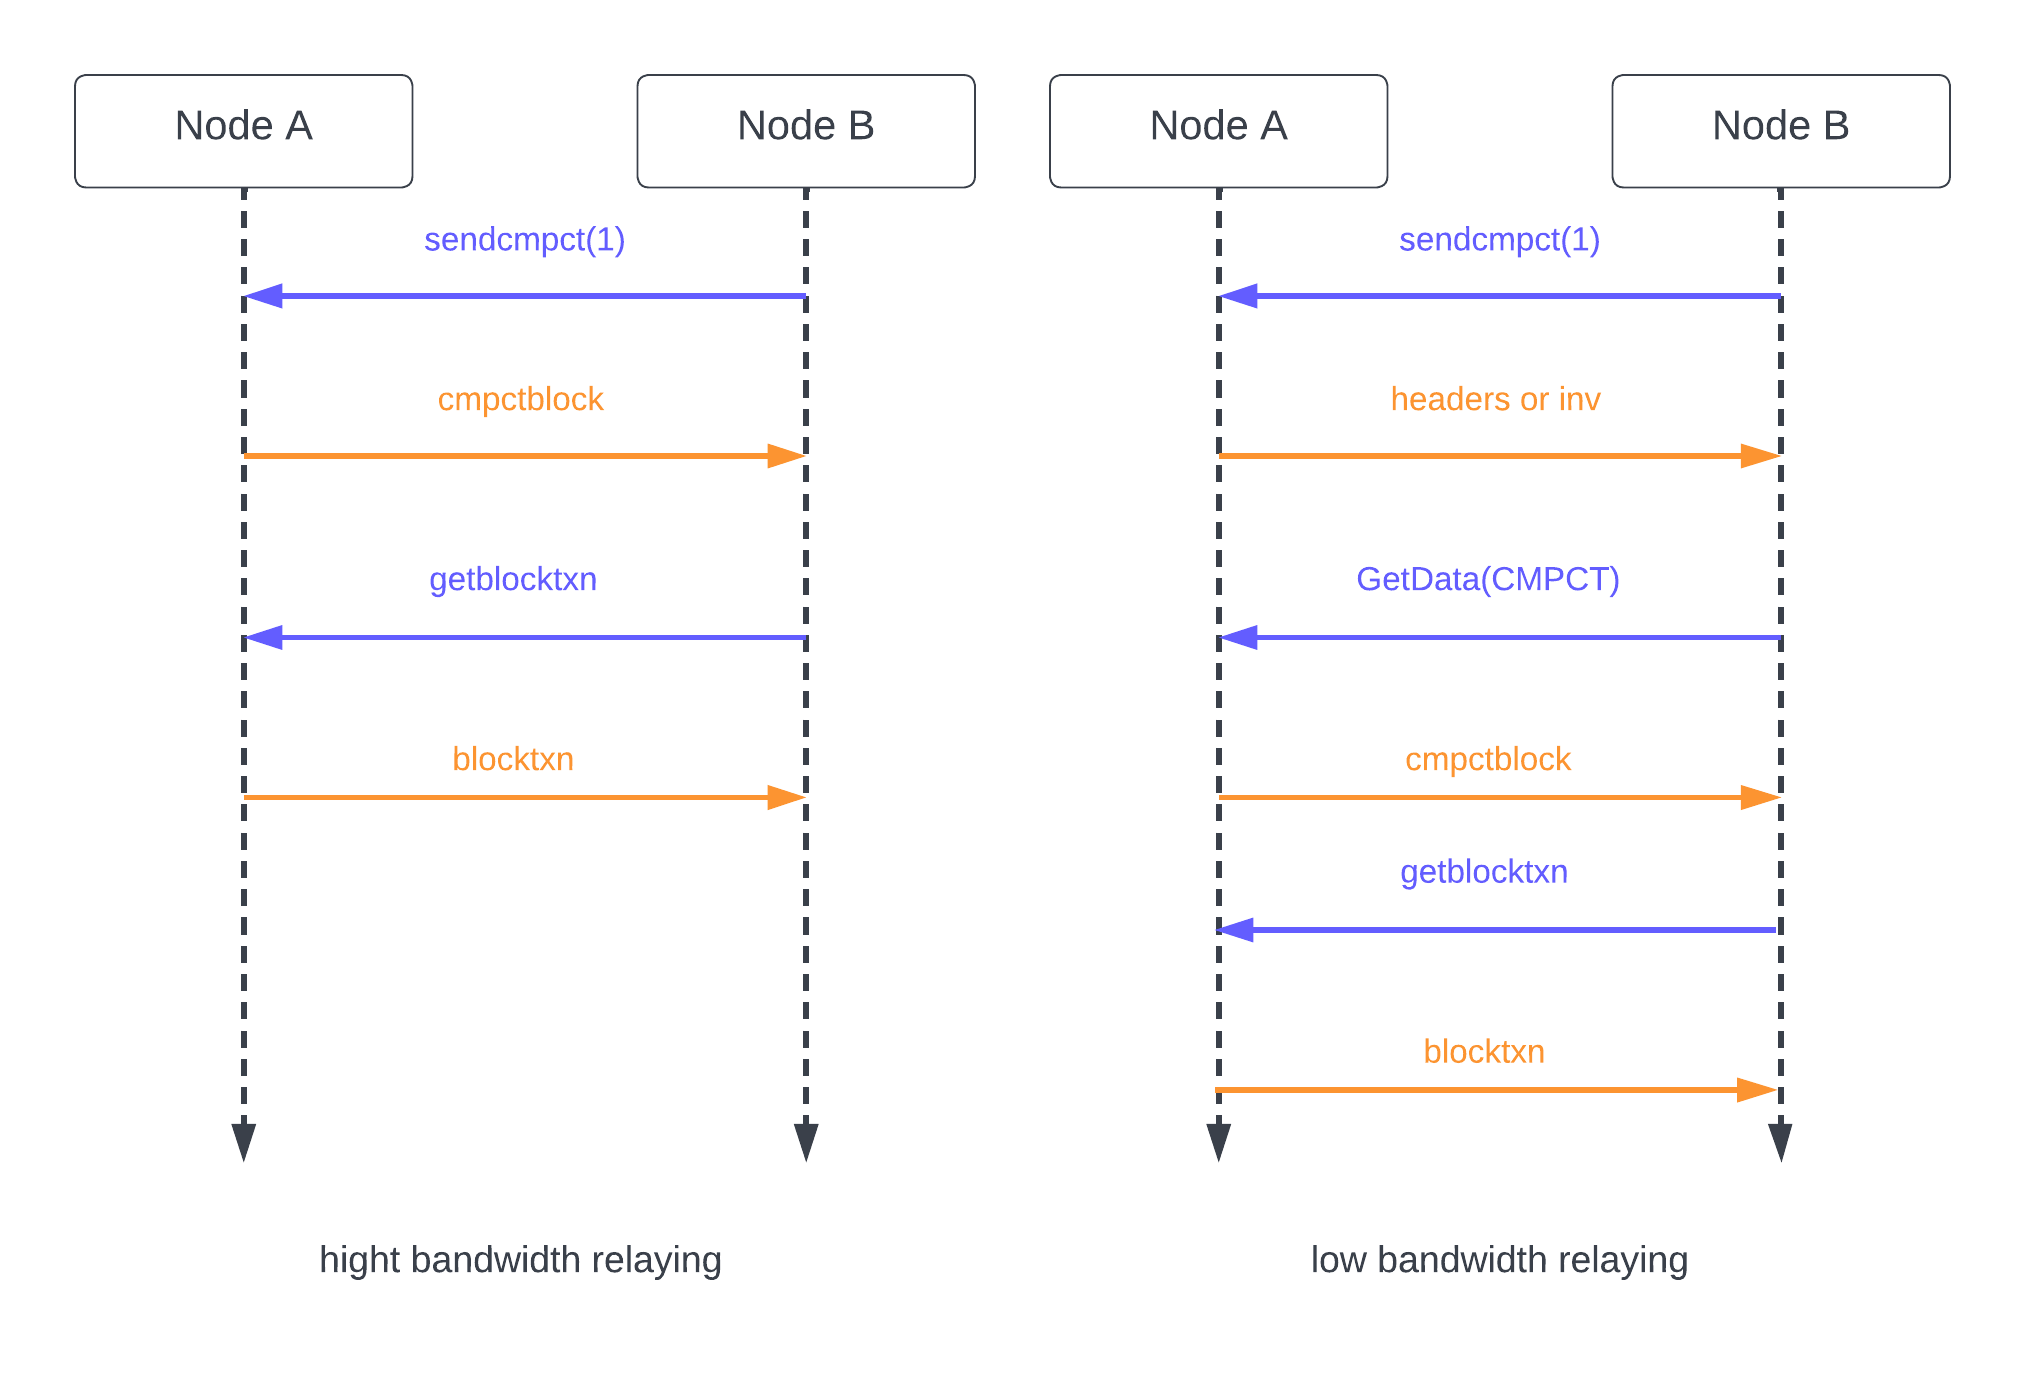
\includegraphics[width=0.8\linewidth]{./Resources/block-compression.png}
			      \caption{Block Compression}
			      \label{fig:block-compression}
		      \end{figure}
		      \item\textbf{Storage scheme Optimization:} This scheme has a consensus unit. It has a number of nodes in it. The blocks of the whole chain are assigned to a single unit. This reduces the total query cost. Jidar is another approach. The main idea is to store only relevant data they are interested in. Small part of the data is stored including the relevant transactions and the merkel branch. If at all we need all the block data, the nodes ask the other nodes and the complete blocks are constructed out of it. There needs to be some incentives for other blocks to help the block asking for the complete data.
	      \end{itemize}
	\item
	      \textbf{Paper Name:} An Empirical Analysis Of Using Blockchain Technology In E-Voting Systems \cite{cadiz2021empirical}\\
	      \textbf{Authors:} J. V. Cadiz, N. A. M. Mariscal and A. M. Ceniza-Canillo\\
	      \textbf{Abstract:} An analysis on the use of blockchain technology in e-voting systems has been done to compare its performance and security to that of a centralized e-voting system. Blockchain technology is one of the emerging technologies of today as a distributed, decentralized database technology, providing much promise to transparency and reducing cybersecurity risks. A Blockchain-based E-Voting System (BEVS) and a Centralized E-Voting System (CEVS) were developed, and compared in terms of performance and security testing. The results show that the BEVS processes requests slightly slower than the CEVS. This is due to the additional processes of block validation and creation in a blockchain network, whereas utilizing a local private blockchain as the database of an e-voting system handles requests faster than utilizing a public blockchain network. However, the BEVS is more reliable when it comes to the efficiency of an e-voting system as it has a complete 0.00\% error rate compared to the CEVS with its errors generated by the internal server. The speed at which the BEVS may also be affected by heavy loads, however, all requests were fulfilled, and no system crashes occurred. The BEVS also proves to be a more secure e-voting system with less vulnerabilities detected.\\
	      \textbf{Inference:}
	      \\This paper discusses the difference between a centralised e-voting system and a blockchain based e-voting system in terms of performance and security. Both systems were designed to have similar interfaces. The only difference between them was the systems used to design the backend. With blockchain based systems, the users needed to use their digital wallet's private key as their credentials to connect to the network. If all the conditions of the contact are satisfied, a new block is created, processed and then added to the blockchain, which serves as the database for this system. The centralised system required users to log in with their voter ID. The votes are processed by the server and stored in a database, which automatically counts the number of votes for each candidate.  Results showed that BEVS is slightly slower than CEVS. This is due to the additional processes of block validation and creation while using a local private blockchain, it processes requests faster than a public blockchain network.  However, the BEVS is more reliable when it comes to efficiency as it has a zero error rate compared to the CEVS with its errors. through the internal server. However, the rate at which the BEVS works can be affected even by heavy loads. The BEVS is also proving to be a more secure electronic voting system with fewer identified vulnerabilities.
	\item
	      \textbf{Paper Name:} A Framework to Make Voting System Transparent Using Blockchain Technology \cite{farooq2022framework}\\
	      \textbf{Authors:} M. S. Farooq, U. Iftikhar and A. Khelifi\\
	      \textbf{Abstract:} A widespread mistrust towards the traditional voting system has made democratic voting in any country very critical. People have seen their fundamental rights being violated. Other digital voting systems have been challenged due to a lack of transparency. Most voting systems are not transparent enough; this makes it very difficult for the government to gain voters’ trust. The reason behind the failure of the traditional and current digital voting system is that it can be easily exploited. The primary objective is to resolve problems of the traditional and digital voting system, which include any kind of mishap or injustice during the process of voting. Blockchain technology can be used in the voting system to have a fair election and reduce injustice. The physical voting systems have many flaws in it as well as the digital voting systems are not perfect enough to be implemented on large scale. This appraises the need for a solution to secure the democratic rights of the people. This article presents a platform based on modern technology blockchain that provides maximum transparency and reliability of the system to build a trustful relationship between voters and election authorities. The proposed platform provides a framework that can be implemented to conduct voting activity digitally through blockchain without involving any physical polling stations. Our proposed framework supports a scalable blockchain, by using flexible consensus algorithms. The Chain Security Algorithm applied in the voting system makes the voting transaction more secure. Smart contracts provide a secure connection between the user and the network while executing a transaction in the chain. The security of the blockchain based voting system has also been discussed. Additionally, encryption of transactions using cryptographic hash and prevention of attack 51\% on the blockchain has also been elaborated. Furthermore, the methodology for carrying out blockchain transactions during the process of voting has been elaborated using Blockchain Finally, the performance evaluation of the proposed system shows that the system can be implemented in a large-scale population.\\
	      \textbf{Inference:}
	      \\This paper explains about the transparent voting system using blockchain technology. It reduces a lot of resources and efforts in the polling system. Unlike the traditional voting system which stores votes on a centralised system, blockchain based voting systems are not easily tampered. Blockchain provides a high level of security that can be trusted more than the previously used technologies.
	      \\Here voters need to complete verification into the voting management system. The nation's database is integrated with the system's database to keep voters’ integrity. For every vote, a transaction is generated against the voter’s National ID then the transaction is saved in blockchain. After casting a vote his/her vote coin is used. After casting vote blockchain verifies his voting system by comparing with the national voting ids. Then miners analyse them to remove malicious votes before adding them to the chain.
	\newpage
	\item
	      \textbf{Paper Name:} Decentralised E-voting system based on Smart Contract by using Blockchain Technology \cite{al2020decentralized}\\
	      \textbf{Authors:} M. Al-madani, A. T. Gaikwad, V. Mahale and Z. A. T. Ahmed\\
	      \textbf{Abstract:} Nowadays the use of the Internet is growing; E-voting system has been used by different countries because it reduces the cost and the time which used to consumed by using traditional voting. When the voter wants to access the E-voting system through the web application, there are requirements such as a web browser and a server. The voter uses the web browser to reach to a centralized database. The use of a centralized database for the voting system has some security issues such as Data modification through the third party in the network due to the use of the central database system as well as the result of the voting is not shown in real-time. However, this paper aims to provide an E-voting system with high security by using blockchain. Blockchain provides a decentralized model that makes the network Reliable, safe, flexible, and able to support real-time services.\\
	      \textbf{Inference:}
	      \\This Paper Explains the Difference between Ballot paper voting and Blockchain based decentralised casting For better integrity of the voting system.
	      \\Here in Decentralised Blockchain System data like the name of voter or votes is saved on a decentralised ledger. This data neither be accessed nor be changed by any third party authority. Currency ballot paper is a widely used voting system worldwide. But this does not guarantee the correctness of the result Due to availability of data at a single resource. This problem is faced by a centralised voting system and is solved by Blockchain based voting systems. Here in Blockchain Technology the data is not stored on a central location but is allotted in different locations on different servers. The data which is distributed across each device connected to the blockchain using a peer-to-peer system.
	      \\In the Decentralised E-voting system candidate registration is done before the voting process starts and then voters identity is verified before the creating account.In this system. The authorised person authenticates the voter and then blockchain ensures the double voting is not allowed.
	\item
	      \textbf{Paper Name:} BlockVOTE : An Architecture of a Blockchain-based Electronic Voting System \cite{angsuchotmetee2019blockvote}\\
	      \textbf{Authors:} C. Angsuchotmetee, P. Setthawong and S. Udomviriyalanon\\
	      \textbf{Abstract:} Electronic voting systems provide many advantages over traditional ballot based voting systems mainly over the accuracy and speed of the tallying process of the voting. However, electronic voting systems suffer from many technical and security issues which have limited its deployment in voting scenarios such as company voting and political elections. Centralized electronic voting systems are, by nature not secure, and there are many avenues of cyber-attacks that could tamper the voting result. Electronic voting system should be highly secured, tamperedproof guaranteed, and the voting should be trusted worthy. In this study, we propose BlockVOTE, a Blockchain-based electronic voting system. Our proposal uses Blockchain to ensure that the voting process can be kept secure and trustable through the consensus handling mechanism of the Blockchain. The architecture design and implementation suggestion are provided in this study. The implementation of the proposal was developed and tested via experimentation. The experiment result and the discussion on the possibility of adopting our proposal in an actual election is provided at the end of this study.\\
	      \textbf{Inference:}
	      \\The paper proposes a Blockchain-based voting system called BlockVOTE. It focuses on keeping the voting system secure and trustable using consensus handling mechanisms. The paper covers Traditional Ballot based Voting systems and Electronic based Voting Systems with both their issues. In the proposed architecture, the paper defines upon processes Poll Creation, Voting and Result Tallying. Authors of the paper implemented the system using Ethereum and HyperLedger and compared the results. The system will have the following actors: Poll Creator, Contract Handler and Voter performing tasks of Poll Creation, Contract creation and deployment and Voting.
	      \begin{figure}[H]
		      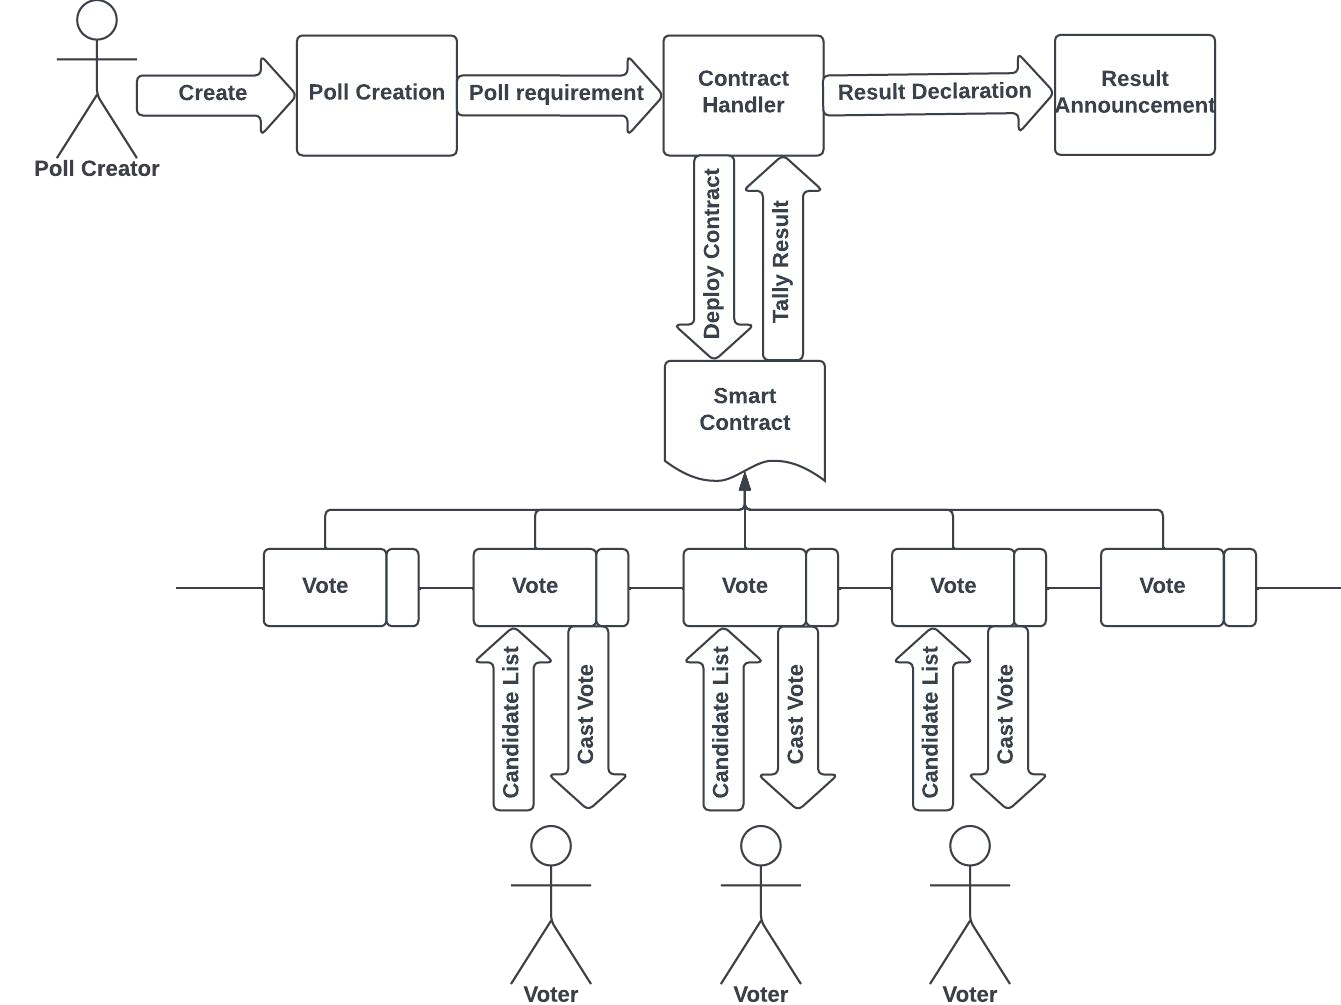
\includegraphics[width=\linewidth]{./Resources/architecture.png}
		      \caption{Blockchain based e-Voting Architecture}
		      \label{fig:evoting-architecture}
	      \end{figure}
	\item
	      \textbf{Paper Name:} Analysis of Blockchain Solutions for E-Voting: A Systematic Literature Review \cite{benabdallah2022analysis}\\
	      \textbf{Authors:} A. Benabdallah, A. Audras, L. Coudert, N. El Madhoun and M. Badra\\
	      \textbf{Abstract:} To this day, abstention rates continue to rise, largely due to the need to travel to vote. This is why remote e-voting will increase the turnout by allowing everyone to vote without the need to travel. It will also minimize the risks and obtain results in a faster way compared to a traditional vote with paper ballots. In fact, given the high stakes of an election, a remote e-voting solution must meet the highest standards of security, reliability, and transparency to gain the trust of citizens. In literature, several remote e-voting solutions based on blockchain technology have been proposed. Indeed, the blockchain technology is proposed today as a new technical infrastructure for several types of IT applications because it allows to remove the TTP and decentralize transactions while offering a transparent and fully protected data storage. In addition, it allows to implement in its environment the smart-contracts technology which is used to automate and execute agreements between users. In this paper, we are interested in reviewing the most revealing e-voting solutions based on blockchain technology.\\
	      \newpage
	      \textbf{Inference:}
	      \\This paper reviews the latest innovations in the  blockchain based e-voting system to understand their particulars and compares them with each other as well as the traditional voting process. Various blockchain based e-voting applications here are being compared based on many parameters like  implementations used, algorithms used, voter identification methods, vote encryption methods, how they fare against attacks and their security properties. After comparing these based on the said factors, limitations and constraints of these systems. Even though the blockchain based systems for voting may be in their initial phases, they offer an interesting solution to the problems of traditional voting.
	\item
	      \textbf{Paper Name:} Blockchain Based E-Voting System: Open Issues and Challenges \cite{khudoykulov2021blockchain}\\
	      \textbf{Authors:} Z. Khudoykulov, U. Tojiakbarova, S. Bozorov and D. Ourbonalieva\\
	      \textbf{Abstract:} Blockchain technology has become very trendy and penetrated different domains, mostly due to the popularity of cryptocurrencies. Blockchain technology offers decentralized nodes for e-voting and is used to create e-voting systems, mainly because of their end-to-end verification benefits. This technology is an excellent replacement for traditional e-voting solutions with distributed performance, reliability and security. The following article provides an overview of e-voting systems based on blockchain technology. The main purpose of this analysis was to examine the current state of blockchain-based voting systems, as well as any associated difficulties in predicting future events.\\
	      \textbf{Inference:}
	      \\This paper analyses current research on blockchain electronic voting systems and identifies issues in it. E-Voting defines the process that uses electronic tools in the process of elections for voting and counting purposes. The procedure for electronic voting varies from country to country. which may include voting machines on polling stations, centralised accounting of paper bills and voting on the Internet. In many countries, centralised calculations are used. Sometimes, however, they also use electronic voting machines in places of voting. However, the use of the internet is minimal. In particular, electronic approaches have been tested in several places and problems with security and reliability were noted. This paper also talks about several factors that makes an e-voting system secure like,
	      \begin{enumerate}[i]
		      \item\textbf{Anonymity:} Any correlation between registered voters and voter identities shall be anonymous.
		      \item\textbf{Auditability and Accuracy:} The results should be accurate and should precisely correspond to the voter sentiment.
		      \item\textbf{Democracy/Singularity:} Every eligible person should be able to vote. There shall be no duplication of votes.
		      \item\textbf{Vote Privacy:} No one should be able to associate a particular vote to an individual.
		      \item\textbf{Robustness and Integrity:} It is the proof that registered voters will abstain without problems. It also encourages others to cast their legitimate votes.
		      \item\textbf{Transparency and Fairness:} No one outside the people involved with the counting process can find out about the results before they are announced.
		      \item\textbf{Availability and Mobility:} The systems should always be available during the electoral process.
		      \item\textbf{Verifiable Participation/Authenticity:} The authorities should be able to check if someone abstained from voting.
		      \item\textbf{Recoverability and Identification:} It should be able to track and restore data in order to avoid attacks or data losses.
	      \end{enumerate}
	      \begin{figure}[H]
		      \centering
		      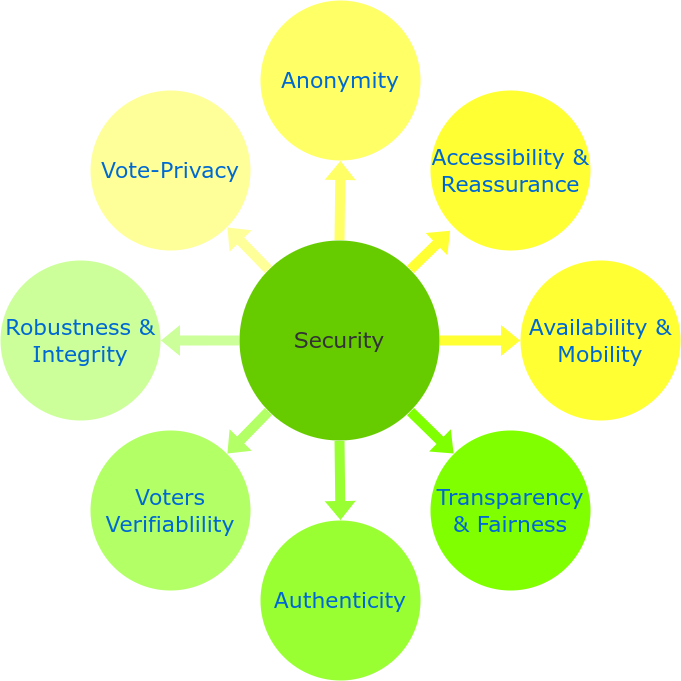
\includegraphics[width=0.6\linewidth]{./Resources/security-requirements.png}
		      \caption{Security Requirements for Electronic Voting System}
		      \label{fig:security-requirements}
	      \end{figure}
	\item
	      \textbf{Paper Name:} Blockchain for Electronic Voting System—Review and Open Research Challenges \cite{jafar2021blockchain}\\
	      \textbf{Authors:} Jafar, Uzma, Mohd Juzaiddin Ab Aziz, and Zarina Shukur\\
	      \textbf{Abstract:} Online voting is a trend that is gaining momentum in modern society. It has great potential to decrease organizational costs and increase voter turnout. It eliminates the need to print ballot papers or open polling stations—voters can vote from wherever there is an Internet connection. Despite these benefits, online voting solutions are viewed with a great deal of caution because they introduce new threats. A single vulnerability can lead to large-scale manipulations of votes. Electronic voting systems must be legitimate, accurate, safe, and convenient when used for elections. Nonetheless, adoption may be limited by potential problems associated with electronic voting systems. Blockchain technology came into the ground to overcome these issues and offers decentralized nodes for electronic voting and is used to produce electronic voting systems mainly because of their end-to-end verification advantages. This technology is a beautiful replacement for traditional electronic voting solutions with distributed, non-repudiation, and security protection characteristics. The following article gives an overview of electronic voting systems based on blockchain technology. The main goal of this analysis was to examine the current status of blockchain-based voting research and online voting systems and any related difficulties to predict future developments. This study provides a conceptual description of the intended blockchain-based electronic voting application and an introduction to the fundamental structure and characteristics of the blockchain in connection to electronic voting. As a consequence of this study, it was discovered that blockchain systems may help solve some of the issues that now plague election systems. On the other hand, the most often mentioned issues in blockchain applications are privacy protection and transaction speed. For a sustainable blockchain-based electronic voting system, the security of remote participation must be viable, and for scalability, transaction speed must be addressed. Due to these concerns, it was determined that the existing frameworks need to be improved to be utilized in voting systems.\\
	      \textbf{Inference:}
	      \\A blockchain includes the following components:
	      \begin{enumerate}[i]
		      \item\textbf{Node:} It refers computer or user participating in the blockchain network.
		      \item\textbf{Transaction:} The is the data stored in blocks making it the most fundamental part of a blockchain system.
		      \item\textbf{Block:} It is the data structure which is used for storing the transaction information.
		      \item\textbf{Chain:} A sequence of blocks which are organized in some specific order.
		      \item\textbf{Miners:} Specific nodes which perform the block verification process.
		      \item\textbf{Consensus:} Algorithm which ensures validity of block and decides whether it should be inserted to chain or not.
	      \end{enumerate}
	      \begin{figure}[H]
		      \centering
		      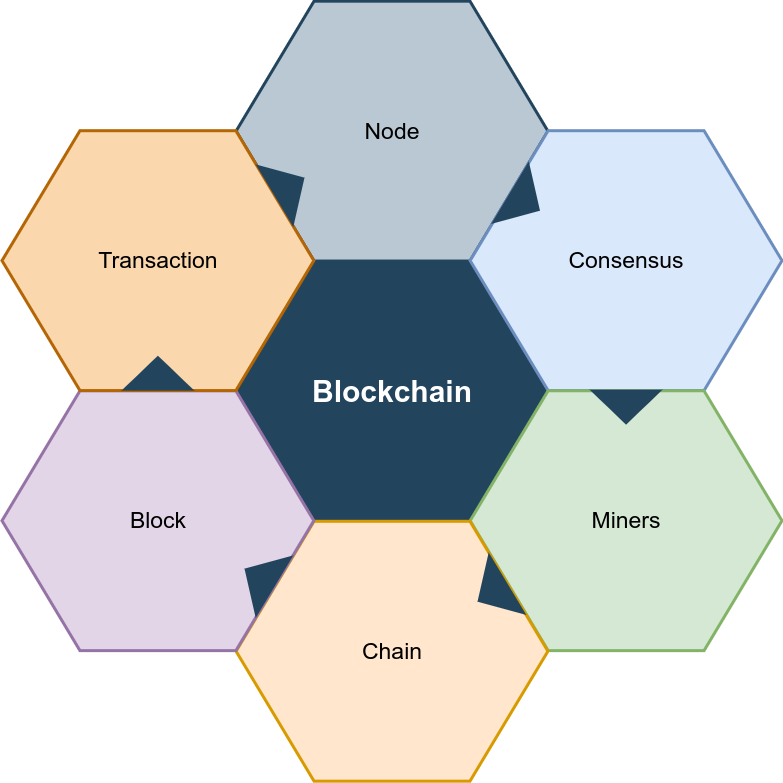
\includegraphics[width=0.6\linewidth]{./Resources/core-components.png}
		      \caption{Core Components of Blockchain Architecture}
		      \label{fig:core-components}
	      \end{figure}
\end{enumerate}
\subsection{Outcome of Literature Survey}
Blockchain is a new emerging technology. It is currently under research to implement with perfection. Blockchain has shown some promising applications. Some of its famous applications include finance industry, healthcare industry, art industry etc. The concept of blockchain was proposed in 2008 by a person named Satoshi Nakamoto and was actualized a year later. Based on the application of the blockchain there are different characteristics of it that make it different. They are cost effective. Reduces the overall cost of conducting transactions on our case voting. There is no need for a central agency. Persistence helps us keep track of all the logs of voting in the system. There are three roles in the blocks. The one who proposes a transaction/vote. The one who checks or validates whether the votes are valid or not and applies it to itself. And lastly the one who learns from all these transactions and implements the votes to itself. Blockchain systems provides you with anonymity over traditional systems. They do not collect the users private data. The blocks added to the system remain there forever. This facilitates auditing of the transaction or in our cases votes. There are different tradeoffs to make blockchain scalable. Lately there was a fork made to bitcoin to increase its scalability. Bitcoin having a block size of 1MB could accommodate a smaller number of transactions, whereas the fork (now known as bitcoin-cash) has a block size of 8-32 MB. This increases the number of transactions that can be accommodated in a block. Another technique to increase scalability is to tweak the data structure of the block. It calculates the transaction IDs in the memory pool and matches it with the transaction IDs in the compact block.
\\\textbf{Advantages:}
\begin{enumerate}
	\item The votes cannot be manipulated as consensus algorithms are used.
	\item Before a node (i.e a vote) is added to the chain, its legitimacy is verified by various nodes in the network.
	\item Every node in the network has a copy of the ledger and therefore the transparency of the process increases.
	\item There is no central server/system which reduces the possibility of data loss and malicious attacks.
	\item Also since there is no central server/system it increases the reliability of the system as there is no single point of failure.
	\item The counting process also becomes more efficient and use of blockchain increases the accuracy of the system.
	\item Mechanisms can be put in place to prevent duplicate voting.
\end{enumerate}
\textbf{Disadvantages:}
\begin{enumerate}
	\item As the number of nodes increases, the amount of time required to process a transaction also increases.
	\item There is a chance that the voters can be intimidated or coerced to vote against their will.
	\item There needs to be proper power supply and backup in order for the system to function seamlessly.
	\item As blockchain is resource intensive the cost of hardware increases and power consumption increases.
	\item If the number of active nodes decrease then the security of the blockchain aso decreases.
	\item People in general are reluctant to use new technology.
	\item As the number of nodes increases, it becomes increasingly difficult to maintain the nodes.
\end{enumerate}
\subsection{Conclusion of Literature Survey}
As we have seen, all the above-mentioned papers have their own advantages. By evaluating all the advantages we can develop the platform for blockchain based E-voting systems. The proposed platform provides a framework that can be implemented to conduct voting activity digitally through blockchain without involving any malpractices. Our goal is to create an E-voting system that can be trusted by voters and to encourage them to vote.
\newpage
\section{Problem Statement and Scope}
\newpage
\subsection{Problem Statement}
Blockchain technology can be used in the E-voting system to conduct a fair election and reduce injustice. The physical voting systems have many flaws in it as well as the digital voting systems are not perfect enough to be implemented on a large scale. Our aim here is to create a private network responsible for storing and maintaining blockchain. Upon this network, develop a decentralized blockchain based Voting System system based on smart contract which is the optimum solution for frauds, forgery, human error, traceability, stagnancy occurring in the current system providing enhanced security, privacy, efficiency and speed in the Voting  process.
\subsubsection{Goals and Objectives}
To design a decentralized e-voting system that,
\begin{enumerate}
	\item Reduces human interaction in the process of voting and elections in general.
	\item Does not depend on a trusted third party for controlling the collected data, whilst still staying immune to attacks and guaranteeing user privacy.
	\item Provides transparency, ensuring security and does not jeopardize voter privacy.
\end{enumerate}
\subsubsection{Scope}
Blockchain technology has proven itself in recent years as a tamper proof solution to store information. When it comes to lack of trust in the system and possibility of cheating we can trust on blockchain. Blockchain is almost unhackable with traditional techniques providing exceptional security. The goal of this project is to reduce corruption and conduct fair elections. The scope currently is to provide the proof of concept and then scale it. Also in order to scale it we need to do the potential tradeoffs to optimize performance and reduce the harm it causes to the environment. Using efficient algorithms to reduce the number of calculations required.
\subsection{Major Constraints}
\begin{enumerate}
	\item The application should be able to manage a high amount of requests and transactions while maintaining the correctness of the results.
	\item The application must also ensure that the identities and personal information of the users are safeguarded.
	\item The systems must be usable by all users, regardless of their technological abilities or accessibility requirements.
\end{enumerate}
\subsection{Expected Outcome}
\begin{enumerate}
	\item Promote transparency in the electoral process.
	\item Improve security by encrypting vote data and preventing unauthorized access.
	\item All transactions are recorded on a public ledger that cannot be altered, which can also help to prevent tampering with voting results.
	\item The automation of numerous electoral processes, such as vote counting and auditing.
\end{enumerate}
\subsection{Applications}
\begin{enumerate}
	\item A decentralized voting application can be used for corporate governance, allowing shareholders to vote on crucial issues such as mergers, acquisitions, and board appointments.
	\item A decentralized voting application can be used for public opinion polls, allowing people to voice their views on political, social, and economic topics in a secure and anonymous manner.
	\item A decentralized voting application can be used in community governance, allowing members of a community to vote on crucial choices such as community initiatives, resource allocation, and public works.
	\item Referendums can be held using a decentralized voting application, which allows citizens to vote on key matters such as constitutional amendments, changes in public policy, and large infrastructure projects.
\end{enumerate}
\newpage
\section{Project Plan}
\newpage
\subsection{Project Estimates}
Use Agile model and associated streams derived from assignments 1,2,3,4 and5 (Annex A and B) for estimation.
\subsubsection{Sequential Phases in Agile Methodology}
The software development model that is used in this project is Agile Model. It is an iterative and incremental approach to software development that emphasizes collaboration, flexibility and adaptability. It consists of the following stages:
\begin{figure}[H]
	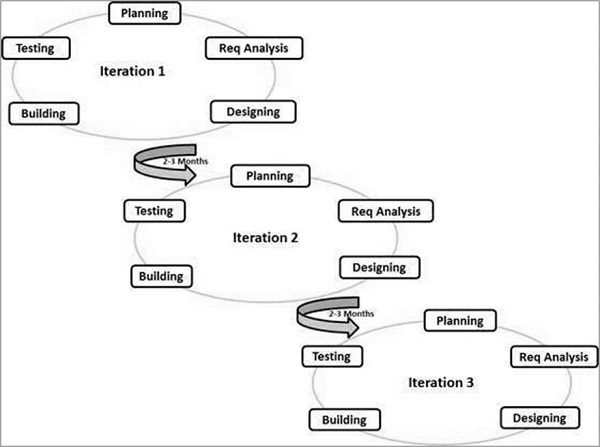
\includegraphics[width=\linewidth]{./Resources/agile.png}
	\caption{Agile Methodology}
	\label{fig:agile}
\end{figure}
\begin{enumerate}
	\item \textbf{Planning :} During this stage, the development team determines the project's needs and scope. Following that, the team develops a plan outlining the tasks and deliverables for each sprint.
	\item \textbf{Requirements analysis :} In this stage, the development team improves the requirements and builds user stories. User stories are brief descriptions of features written from the perspective of the end user.
	\item \textbf{Design :} Based on the requirements and user stories, the development team designs a design for the feature or product at this stage.
	\newpage
	\item \textbf{Implementation :} The development team constructs the feature or product according to the design at this stage. This stage is frequently divided into smaller sprints, with each sprint producing a functional product or feature.
	\item \textbf{Testing :} The development team tests the feature or product at this stage to confirm that it meets the requirements and is free of faults and defects.
	\item \textbf{Deployment :} The feature or product is deployed to the client or end-users at this step. During this stage, the development team may also provide training and support to the customer.
	\item \textbf{Review :} At this point, the development team and the customer go over the sprint outcomes and provide input. This feedback is utilized to improve the design and implementation of the feature or product by refining the requirements.
\end{enumerate}
\subsubsection{Project Resources}
Well configured Laptop, 8 GB RAM, 40 GB Storage, Intel i5 Processor, Remix IDE.
\subsection{Risk Management}
The process of identifying the risk (Product risk or Project risk) , analyzing the risk, and then mitigating the risk or controlling the risk is known as Risk Management. We identified following risks that were managed as below:
\subsubsection{Risk Identification}
Risk management begins with risk identification. By utilizing certain approaches, we must identify both project and product risk. The use of risk-free templates, stakeholder interviews, project retrospectives, etc. are some of the most popular methods that may be used to detect various risks.
\begin{itemize}
	\item Risk: Risk is the expectation of suffering a loss or encountering a potential issue in the future, whether or not it does so. Usually, it results from a lack of knowledge, power, or time. A software risk is the potential for financial loss during the software development process.
	\item Product Risk: Risks associated with a software product or programme that may develop as a result of its inability to function as users want it to. These risks include any kind of unforeseen or unpredictable incident or activity that could happen and harm a project's progress.
	\item Some of the classic strategies include:
	      \begin{enumerate}
		      \item Avoid it: Sometimes a plan can be developed to entirely prevent a risk. It might be conceivable to use a different supplier, for instance, if there is a chance that a certain one will supply a necessary item too late to meet your deadline.
		      \item Accept it: It might not be worthwhile to handle the risk at all if the impact and probability are low.
		      \item Reduce it: Establishing contingency plans and funding, adding team members with the knowledge to take over a crucial task in the event that others leave, and cultivating a favorable relationship with persons outside the team whose cooperation is crucial for success are some approaches to decrease risks.
		      \item Transfer it: In some cases, you can delegate control of a particular risk to a supplier, an independent consultant, or even a stakeholder.
	      \end{enumerate}
\end{itemize}
\subsubsection{Risk Analysis}
\begin{table}[H]
	\centering
	\begin{tabular}{|l|l|l|}
		\hline
		\multicolumn{1}{|c|}{Probability} & \multicolumn{1}{c|}{Value}   & \multicolumn{1}{c|}{Description} \\ \hline
		High                              & Probability of occurrence is & \textgreater 75\%                \\ \hline
		Medium                            & Probability of occurrence is & 26 – 75 \%                       \\ \hline
		Low                               & Probability of occurrence is & \textless 25\%                   \\ \hline
	\end{tabular}
	\caption{Risk Probabilities}
	\label{tab:risk-probabilities}
\end{table}
\begin{table}[H]
	\centering
	\begin{tabular}{|l|l|l|}
		\hline
		Impact    & Value              & Description                                                                                                                                                   \\ \hline
		Very High & \textgreater 10 \% & Schedule impact or Unacceptable quality                                                                                                                       \\ \hline
		High      & 5 – 10 \%          & \begin{tabular}[c]{@{}l@{}}Schedule impact or some parts of the project have low\\ quality\end{tabular}                                                       \\ \hline
		Medium    & \textless 5 \%     & \begin{tabular}[c]{@{}l@{}}Schedule impact or barely noticeable degradation in\\ quality Low impact on schedule or Quality can be\\ incorporated\end{tabular} \\ \hline
	\end{tabular}
	\caption{Risk Impact Definitions}
	\label{tab:risk-impact-definitions}
\end{table}
%\subsubsection{Overview of Risk Mitigation, Monitoring, Management}
%Following are the details for each risk.
\subsection{Project Schedule}
\subsubsection{Project Task Set}
Major Tasks in the Project stages are:
\begin{itemize}
	\item Task 1: Correctness
	\item Task 2: Availability
	\item Task 3: Integrity
\end{itemize}
\subsubsection{Task Network}
Project tasks and their dependencies are noted in this diagrammatic form.
\begin{figure}[H]
	\centering
	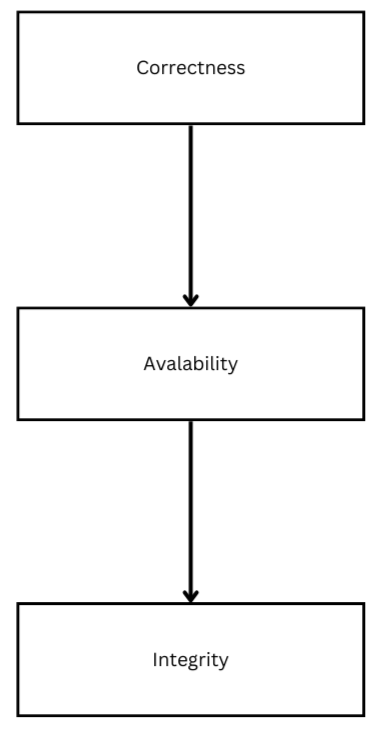
\includegraphics[width=0.4\linewidth]{./Resources/task-network.png}
	\caption{Task Network}
	\label{fig:task-network}
\end{figure}
\subsubsection{Timeline Chart}
A project timeline chart is presented. This may include a timeline for the entire project. Above points is also covered in Project Planner as Annexure B.
\subsection{Team Organization}
Team consists of 4 members and proper planning mechanism is used androles of each member are defined.
\subsubsection{Team Structure}
The team structure for the project is identified. There is total 4 members in our team and roles are defined. All members are contributing in all the phases of project.
\begin{table}[H]
	\resizebox{\textwidth}{!}{%
		\begin{tabular}{|l|l|l|l|}
			\hline
			Month Scheduled     & Phase                                                                              & Members             & Work Done                                                                                                     \\ \hline
			July - August       & Topic searching                                                                    & All                 & Topic Searched                                                                                                \\ \hline
			August-September    & Topic selection                                                                    & All                 & Topic Selected and finalized                                                                                  \\ \hline
			August-September    & Project Confirmation                                                               & All                 & \begin{tabular}[c]{@{}l@{}}Project approved by Internal\\ and External guide\end{tabular}                     \\ \hline
			August-September    & Literature Survey                                                                  & All                 & Literature Survey was done                                                                                    \\ \hline
			September – October & Requirement Analysis                                                               & All                 & \begin{tabular}[c]{@{}l@{}}Requirement analysis was\\ done\end{tabular}                                       \\ \hline
			October-November    & \begin{tabular}[c]{@{}l@{}}Survey paper\\ publishing\end{tabular}                  & All                 & Survey Paper Published                                                                                        \\ \hline
			November-December   & Network Creation                                                                   & Yash                & A private network was created                                                                                 \\ \hline
			December-January    & \begin{tabular}[c]{@{}l@{}}Creation of Blockchain\\ and Genesis Block\end{tabular} & Yash, Arvind        & \begin{tabular}[c]{@{}l@{}}Blockchain was implemented\\ and genesis block was created\end{tabular}            \\ \hline
			December-January    & \begin{tabular}[c]{@{}l@{}}Implementation of\\ Solidity Contracts\end{tabular}     & Arvind, Gaurav      & \begin{tabular}[c]{@{}l@{}}Solidity Contracts were\\ implemented for voting and\\ authentication\end{tabular} \\ \hline
			January-February    & \begin{tabular}[c]{@{}l@{}}Implementation of\\ Front End using React\end{tabular}  & Gaurav              &                                                                                                               \\ \hline
			February-March      & \begin{tabular}[c]{@{}l@{}}Optimization and\\ Performance Evaluation\end{tabular}  & Shree, Gaurav       &                                                                                                               \\ \hline
			March-April         & \begin{tabular}[c]{@{}l@{}}Code Integration and\\ testing\end{tabular}             & Shree, Yash, Gaurav & \begin{tabular}[c]{@{}l@{}}Code was combined and test\\ cases were generated\end{tabular}                     \\ \hline
			April-May           & \begin{tabular}[c]{@{}l@{}}Implementation Paper\\ Publishing\end{tabular}          & All                 & \begin{tabular}[c]{@{}l@{}}Implementation Paper\\ Published\end{tabular}                                      \\ \hline
			April-May           & Documentation                                                                      & All                 & Documentation Done                                                                                            \\ \hline
		\end{tabular}%
	}
	\caption{Team Structure Phases}
	\label{tab:team-structure-phases}
\end{table}
\subsubsection{Management reporting and communication}
\begin{itemize}
	\item Well planning mechanisms are used for progress reporting and inter/intra team communication is identified as per requirements of the project.
	\item Each team member had worked on modules. Each unit was worked on and finished simultaneously. After the competition of all modules, unit testing was performed, Final modules were integrated together, and integration testing was performed.
\end{itemize}
\newpage
\section{Software Requirement Specification}
\newpage
\subsection{Introduction}
\subsubsection{Purpose and Scope of Document}
A software requirements specification is the basis for your entire project. It lays the framework that every team involved in development will follow. It is used to provide critical information to multiple team’s development quality assurance, operations, and maintenance. This keeps everyone on the same page. Using the SRS helps to ensure requirements are fulfilled: And it can also help you make decisions about your products lifecycle for instance, when to retire a feature. Writing an SRS can also minimize overall development time and costs. Embedded development teams especially benefit from using an SRS.
\subsubsection{Overview of responsibilites of Developer}
A Developer must perform project design and development activities according to customer specifications. Work with Manager in developing the project plan, budget, and schedule. He has to coordinate with management in preparing project proposals and contractual documents. A Project developer has to keep track of project progress regularly and develop status reports to management. Ensure that the project is completed within the allotted budget and timelines. Follow company policies and safety regulations for operational efficiency, Other responsibilities consist of research and recommend new technologies to carry out project development tasks. Provide assistance to other Developers, perform peer reviews and provide feedback for improvements. To develop cost reduction mitigative while maintaining quality and productivity.
\subsection{System Requirements}
\subsubsection{System Interface}
\textbf{Hardware Interface}
\begin{itemize}
	\item\textbf{RAM :} 8 GB (As we are using Blockchain hosted on private networks. Hence  minimum Ram requirement is 8 GB)
	\item\textbf{Hard Disk :} 40 GB
	\item\textbf{Processor :} Intel i5 Processor
\end{itemize}
\textbf{Software Interface}
\begin{itemize}
	\item\textbf{Operating System :} Portable. Latest Operating System that supports all types of installation and development Environment.
	\item\textbf{IDE :} Remix IDE for Solidity Smart Contracts. It is a robust toolbox that users of any skill level can utilize for the whole process of contract development and deployment.
	\item\textbf{Languages :} Solidity, JavaScript, HTML, CSS, Python
\end{itemize}
\subsection{Usage Scenarios}
\subsubsection{User profiles}
\begin{enumerate}
	\item Voter : The voter has limited access to the system. His function is to register. Then to register. There will be a provision to give him a coin. The coin will be consumed when the voter casts a vote.
	\item Admin : The admin is mostly the moderator of the system. He has access to the candidate data. The voter data will be anonymous. But candidate data will be accessible. He can add different parties in the voting system.
	\item Candidate : Candidates basically define a party. They are basically the on which voters vote. Candidates are registered by admins. They can only see the results in their dashboard . They cannot cast votes.
\end{enumerate}
\subsubsection{Use Case View}
\begin{figure}[H]
	\centering
	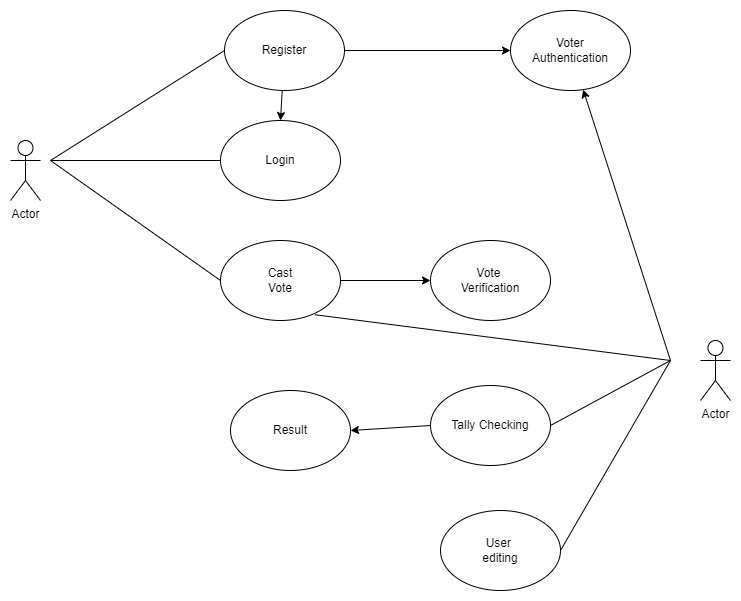
\includegraphics[width=\linewidth]{./Resources/use-case.png}
	\caption{Use Case Diagram}
	\label{fig:use-case}
\end{figure}
\subsection{Data Model and Description}
\subsubsection{Data Description}
Data objects that will be managed/manipulated by the software are described in this section. The database entities or files or data structures required to be described. For data objects details can be given as below.
\subsubsection{Data Objects and Relationships}
Data objects and their major attributes and relationships among data objects are described using an ERD like form.
\subsection{Functional Model and Description}
A description of each major software function, along with data flow (structured analysis) or class hierarchy (Analysis Class diagram with class description for object-oriented system) is presented.
\subsubsection{Data Flow Diagram}
\begin{figure}[H]
	\centering
	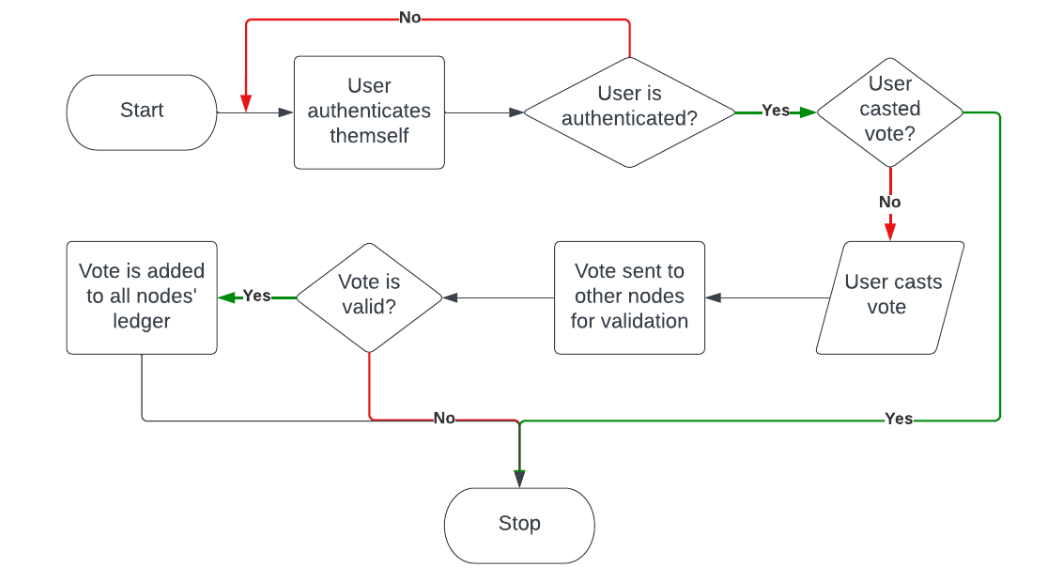
\includegraphics[width=\linewidth]{./Resources/data-flow.png}
	\caption{Data Flow Diagram}
	\label{fig:data-flow}
\end{figure}
\subsubsection{Activity Diagram}
\begin{figure}[H]
	\centering
	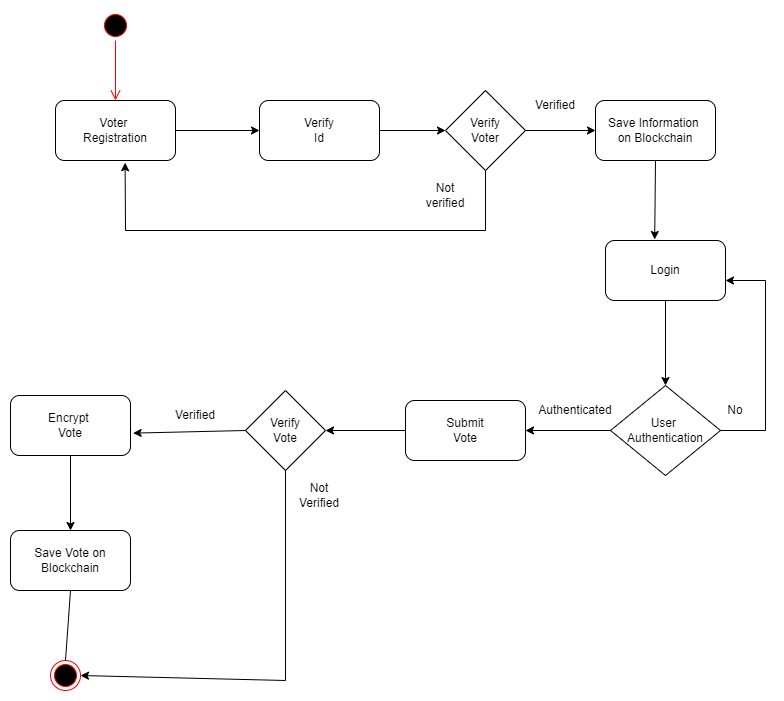
\includegraphics[width=\linewidth]{./Resources/activity.png}
	\caption{Activity Diagram}
	\label{fig:activity}
\end{figure}
\subsubsection{Non-Functional Requirements}
\begin{itemize}
	\item\textbf{Performance Requirements}\\The performance of the functions and every module must be well. The overall performance of the software will enable the users to work efficiently. Performance of encryption of data should be fast.
	\item\textbf{Safety Requirement}\\The application is designed in modules where errors can be detected and fixed easily. This makes it easier to install and update new functionality if required.
	\item\textbf{Software Quality Attributes}\\Our software has many quality attribute that are given below:
	\begin{enumerate}
		\item\textbf{Adaptability :} This software is adaptable by all users.
		\item\textbf{Maintainability :} After the deployment of the project if any error occurs then it can be easily maintained by the software developer.
		\item\textbf{Reliability :} The performance of the software is better which will increase the reliability of the Software.
		\item\textbf{User Friendliness :} Since, the software is a GUI application; the output generated is much user friendly in its behavior.
		\item\textbf{Integrity :} Integrity refers to the extent to which access to software or data by unauthorized persons can be controlled.
		\item\textbf{Security :} Users are authenticated before casting votes.
		\item\textbf{Test ability :} The software will be tested considering all the aspects.
	\end{enumerate}
\end{itemize}
\subsubsection{Design Constraints}
Any design constraints that will impact the subsystem are noted.
\subsubsection{Software Interface Description}
The first screen that appears as the module is started is the Login Page which asks for user credentials to log in to the system.
\\\\After the user is logged in, he will be greeted with another page, where he would have a choice to vote for a candidate from multiple choices.
\\\\For admin there is an Admin Dashboard where he can monitor voters who have votes as well as the number of votes of the candidates.
\newpage
\section{Detailed Design Document using Annexure A and B}
\newpage
\subsection{Introduction}
India is said to have the largest democracy. For the electoral voting system India is using modern “Electronic Voting Machines” which are responsible for taking user input and storing the votes entered by the end user. Later these votes are carried to a central location where they are counted and the result is declared. Though, there is a possibility that these votes data can be tampered with. Having a single central server to store data creates a single point of failure for the entire system. These issues cause mistrust regarding the current system. In the traditional ballot paper system, vote authenticity was questionable and had its separate issues for which it was replaced with modern Electronic Voting Machines.
\\\\Blockchain is based on Distributed Ledger Technology(DLT). In DLT, replicas of the same data are made on different nodes in the network due to which there is no single point of failure. Moreover, due to consensus algorithms implemented in blockchain, all nodes decide and agree upon whether a block is valid and must be added to the network or not
\\\\Decentralized voting systems can provide increased transparency, as they often rely on blockchain technology or other distributed ledger systems. Every vote cast can be recorded on the blockchain, making the process transparent and verifiable by anyone. This transparency helps build trust in the integrity of the voting system.  Centralized voting systems are vulnerable to various security risks, such as hacking, tampering, or manipulation of results. In contrast, decentralized voting systems leverage the security features of blockchain technology, which makes it extremely difficult for any single entity or malicious actor to tamper with the results. Each vote is recorded in a transparent and immutable manner, ensuring the integrity of the voting process.
\\\\In centralized voting systems, there is a risk of censorship by the central authority. Decentralized voting systems aim to mitigate these risks by empowering individual voters to directly participate and control their votes. By removing the need for intermediaries, decentralized systems provide a higher level of autonomy and reduce the potential for manipulation or censorship.
\subsection{Architectural Design}
The architecture of a system describes its major components, their relationships (structures), and how they interact with each other. Software architecture and design includes several contributory factors such as Business strategy, quality attributes, human dynamics, design and IT environment.
\begin{figure}[H]
	\centering
	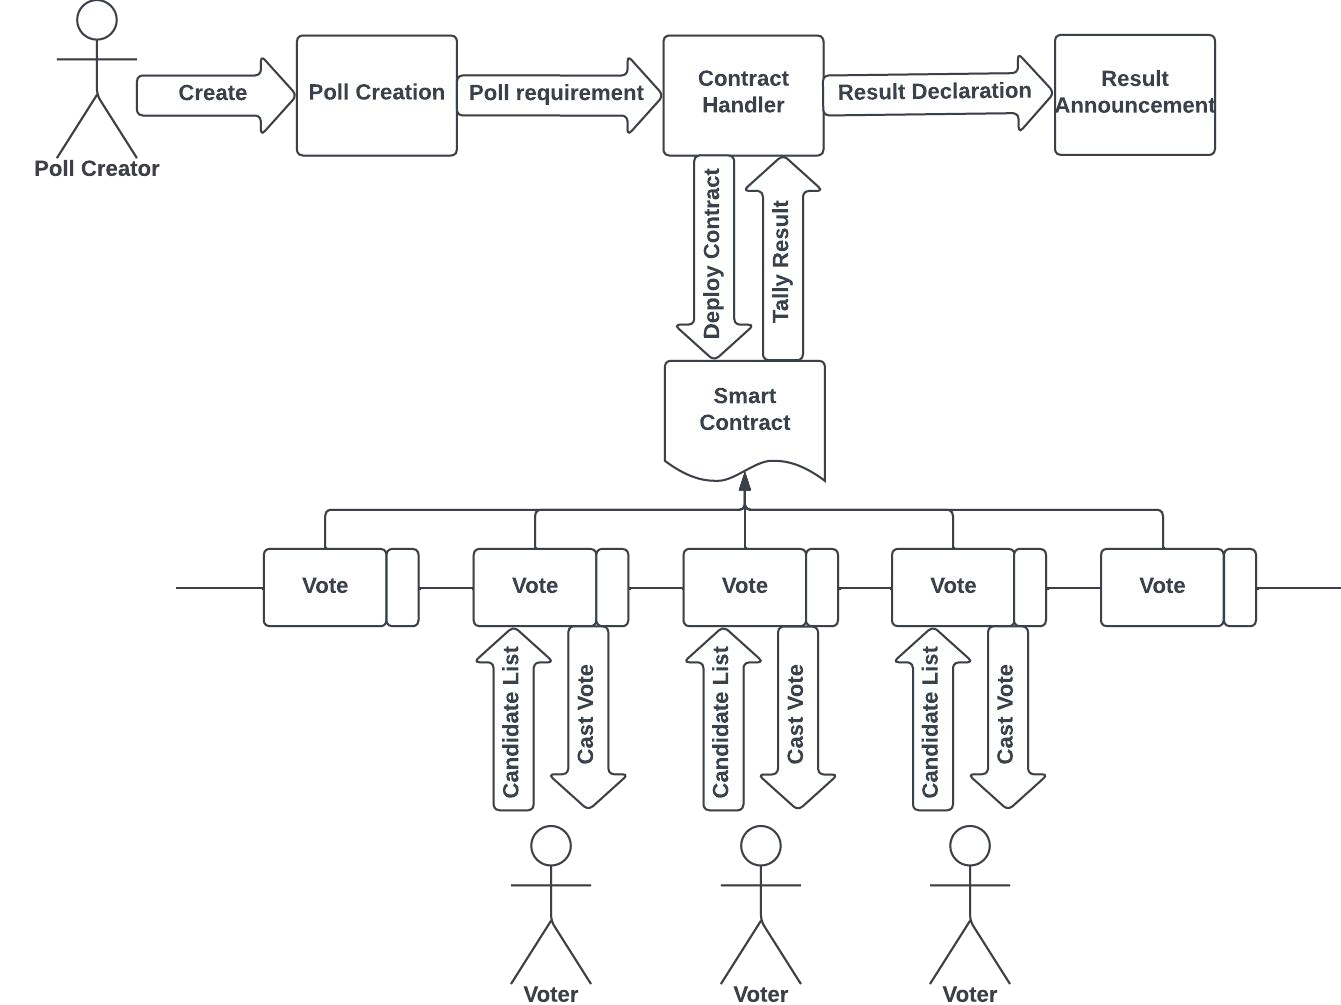
\includegraphics[width=\linewidth]{./Resources/architecture.png}
	\caption{Architecture Diagram}
	\label{fig:architecture}
\end{figure}
\subsection{Data Design (Using Annexure A and B)}
\subsubsection{Internal Software Data Structure}
Data design is the first design activity, which results in less complex, modular and efficient program structure. The information domain model developed during the analysis phase is transformed into data structures needed for implementing the software. The data objects, attributes and relationships depicted in entity relationship diagrams and the information stored in data dictionaries provide a base for data design activity. During the data design process, data types are specified along with the integrity rules required for the data.
\subsubsection{Database Description}
In a Blockchain network LevelDB is used to store the blocks. LevelDB is an open-source key-value storage library developed by Google. It is designed to provide a simple, lightweight, and efficient solution for storing and retrieving data. LevelDB is written in C++ and provides bindings for various programming languages, making it accessible for developers across different platforms.
\subsection{Component Design}
Component diagrams are used in modeling the physical aspects of object-oriented systems that are used for visualizing, specifying, and documenting component- based systems and also for constructing executable systems through forward and reverse engineering. Component diagrams are essentially class diagrams that focus on a system’s components that are often used to model the static implementation view of a system.
\begin{figure}[H]
	\centering
	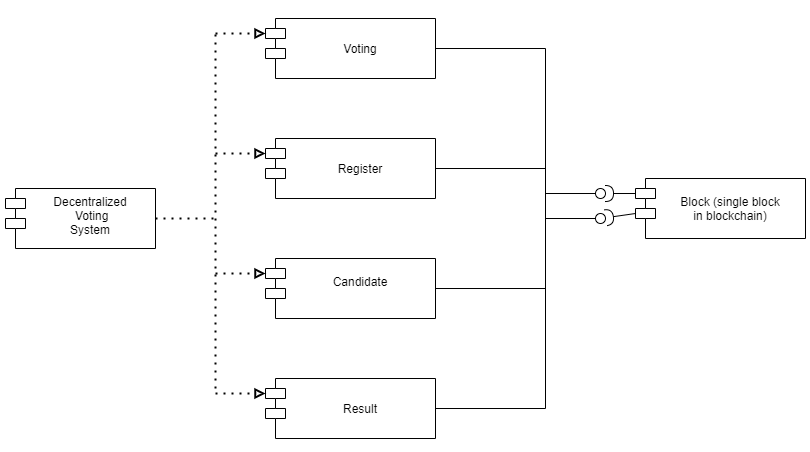
\includegraphics[width=\linewidth]{./Resources/component.png}
	\caption{Component Diagram}
	\label{fig:component}
\end{figure}
\newpage
\subsubsection{Class Diagram}
In software engineering, a class diagram in the Unified Modeling Language (UML) is a type of static structure diagram that describes structure of a system by showing the system’s classes, their attributes, operations (or methods), and the relationships among objects.
\begin{figure}[H]
	\centering
	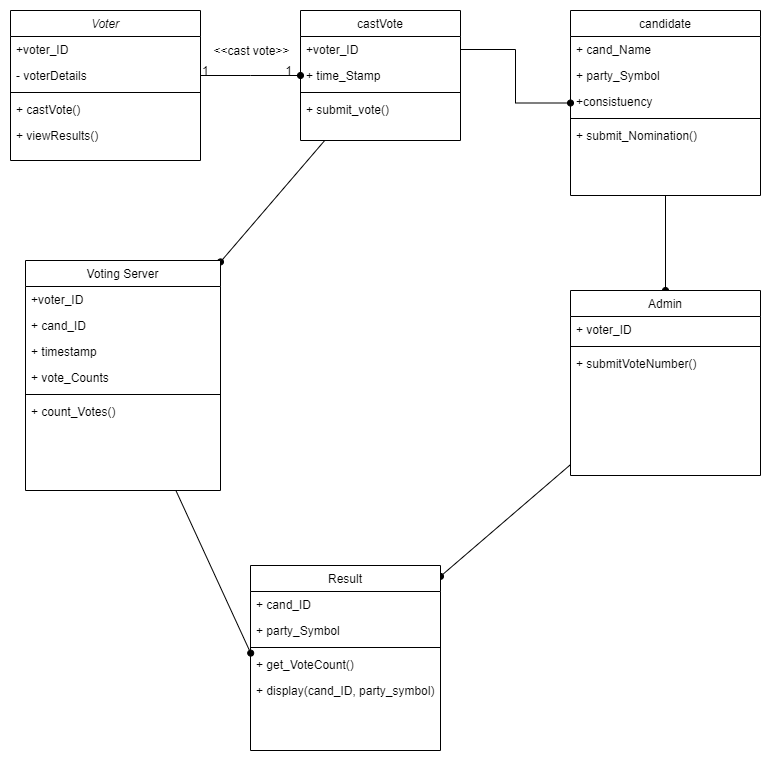
\includegraphics[width=\linewidth]{./Resources/class.png}
	\caption{Class Diagram}
	\label{fig:class}
\end{figure}
\newpage
\subsubsection{Sequence Diagram}
Sequence Diagrams are interaction diagrams that detail how operations are carried out. They capture the interaction between objects in the context of a collaboration. Sequence Diagrams are time focused and they show the order of the interaction visually by using the vertical axis of the diagram to represent time, what messages are sent and when.
\begin{figure}[H]
	\centering
	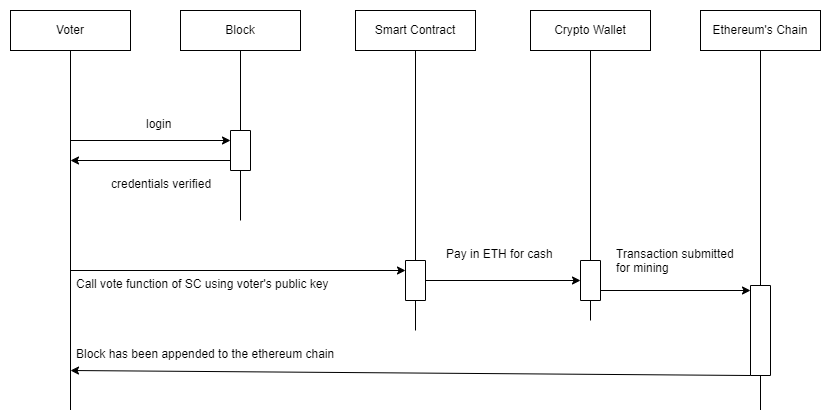
\includegraphics[width=\linewidth]{./Resources/sequence.png}
	\caption{SequenceDiagram}
	\label{fig:sequence}
\end{figure}
\newpage
\section{Project Implementation}
\newpage
\subsection{Module Description}
\begin{itemize}
	\item\textbf{Private Network}
	\\A blockchain private network, also known as a permissioned blockchain network, is a type of blockchain network that restricts access to participating nodes or entities. Unlike public blockchains, where anyone can join and participate, private blockchain networks are designed for specific organizations, consortia, or groups with predefined access controls.
	\\In a private blockchain network, the participating nodes are typically known and identified, and their permissions and roles within the network are predefined. This allows for more control and privacy compared to public blockchains, where all transactions and data are visible to the entire network.
	\\Private blockchain networks offer several advantages:
	\begin{enumerate}
		\item Enhanced privacy
		\item Increased scalability and efficiency
		\item Customized governance
		\item Reduced energy consumption
	\end{enumerate}
	Private blockchain networks are commonly used in industries such as finance, supply chain management, healthcare, and government, where data privacy, security, and controlled access are of utmost importance. These networks enable participants to collaborate, share data, and execute transactions securely and efficiently within a trusted ecosystem.
	\item\textbf{Smart Contract}
	\\A smart contract is a self-executing contract with predefined terms and conditions written in code. It is built on blockchain technology, most commonly associated with platforms like Ethereum, and allows for the automation and enforcement of agreements without the need for intermediaries.
	\\Smart contracts operate on the principle of "if-then" statements, where the terms of the contract are translated into lines of code. Once deployed on the blockchain, these contracts are immutable and execute automatically when certain predetermined conditions are met. This automation eliminates the need for intermediaries, such as lawyers or escrow agents, as the contract's execution is based on predefined rules and cannot be altered or tampered with.
	\newpage
	The key features of smart contracts include:
	\begin{enumerate}
		\item Autonomy
		\item Transparency
		\item Security
		\item Efficiency
	\end{enumerate}
	Smart contracts have a wide range of applications across various industries. They can be used for financial transactions, supply chain management, real estate transactions, intellectual property rights, voting systems, and more. By eliminating the need for intermediaries and relying on the security and transparency of blockchain technology, smart contracts offer a new level of efficiency and trust in conducting business and executing agreements.
	\item\textbf{Frontend}
	\\Frontend refers to the client-facing part of the website. It encompasses the user interface (UI) and user experience (UX) components that users interact with directly. The frontend is responsible for presenting data and functionality in a visually appealing and intuitive manner, enabling users to interact with the application or website effectively.
	\item\textbf{Synthetic Data}
	\\Synthetic data refers to artificially generated data that mimics the characteristics and statistical properties of real-world data. It is created using algorithms or models to simulate data patterns, distributions, and relationships found in actual datasets. Synthetic data is designed to maintain privacy and confidentiality by not containing any personally identifiable information (PII) or sensitive data.
\end{itemize}
\subsection{Tools and Technologies Used}
\begin{itemize}
	\item\textbf{Programming Languages}
	\begin{itemize}
		\item Solidity
		      \\Solidity is a programming language specifically designed for developing smart contracts on blockchain platforms, with Ethereum being the most popular one. It is a statically-typed, high-level language that enables developers to write code for executing smart contracts on the Ethereum Virtual Machine (EVM).
		\item JavaScript
		      \\JavaScript is a versatile and widely-used programming language primarily used for web development. It is a high-level, interpreted language that allows developers to add interactivity and dynamic behavior to websites. JavaScript can be executed on both the client side (in web browsers) and the server side (with the help of frameworks like Node.js).
		\item Python
		      \\Python is a high-level, interpreted programming language known for its simplicity, readability, and versatility. It was created by Guido van Rossum and first released in 1991. Python's design philosophy emphasizes code readability and a clean syntax, making it easier to write and understand compared to many other programming languages.
		      \\Python is widely used in various domains, including web development, scientific computing, data analysis, artificial intelligence, machine learning, automation, scripting, and more. Its versatility, readability, and extensive library support make it a popular choice for both beginners and experienced developers alike.
		\item TypeScript
		      \\TypeScript is a programming language developed by Microsoft that is a superset of JavaScript. It enhances JavaScript by adding optional static typing, which allows developers to catch errors and improve code quality during the development process. TypeScript code is translated into plain JavaScript and can be executed in any JavaScript runtime environment.
		\item HTML
		      \\HTML (Hypertext Markup Language) is the standard markup language used for creating the structure and content of web pages. It provides a set of tags (markup elements) that define the various components and elements of a web page. HTML is the backbone of the World Wide Web and is interpreted by web browsers to display web content.
		\item CSS
		      \\CSS (Cascading Style Sheets) is a style sheet language used to describe the presentation and visual appearance of web pages written in HTML and XML. It provides a set of rules that define how elements on a web page should be displayed, including their layout, colors, fonts, spacing, and other visual properties.
	\end{itemize}
	\item\textbf{Frameworks/Libraries/Packages}
	\begin{itemize}
		\item ReactJS (JavaScript)
		      \\ReactJS is a popular JavaScript library for building user interfaces (UIs) and creating interactive web applications. It was developed by Facebook and released in 2013. ReactJS follows a component-based architecture, where UIs are broken down into reusable and self-contained components that manage their own state and update efficiently.
		      \\ReactJS is widely used for building single-page applications, mobile applications (with React Native), and complex web interfaces. Its modular and efficient architecture, along with the vibrant community support, has made it a popular choice among developers for creating interactive and scalable UIs.
		\item Chai (JavaScript)
		      \\Chai is a popular assertion and expectation library for testing JavaScript code. It provides a clean and expressive syntax for making assertions about the behavior and expected outcomes of functions and code blocks. Chai can be used in various JavaScript environments, including browser-based applications and Node.js.
		      \\Chai provides a powerful and expressive way to write tests and make assertions about your JavaScript code's behavior. Its flexibility, wide range of assertions, and integration with popular testing frameworks make it a popular choice for JavaScript testing.
		\item Hardhat (JavaScript)
		      \\Hardhat is a development environment and task runner for building and testing Ethereum smart contracts and decentralized applications (DApps). It is designed to streamline the development workflow by providing a comprehensive set of tools and utilities specifically tailored for Ethereum development.
		      \\Hardhat has gained popularity among Ethereum developers due to its flexibility, extensibility, and comprehensive toolset. It simplifies the development and testing of Ethereum-based applications, making it an excellent choice for building and deploying smart contracts and DApps on the Ethereum blockchain.
		\item Web3 (Python)
		      \\Web3.py is a Python library that allows developers to interact with the Ethereum blockchain and build decentralized applications (DApps) using Python. It provides a convenient and user-friendly interface for working with Ethereum smart contracts, executing transactions, and interacting with blockchain data.
		      \\Web3.py is a powerful tool for Python developers interested in building Ethereum-based applications. It simplifies the process of interacting with the Ethereum blockchain and enables seamless integration with existing Python codebases, making it a popular choice for Ethereum development in the Python ecosystem.
		\item TailwindCSS (CSS)
		      \\Tailwind CSS is a highly customizable utility-first CSS framework that provides a comprehensive set of pre-built CSS classes for building user interfaces. Unlike traditional CSS frameworks that come with pre-designed components, Tailwind CSS focuses on providing low-level utility classes that can be combined to create custom designs and layouts.
		      \\Tailwind CSS is known for its simplicity, flexibility, and performance. By using utility classes as building blocks, developers have fine-grained control over the design and layout of their applications. It is particularly suitable for projects that require custom designs, rapid prototyping, or highly responsive interfaces.
	\end{itemize}
	\item\textbf{Ethereum Client}
	\\Geth, short for Go Ethereum, is one of the most widely used client implementations for the Ethereum blockchain. It is a command-line interface (CLI) tool and a full-featured Ethereum node written in the Go programming language. Geth allows users to interact with the Ethereum network, run their own Ethereum nodes, and deploy and execute smart contracts.
	\\Key features and functionalities of Geth include:
	\begin{enumerate}
		\item Ethereum Node
		\item Blockchain Synchronization
		\item Smart Contract Execution
		\item Ethereum Account Management
		\item Transaction Submission and Mining
		\item Network Configuration
		\item JSON-RPC API
		\item Developer Tools and Utilities
	\end{enumerate}
	Geth is a versatile and powerful tool for interacting with the Ethereum blockchain. It is used by developers, miners, and other participants in the Ethereum ecosystem to run their own Ethereum nodes, deploy smart contracts, interact with the network, and contribute to the decentralized nature of the Ethereum blockchain.
	\item\textbf{Ethereum Dashboard}
	\\Ethstats is a real-time network monitoring and statistics platform for Ethereum. The Ethstats dashboard provides an overview of key metrics and information about the Ethereum network, including block propagation, mining activity, network health, and other relevant statistics. It aims to provide users with insights into the performance and status of the Ethereum network.
	\newpage	
	The Ethstats dashboard offers various features and information, including:
	\begin{enumerate}
		\item Network Statistics
		\item Mining Information
		\item Block Propagation
		\item Network Health Indicators
		\item Peer Information
		\item Historical Data
		\item Customization and Filtering
	\end{enumerate}
	The Ethstats dashboard provides a comprehensive view of the Ethereum network, allowing users to monitor network health, mining activity, block propagation, and other critical metrics. It serves as a valuable tool for Ethereum stakeholders, developers, miners, and enthusiasts to gain insights into the performance and status of the Ethereum blockchain in real-time.
\end{itemize}
\subsection{Methodologies/Algorithm Details}
To implement and test a blockchain based voting system, a few components have to be designed. A privately hosted closed blockchain network is required for our contract to run on. This is created using ethereum’s Go language based client. To do so, a script is written in JavaScript to automate the following tasks :
\\\\\colorbox{gray!20}{%
	\begin{minipage}{\linewidth}%
		\vspace*{2pt}
		\begin{enumerate}
			\item Ethereum wallet accounts are created for the number of nodes required.
			\item On these accounts, the genesis block is initialized.
			\item Bootnode is initialized. Bootnode is a node which connects other nodes to each other.
			\item Geth (Go Ethereum Client) is run using the accounts created using bootnode initialized in the previous step.
		\end{enumerate}
		\vspace*{2pt}
	\end{minipage}%
}
\newpage
A Solidity based contract is written to execute the application’s core functionality. This contract works like the backend for the entire application. This contract is written in solidity version 0.8.19 :
\\\\\colorbox{gray!20}{%
	\begin{minipage}{\linewidth}%
		\vspace*{2pt}
		ElectoralContract \{
		\\\\\-\hspace{1cm}struct Voter \{
		\\\-\hspace{2cm}string voterName;
		\\\-\hspace{2cm}bool hasVoted;
		\\\-\hspace{2cm}bool isLoggedIn;
		\\\-\hspace{2cm}string voterPassword;
		\\\-\hspace{2cm}address nodeAddress;
		\\\-\hspace{2cm}uint timestamp;
		\\\-\hspace{1cm}\}
		\\\\\-\hspace{1cm}struct Candidate \{
		\\\-\hspace{2cm}string candidateName;
		\\\-\hspace{2cm}uint256 voteCount;
		\\\-\hspace{1cm}\}
		\\\\\-\hspace{1cm}// func addCandidate : adds candidate for voters to vote
		\\\-\hspace{1cm}// func addVoter : adds voter
		\\\-\hspace{1cm}// func login : login functionality for voter
		\\\-\hspace{1cm}// func logout : logout functionality for voter
		\\\-\hspace{1cm}// func getResult : gets result of elections
		\\\-\hspace{1cm}// func getCandidates : gets list of candidate names
		\\\-\hspace{1cm}// func getVotersDetailed : gets all voters information
		\\\-\hspace{1cm}// func vote : cast vote to candidate functionality
		\\\\\};
		\vspace*{2pt}
	\end{minipage}%
}
\\\\\\Algorithm to cast vote :
\\\\\colorbox{gray!20}{%
	\begin{minipage}{\linewidth}%
		\vspace*{2pt}
		\begin{table}[H]
			\resizebox{\textwidth}{!}{%
				\begin{tabular}{llll}
					Require & : & Voter must have not cast vote earlier &                                     \\
					Require & : & Voter must be logged in               &                                     \\
					Update  & : & candidate.voteCount++                 & //Update vote count for candidate   \\
					Update  & : & voter.hasVoted = true                 & //Update voting status for voter    \\
					Update  & : & voter.timestamp = timestamp           & //Update voting timestamp for voter \\
					Func    & : & logout(voterId)                       & //Logout voter
				\end{tabular}%
			}
		\end{table}
		\vspace*{2pt}
	\end{minipage}%
}
\newpage
The overall flow followed is :
\begin{figure}[H]
	\centering
	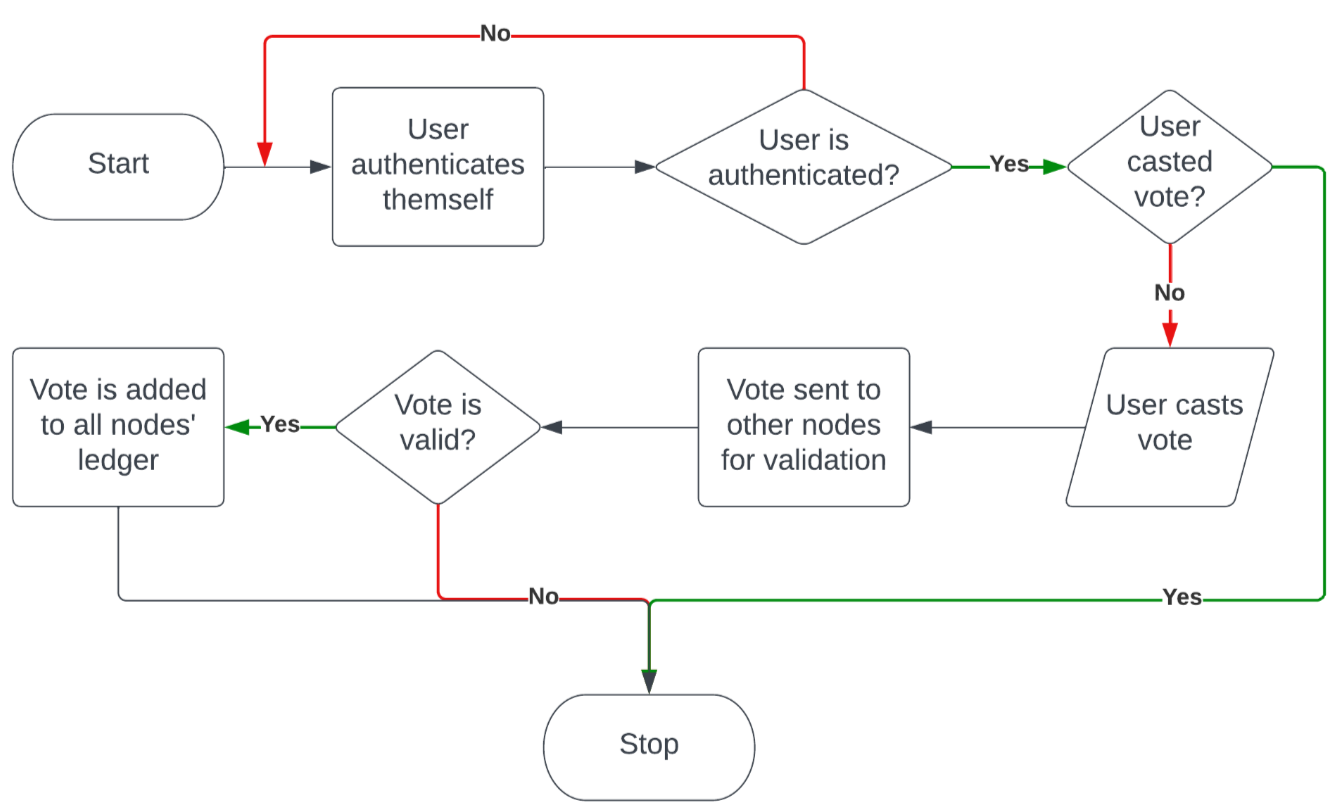
\includegraphics[width=\linewidth]{./Resources/flow.png}
	\caption{Flow of the system}
	\label{fig:flow}
\end{figure}
Consensus algorithm used in this chain is Proof of Authority (Clique). In PoA consensus, some nodes are given permission to generate new blocks. These nodes are called ‘Validators’. PoA leverages the importance of identities. The validators are not staking coins like PoS but rather their own reputation instead. PoA is suited for private networks such as this one.
\\\\Finally, to evaluate the system, some synthetic data is generated and provided to the system and performances tested. To perform this evaluation, python script is written which will perform these tasks :
\\\\\colorbox{gray!20}{%
	\begin{minipage}{\linewidth}%
		\vspace*{2pt}
		\begin{enumerate}
			\item Register a single candidate.
			\item Register required number of voters with random names.
			\item Login with all voters’ credentials.
			\item Cast votes by voters with preset probability.
			\item Logout all logged in voters.
			\item Get result and compile csv.
			\item Plot graphs from results.
		\end{enumerate}
		\vspace*{2pt}
	\end{minipage}%
}
\newpage
Along with these components, a frontend client is made for a citizen/voter to interact and cast their votes. Dashboards are also deployed to monitor the network and the data flowing through it. The system’s performance is tested by generating synthetic data which is passed to the system and the time taken for it to process the data and store it in blockchain. The number of nodes in the system are scaled in range from 1 to 50 while ranging the voters from 10 to 250.
\subsection{Verification and Validation}
Table \ref{tab:result-table} shows time taken in seconds by the system to insert data to the private blockchain network and generate results without artificial delay included.
\begin{table}[H]
	\resizebox{\textwidth}{!}{%
		\begin{tabular}{|cr|rrrrrrrrrr|}
			\hline
			\multicolumn{2}{|c|}{\multirow{2}{*}{}} & \multicolumn{10}{c|}{Number of nodes}                                                                                                                                                                                                                                                                                      \\ \cline{3-12}
			\multicolumn{2}{|c|}{}                  & \multicolumn{1}{r|}{1}                & \multicolumn{1}{r|}{2}     & \multicolumn{1}{r|}{3}      & \multicolumn{1}{r|}{4}     & \multicolumn{1}{r|}{5}      & \multicolumn{1}{r|}{10}     & \multicolumn{1}{r|}{15}     & \multicolumn{1}{r|}{20}     & \multicolumn{1}{r|}{25}     & 50                                   \\ \hline
			\multicolumn{1}{|c|}{\multirow{4}{*}{}} & 10                                    & \multicolumn{1}{r|}{0.46}  & \multicolumn{1}{r|}{7.08}   & \multicolumn{1}{r|}{2.4}   & \multicolumn{1}{r|}{5.89}   & \multicolumn{1}{r|}{20.26}  & \multicolumn{1}{r|}{6.27}   & \multicolumn{1}{r|}{6.76}   & \multicolumn{1}{r|}{10.15}  & \multicolumn{1}{r|}{5.94}   & 4.84   \\ \cline{2-12}
			\multicolumn{1}{|c|}{}                  & 20                                    & \multicolumn{1}{r|}{0.9}   & \multicolumn{1}{r|}{13.56}  & \multicolumn{1}{r|}{3.75}  & \multicolumn{1}{r|}{5.97}   & \multicolumn{1}{r|}{35.4}   & \multicolumn{1}{r|}{13.16}  & \multicolumn{1}{r|}{17.4}   & \multicolumn{1}{r|}{14.87}  & \multicolumn{1}{r|}{12.44}  & 56.11  \\ \cline{2-12}
			\multicolumn{1}{|c|}{}                  & 30                                    & \multicolumn{1}{r|}{1.33}  & \multicolumn{1}{r|}{19.15}  & \multicolumn{1}{r|}{6.16}  & \multicolumn{1}{r|}{10.16}  & \multicolumn{1}{r|}{45.24}  & \multicolumn{1}{r|}{81.77}  & \multicolumn{1}{r|}{22.4}   & \multicolumn{1}{r|}{19.29}  & \multicolumn{1}{r|}{19.11}  & 41.7   \\ \cline{2-12}
			\multicolumn{1}{|c|}{}                  & 40                                    & \multicolumn{1}{r|}{1.76}  & \multicolumn{1}{r|}{8.88}   & \multicolumn{1}{r|}{9.25}  & \multicolumn{1}{r|}{13.58}  & \multicolumn{1}{r|}{61}     & \multicolumn{1}{r|}{31.21}  & \multicolumn{1}{r|}{30.11}  & \multicolumn{1}{r|}{31.57}  & \multicolumn{1}{r|}{29.68}  & 33.01  \\ \cline{2-12}
			\multicolumn{1}{|c|}{Voters}            & 50                                    & \multicolumn{1}{r|}{2.3}   & \multicolumn{1}{r|}{35.77}  & \multicolumn{1}{r|}{11.73} & \multicolumn{1}{r|}{15}     & \multicolumn{1}{r|}{65.16}  & \multicolumn{1}{r|}{43.83}  & \multicolumn{1}{r|}{39.35}  & \multicolumn{1}{r|}{37.42}  & \multicolumn{1}{r|}{32.23}  & 28.8   \\ \cline{2-12}
			\multicolumn{1}{|c|}{\multirow{4}{*}{}} & 100                                   & \multicolumn{1}{r|}{4.61}  & \multicolumn{1}{r|}{22.82}  & \multicolumn{1}{r|}{21.81} & \multicolumn{1}{r|}{30.53}  & \multicolumn{1}{r|}{139.74} & \multicolumn{1}{r|}{87.84}  & \multicolumn{1}{r|}{71.14}  & \multicolumn{1}{r|}{77.71}  & \multicolumn{1}{r|}{70.99}  & 111.91 \\ \cline{2-12}
			\multicolumn{1}{|c|}{}                  & 150                                   & \multicolumn{1}{r|}{7.93}  & \multicolumn{1}{r|}{35.41}  & \multicolumn{1}{r|}{34.93} & \multicolumn{1}{r|}{45.02}  & \multicolumn{1}{r|}{166.75} & \multicolumn{1}{r|}{100.94} & \multicolumn{1}{r|}{113.08} & \multicolumn{1}{r|}{112.71} & \multicolumn{1}{r|}{111.59} & 161.79 \\ \cline{2-12}
			\multicolumn{1}{|c|}{}                  & 200                                   & \multicolumn{1}{r|}{11.18} & \multicolumn{1}{r|}{49.99}  & \multicolumn{1}{r|}{46.33} & \multicolumn{1}{r|}{72.57}  & \multicolumn{1}{r|}{-}      & \multicolumn{1}{r|}{167.5}  & \multicolumn{1}{r|}{143.24} & \multicolumn{1}{r|}{164.77} & \multicolumn{1}{r|}{155}    & 273.67 \\ \cline{2-12}
			\multicolumn{1}{|c|}{}                  & 250                                   & \multicolumn{1}{r|}{13.34} & \multicolumn{1}{r|}{152.75} & \multicolumn{1}{r|}{59.7}  & \multicolumn{1}{r|}{105.66} & \multicolumn{1}{r|}{-}      & \multicolumn{1}{r|}{191.49} & \multicolumn{1}{r|}{169.56} & \multicolumn{1}{r|}{189.36} & \multicolumn{1}{r|}{184.24} & 209.19 \\ \hline
		\end{tabular}%
	}
	\caption{Time Taken - (Number Of Nodes Vs Voters)}
	\label{tab:result-table}
\end{table}
During evaluation of the system, we faced many failures due to block creation taking a long time, blockchain not being synchronized properly across the network, running out of resources for mining and some unexpected system crashes. Due to these crashes, results for 5 nodes, 200 and 250 voters could not be obtained.
\newpage
\section{Software Testing}
\newpage
\subsection{Test Plan}
Software testing is an activity that helps in finding out bugs/defects/errors in a software system under development, in order to provide a bug free and reliable system/solution to the customer. Testing of software is always carried out in two parts viz.. Verification and validation. Verification refers to the set of activities that ensure that software correctly implements a specific function. Validation refers to a different set of activities that ensure that the software has been built is traceable to customer requirements.
\\\\Software scope describes the functions and features that are to be delivered to end users, the data that are input and output, and the content that is presented to the users as consequence of using the software. Test plan for this project involves the testing of the individual components for modules interface.
\\\\The software is tested using two levels of testing viz. black box testing and white box testing. White box testing could be carried out in three different phases viz. unit testing system/ integration testing and validation testing.
\subsection{Test Cases and Test Result}
\subsubsection{Smoke Testing}
Whenever a new build is provided by the development team then the software testing team validates the build and ensures that no major issue exists. The testing team ensures that the build is stable and a detailed level of testing is carried out further. Smoke Testing checks that no show stopper defect exists in the build which will prevent the testing team to test the application in detail. If testers find that the major critical functionality is broken down at the initial stage itself then testing team can reject the build and inform accordingly to the development team. Smoke Testing is carried out to a detailed level of any functional or regression testing.
\subsubsection{Sanity Testing}
Sanity Testing is done to determine if a new software version is performing well enough to accept it for a major testing effort or not. If an application is crashing for the initial use then the system is not stable enough for further testing. Hence a build or an application is assigned to fix it.
\subsubsection{Unit Testing}
Unit Testing, also known as Module Testing, focuses verification efforts on the module. The module is tested separately and this is carried out at the programming stage itself. Unit Test comprises the set of tests performed by an individual programmer before integration of the unit into the system. Unit test focuses on the smallest unit of software design- the software component or module.
\subsubsection{Integration Testing}
It is a systematic technique for constructing the program structure while at the same time conducting tests to uncover errors associated with the interface. It takes the unit tested modules and builds a program structure. All the modules are combined and tested as a whole. Integration of all the components to form the entire system and an overall testing is executed.
\subsubsection{Regression Testing}
Testing an application as a whole for the modification in any module or functionality is termed as Regression Testing. It is difficult to cover all the systems in Regression Testing, so typically automation testing tools are used for these types of testing.
\subsubsection{Validation Testing}
Validation tests succeed when the software functions in a manner that can be reasonably expected by the client. Software validation is achieved through a series of black box testing which confirms the requirements. Black box testing is conducted at the software interfaces. The test is designed to uncover interface errors, is also used to demonstrate that software functions are operational, input is properly accepted, output is produced, and that the integrity of external information is maintained. Both the plan and procedure are designed to ensure that all functional requirements are satisfied, all behavioral characteristics are achieved, all performance requirements are attained, documentation is correct, and human engineered, and other requirements are met.
\subsubsection{System Testing}
Tests to find the discrepancies between the system and its original objective, current specifications and system documentation. The system software is tested as a whole. It verifies all elements mesh properly to make sure that all system functions and performance are achieved in the target environment.
\\\\The focus areas are:
\begin{itemize}
	\item System functions and performance.
	\item System reliability and recoverability (recovery test).
	\item System behavior in the special conditions (stress and load test).
	\item System user operations (acceptance test/alpha test).
	\item Hardware and software integration collaboration.
	\item Integration of external software and the system.
\end{itemize}
\subsubsection{Output Testing}
Output of test cases compared with the expected results during design of test cases. Asking the user about the format required by them tests the output generated or displayed by the system under consideration. Here, the output format is considered into two ways, one is on screen and another one is printed format.
\\\\The output on the screen is found to be correct as the format was designed in the system design phase according to user needs. The output comes out as the specified requirements as the user’s hardcopy.
\subsubsection{Performance Testing}
Performance testing determines the amount of execution time spent in various parts of the unit, program throughput, and the response time and device utilization of the program unit. It occurs throughout all steps in the testing process.
\subsubsection{GUI Testing}
Graphical User Interface (GUIs) present interesting challenges for software engineers. Because of reusable components provided as part of GUI development environments, the creation of the user interface has become less time consuming and more precise.
\newpage
\section{Screenshots}
\newpage
\begin{figure}[H]
	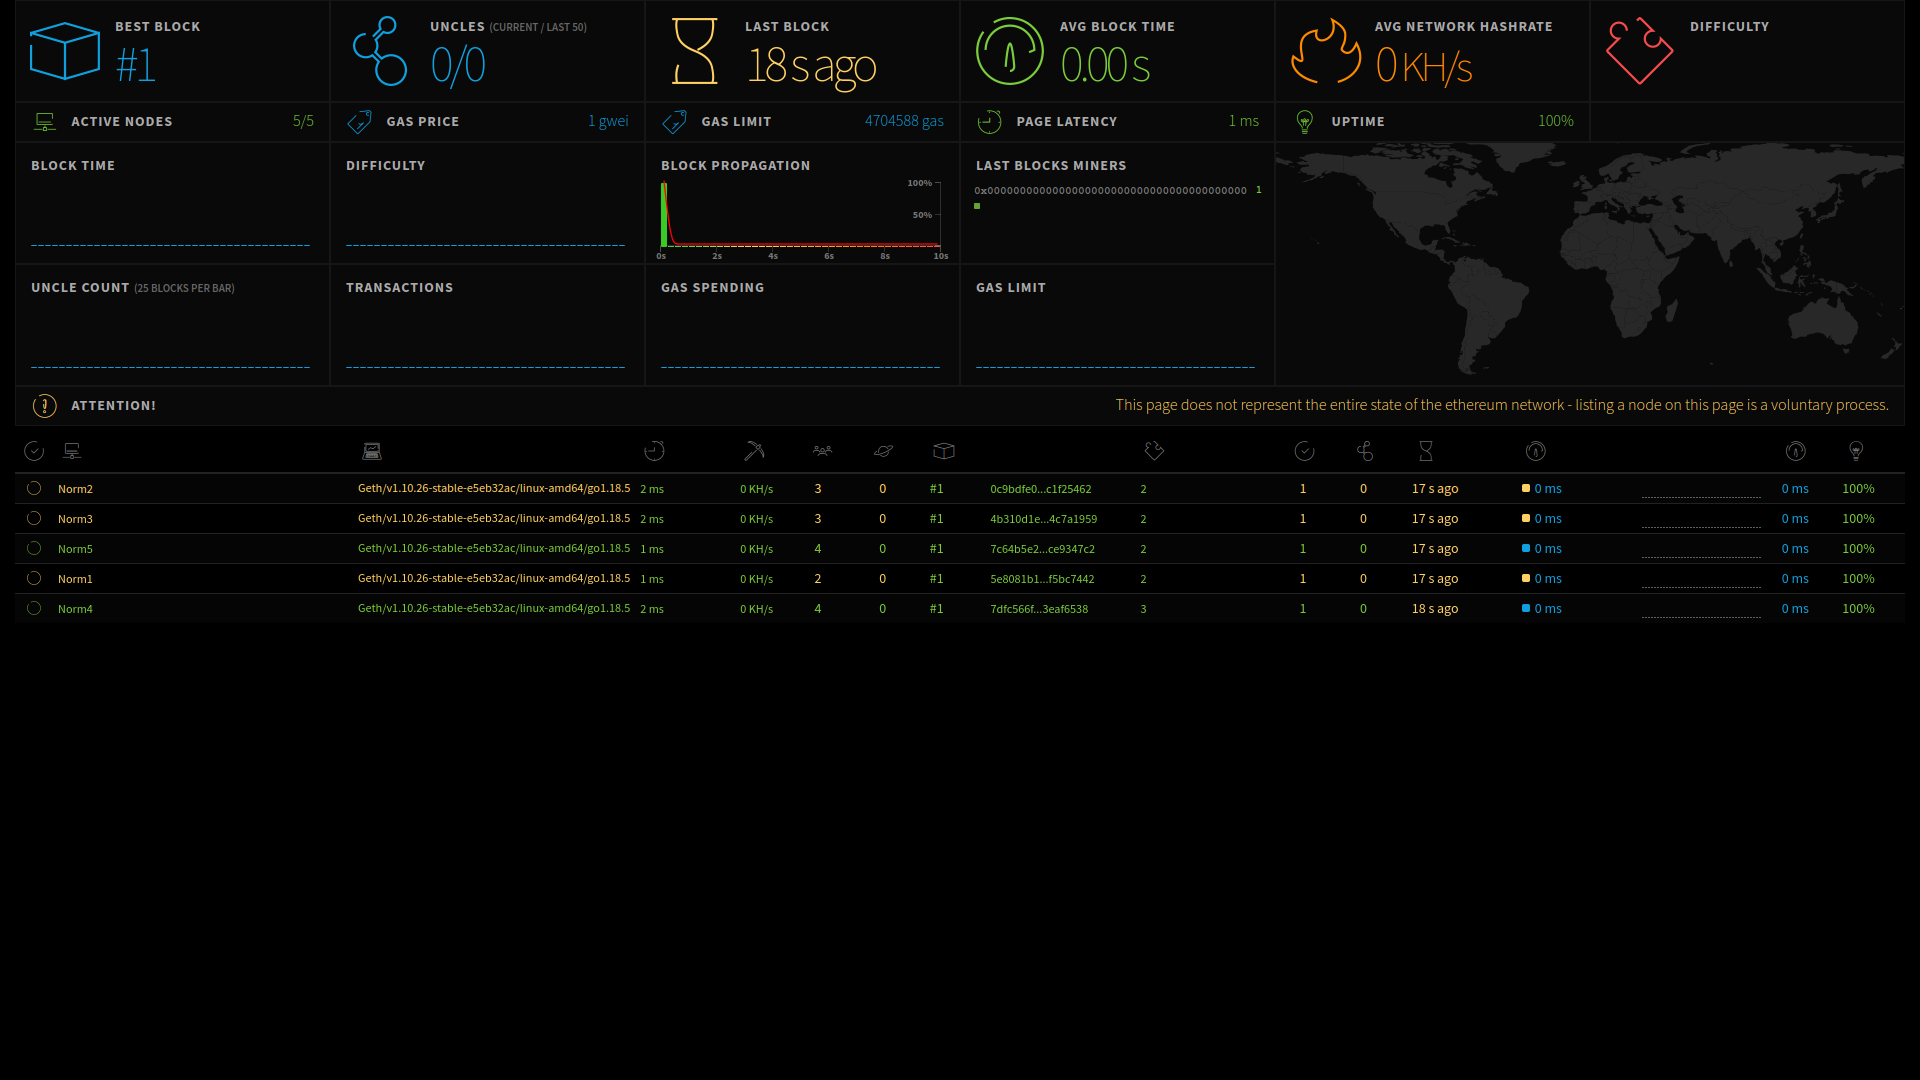
\includegraphics[width=\linewidth]{./Resources/ethstats.png}
	\caption{Ethstats}
	\label{fig:ethstats}
\end{figure}
\begin{figure}[H]
	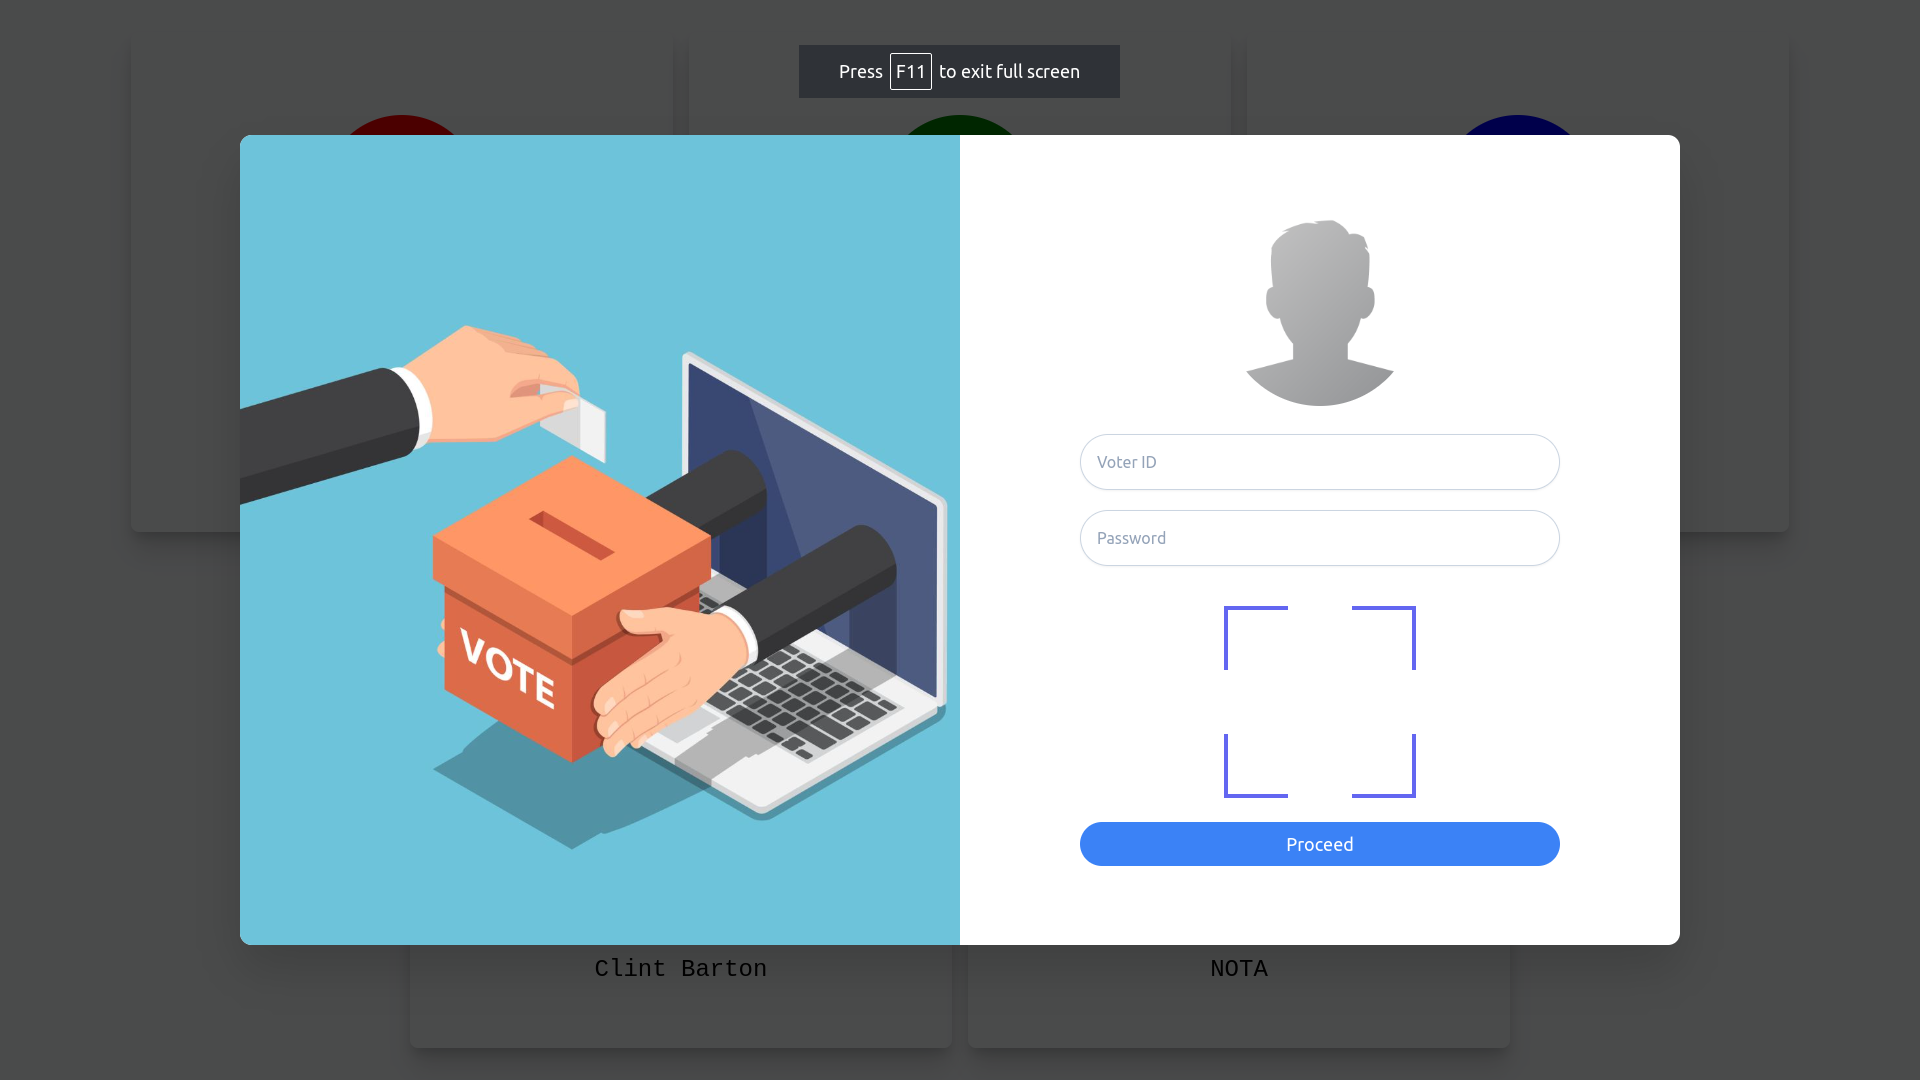
\includegraphics[width=\linewidth]{./Resources/login.png}
	\caption{Login}
	\label{fig:login}
\end{figure}
\begin{figure}[H]
	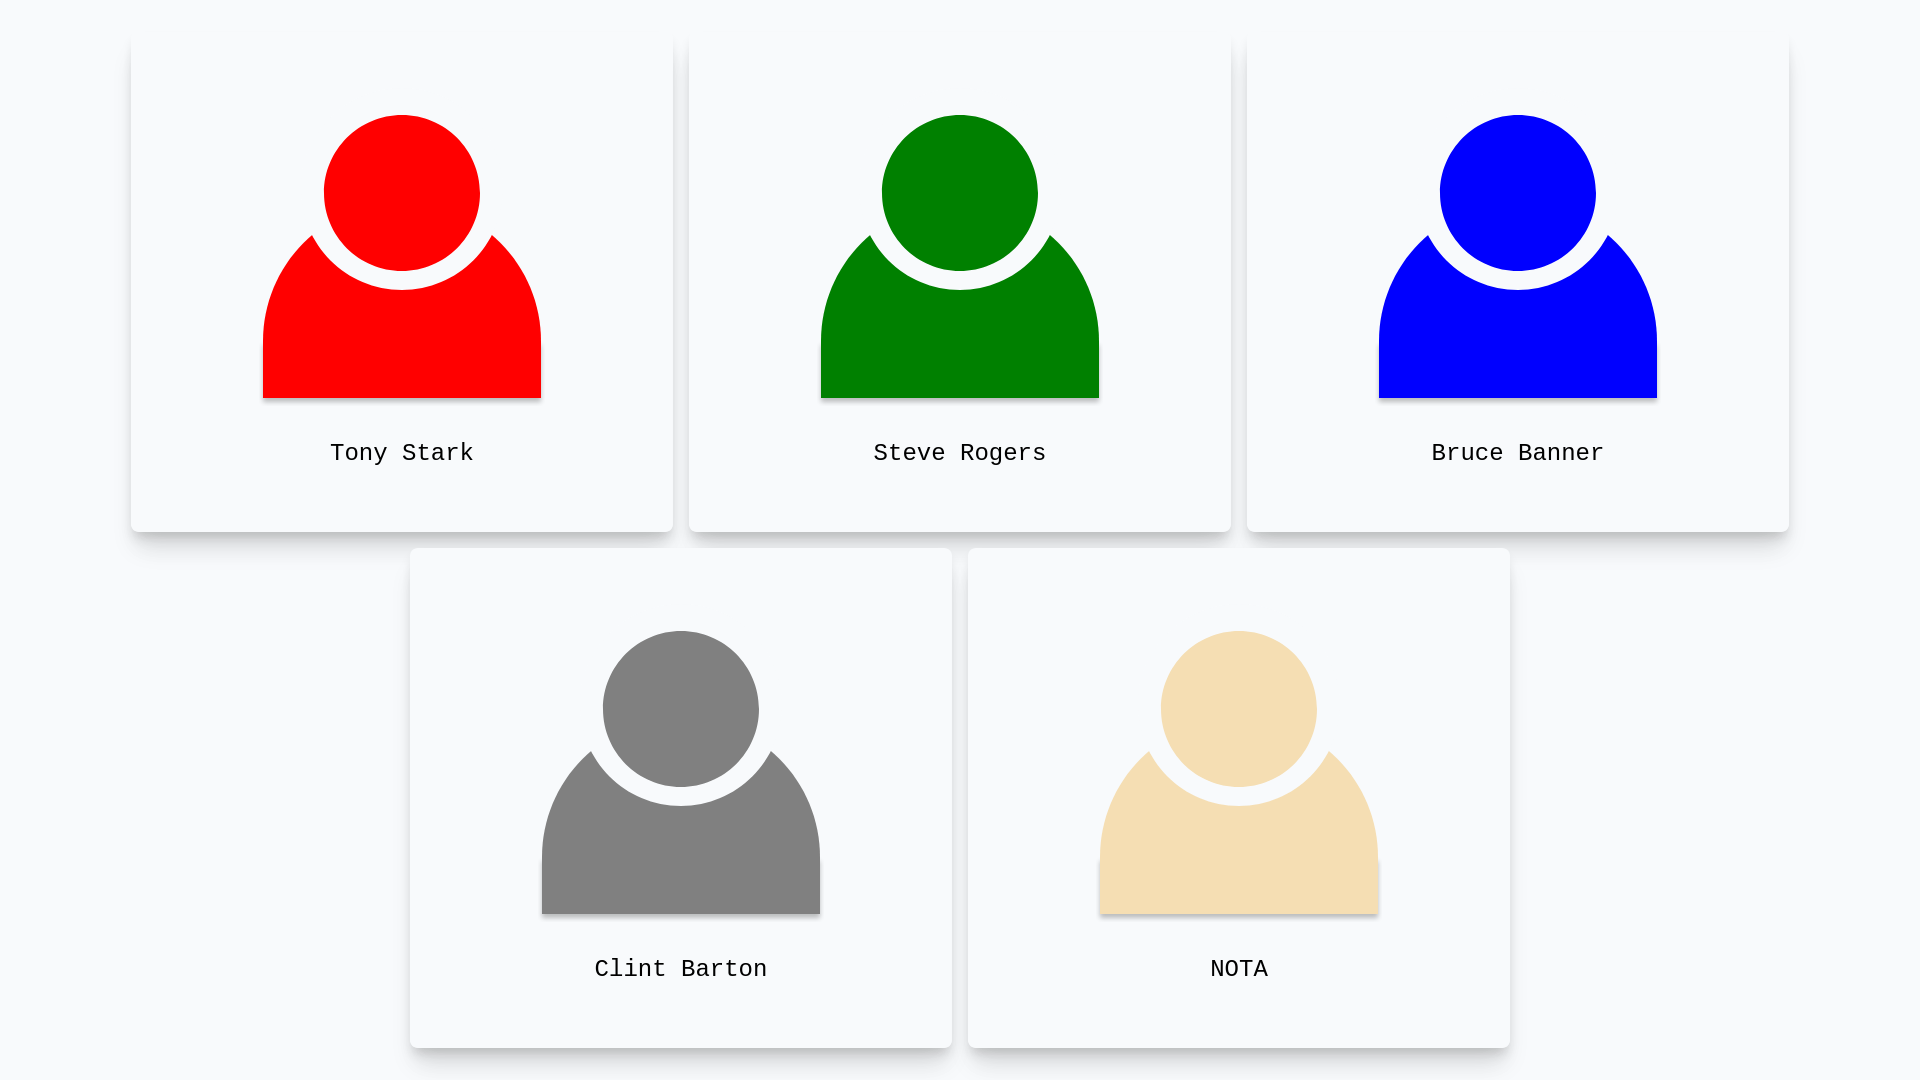
\includegraphics[width=\linewidth]{./Resources/pre-vote.png}
	\caption{Before selecting candidate}
	\label{fig:pre-vote}
\end{figure}
\begin{figure}[H]
	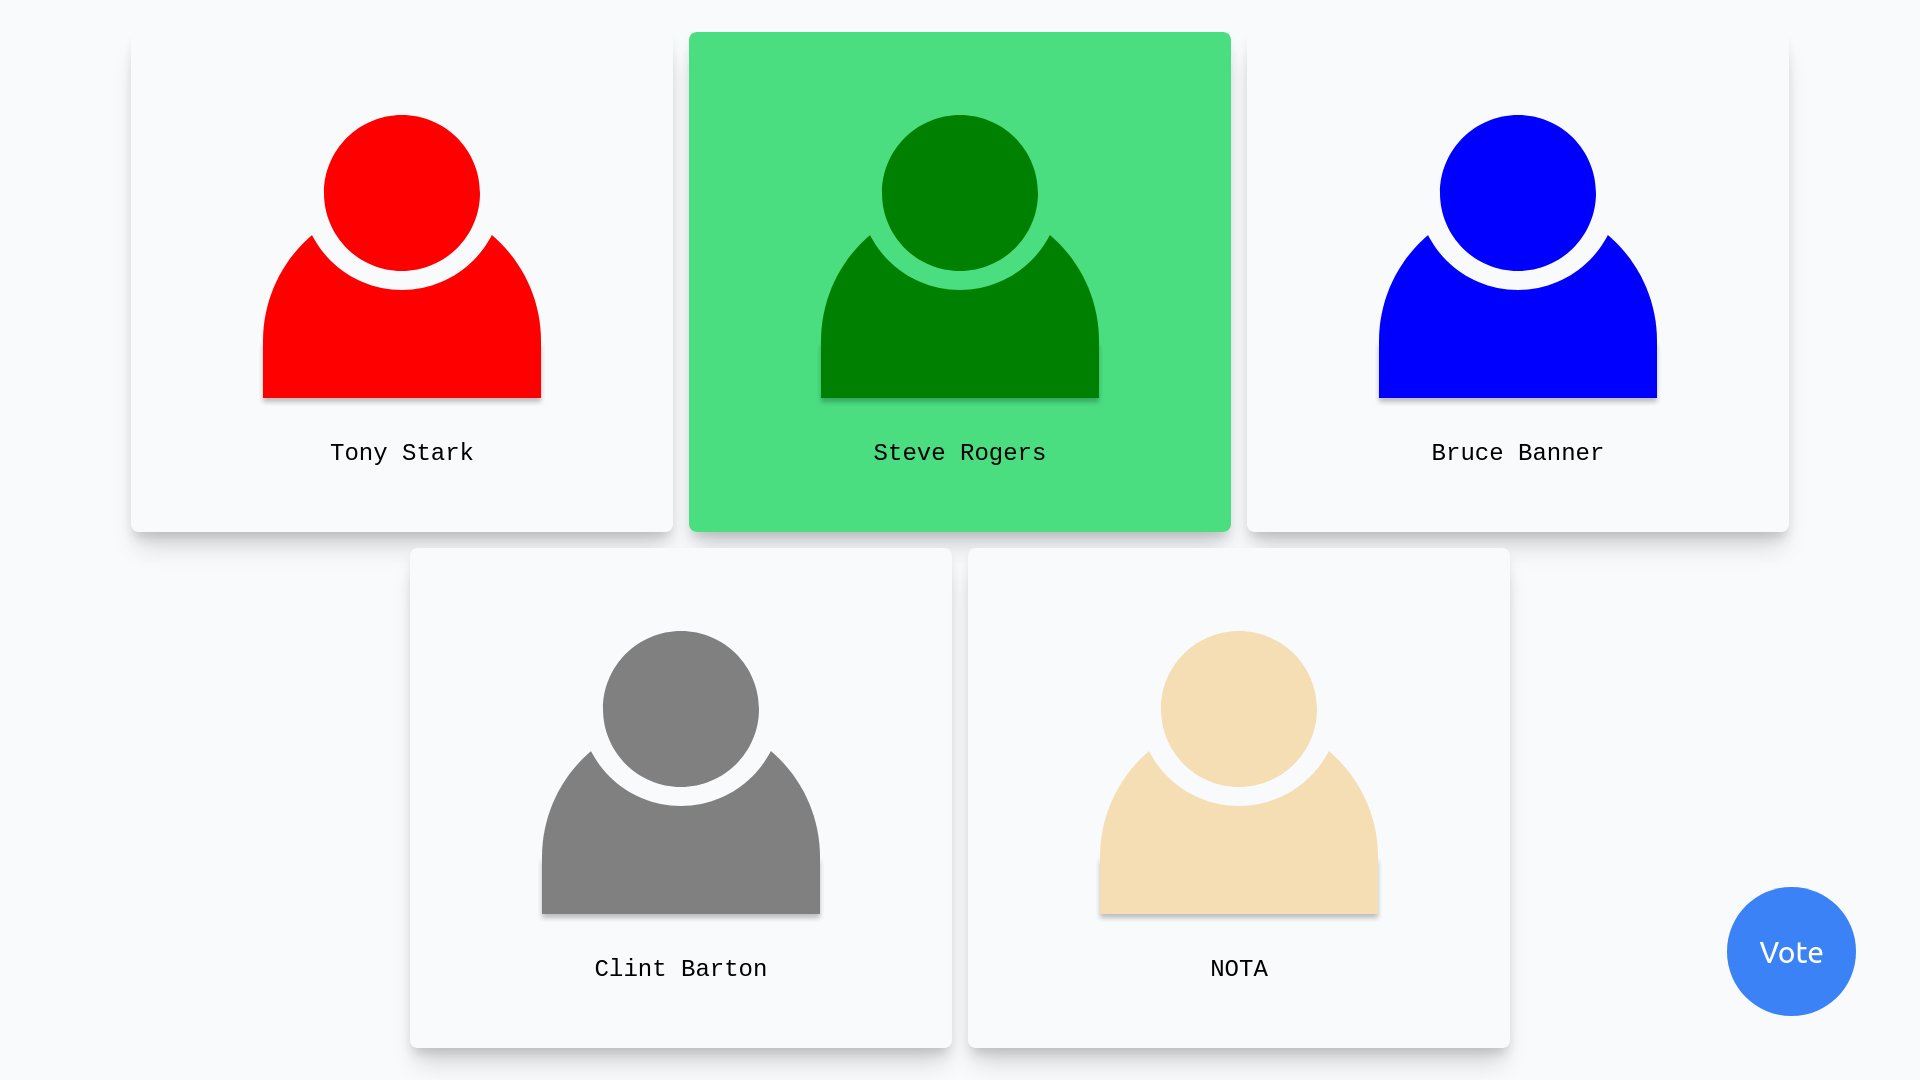
\includegraphics[width=\linewidth]{./Resources/post-vote.png}
	\caption{After selecting candidate}
	\label{fig:post-vote}
\end{figure}
\begin{figure}[H]
	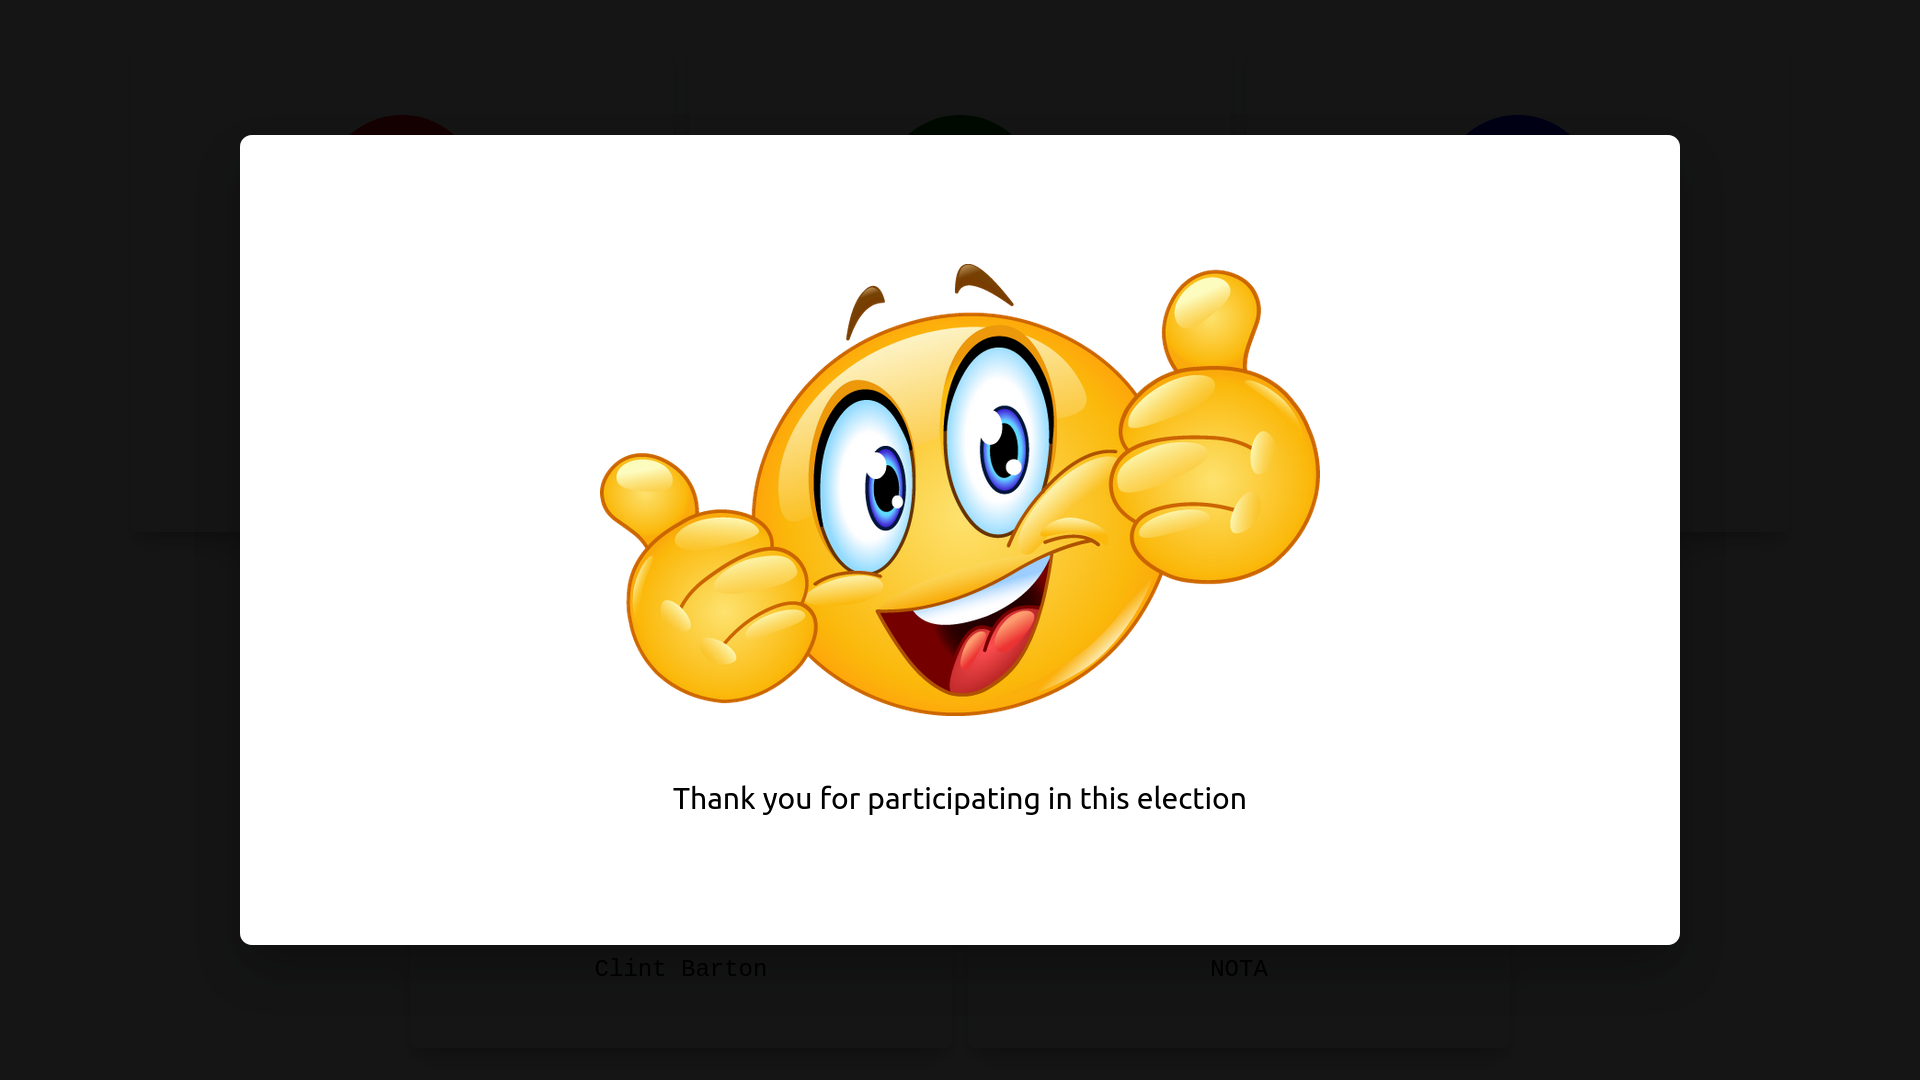
\includegraphics[width=\linewidth]{./Resources/thankyou.png}
	\caption{After casting vote}
	\label{fig:thankyou}
\end{figure}
\begin{figure}[H]
	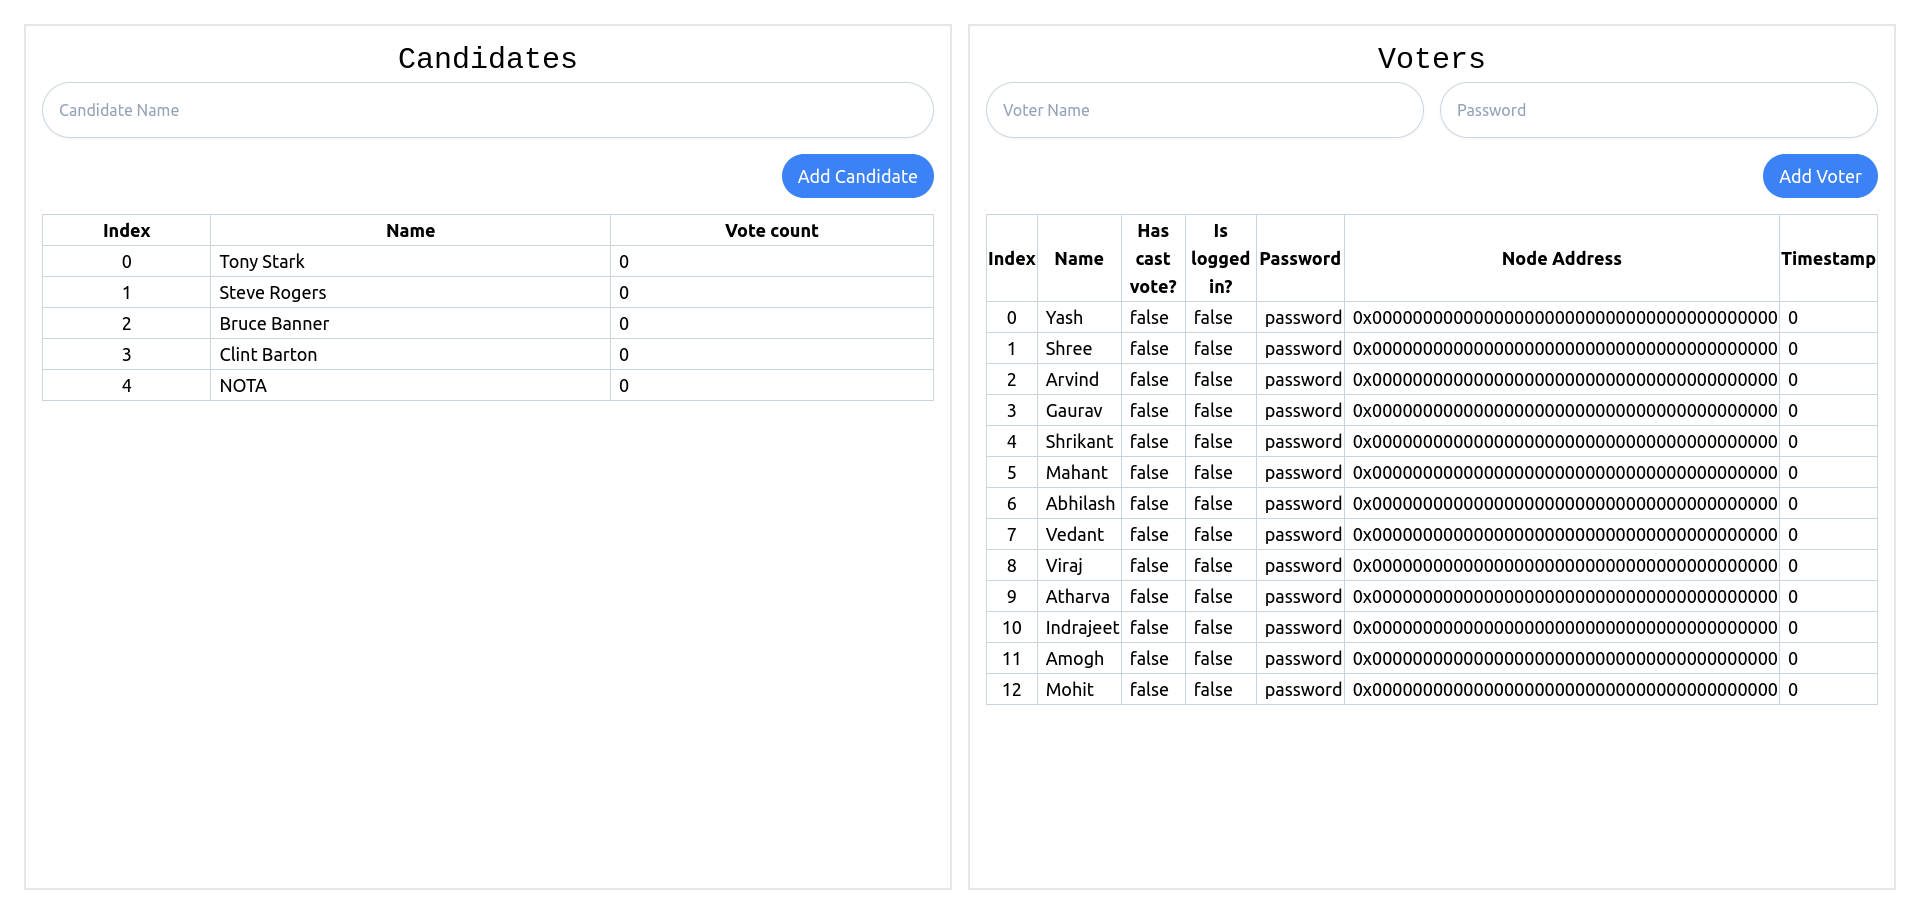
\includegraphics[width=\linewidth]{./Resources/admin.png}
	\caption{Admin Dashboard}
	\label{fig:admin}
\end{figure}
\newpage
\section{Deployment and Maintenance}
\newpage
\subsection{Deployment}
\begin{itemize}
	\item When the system meets approval and is ready to go live, we deploy it to the production environment and assist the transition to the new system.
	\item The development platforms we use support a broad range of deploymentoptions.
	\item There is no need to install any software on end-users’ machine since we plan to convert this application into executable file format.
\end{itemize}
\subsection{Maintenance}
\begin{itemize}
	\item Systems evolve after deployment. We will continue to make improvements and changes to our system as needed.
	\item With Survey, delivering the latest revisions to the users will be our priority, and will be completely transparent to the users.
	\item We can also train the user to maintain the system.
\end{itemize}
\newpage
\section{Conclusion and Future Scope}
\newpage
\subsection{Conclusion}
Through the numerous trial runs and performance testing, we were able to make a few observations. These observations were made based on the performance table in the Result section and self experiences while evaluating the system.
\begin{enumerate}
	\item As the number of voters increases a gradual increase is observed in time taken to insert transactions and get results.
	\item The time taken also increases as the number of nodes in the system is increased. This is due to blockchain synchronization across the network.
	\item Less number of nodes showed instability and frequent crashes since load not being distributed well enough. As the nodes increased, the stability increased and less crashes were observed.
\end{enumerate}
From the observations, we can say that voting using blockchain technology is feasible and will be beneficial due to its security and distributed nature. Since voting is carried on large scales, it will be stable and solve few issues faced by the current voting system.
\subsection{Future Scope}
To improve accuracy we need to increase the number of nodes. Increasing the number of nodes also affects the speed of the system but increases security. Balancing all these characteristics and producing results in optimal time would be the aim of the system in future. Also hardware resource optimization is also the aim. It makes the blockchain environment friendly and causes less harm to the environment. Moreover hardware optimization helps to include nodes with medium to less computing capacity to participate in mining. This increases miners and  would help the spread of the chain.
\newpage
\section{References}
\newpage
\bibliographystyle{ieeetr}
\bibliography{References}
\newpage
\section{Annexure A:\\Laboratory Assignments on Project Analysis of Algorithmic Design}
\newpage
\subsection{Introduction}
Blockchain technology can be used in the E-voting system to conduct a fair election and reduce injustice. The physical voting systems have many flaws in it as well as the digital voting systems are not perfect enough to be implemented on a large scale. This paper presents an overview of Blockchain based voting systems. The proposed platform will provide a framework that can be implemented to conduct voting activity digitally through blockchain. Our proposed system will use a flexible blockchain with consensus algorithms. The Chain security algorithm used in makes voting transactions more secure and integrated.
\\\textbf{Blockchain:} Blockchain is like a distributed ledger technology consisting of records of transactions called as blocks that are linked together using mathematical cryptography. Blockchain technology is popular because of its distributed nature which makes it immutable and practically impossible to hack.
\\\textbf{Distributed Ledger:} Ledger is a records collection containing information about transactions. Distributed ledger is a data structure capable of storing said transactions which is distributed across different computers on the network. DLT (Distributed Ledger Technology) is technology that distributes transaction records to all the users participating in the network. Blockchain is a type of Distributed Ledger Technology(DLT). Hence the data is shared among all its users providing transparency and preventing corruption.
\\\textbf{Decentralized Application(dApp):} dApp is an application built to run on decentralized computing, blockchain or any other distributed ledger system. It makes use of smart contracts for its functioning.
\\\textbf{Smart Contract:} Smart contracts are computer programs that automatically execute or control actions according to the terms of a contract or an agreement. It is used to enforce rules in blockchain transactions. Smart contracts are considered fundamental building blocks for cryptocurrencies and NFTs.
\\\textbf{Consensus:} Consensus ensures that all the different users participating in blockchain come to a mutual agreement regarding the state of blockchain. There are numerous consensus mechanisms that are used by different blockchain applications.
\\\textbf{Cryptography:} Cryptography is based on mathematical theory and computer science. Cryptography’s importance is to provide methods to secure and protect data and communications using encryption related techniques.
\\\textbf{Ethereum:} Ethereum is an open-source blockchain which provides smart contract functionality using solidity programming language.
\newpage
\subsection{Motivation}
India is said to have the largest democracy. For the electoral voting system India is using modern “Electronic Voting Machines” which are responsible for taking user input and storing the votes entered by the end user. Later these votes are carried to a central location where they are counted and the result is declared. Though, there is a possibility that these votes data can be tampered with. Having a single central server to store data creates a single point of failure for the entire system. These issues cause mistrust regarding the current system. In the traditional ballot paper system, vote authenticity was questionable and had its separate issues for which it was replaced with modern Electronic Voting Machines. Blockchain is based on Distributed Ledger Technology(DLT). In DLT, replicas of the same data are made on different nodes in the network due to which there is no single point of failure. Moreover, due to consensus algorithms implemented in blockchain, all nodes decide and agree upon whether a block is valid and must be added to the network or not.
\\\\Using Blockchain Technology will overcome issues in the present electronic voting system. It will also contribute to increasing the overall trust in the system and benefit democracy. Blockchain will provide a secure system for vote acceptance, storage and provide faster election results.
\subsection{Objective}
To design a decentralized e-voting system that,
\begin{enumerate}
	\item Reduces human interaction in the process of voting and elections in general.
	\item Does not depend on a trusted third party for controlling the collected data, whilst still staying immune to attacks and guaranteeing user privacy.
	\item Provides transparency, ensuring security and does not jeopardize voter privacy.
\end{enumerate}
\subsection{Architectural Design}
\begin{figure}[H]
	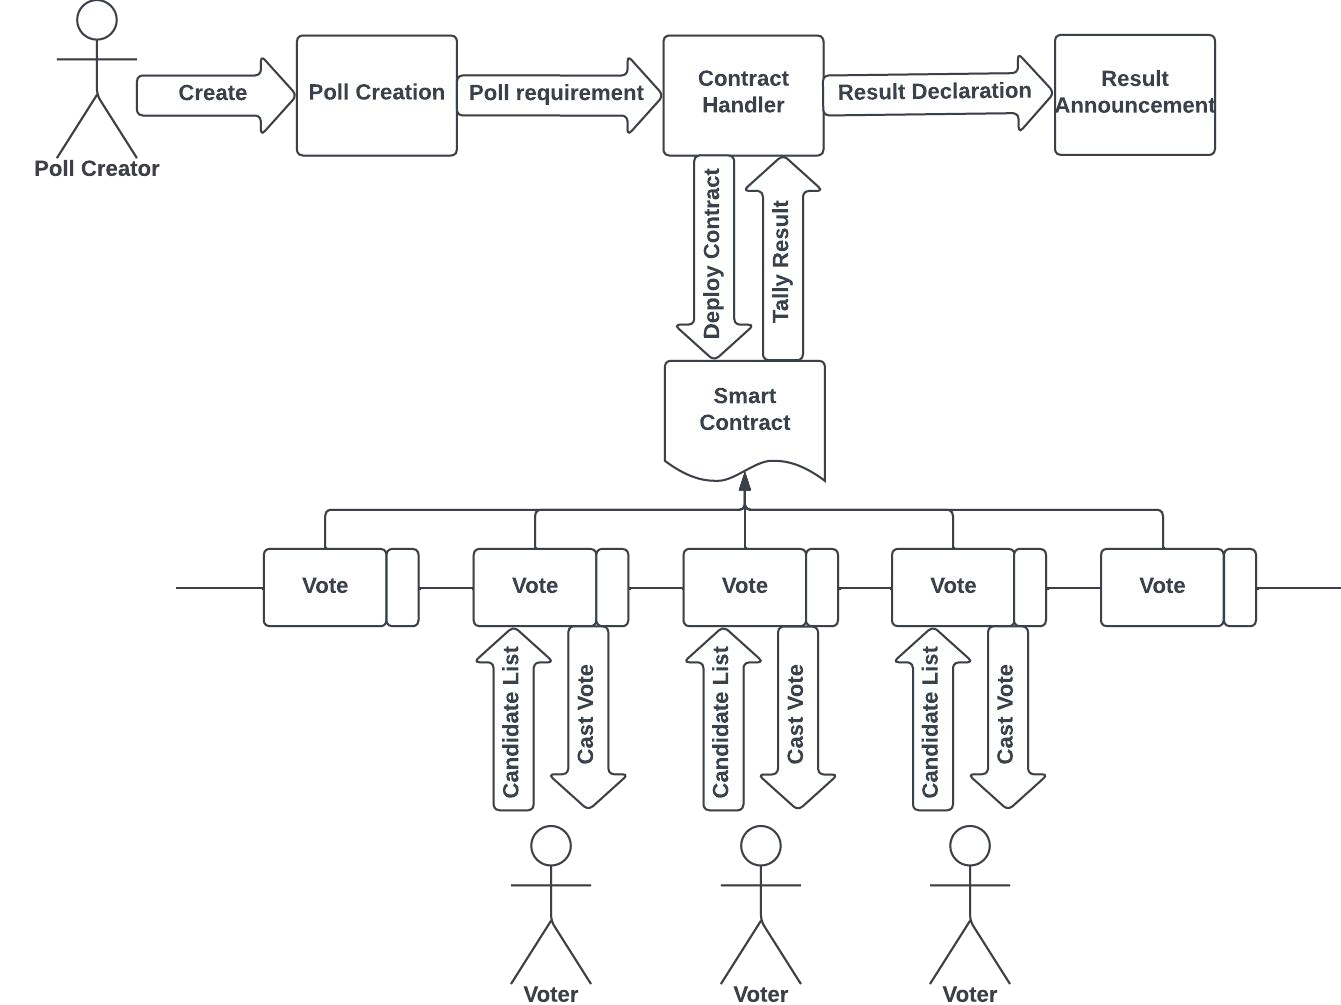
\includegraphics[width=\linewidth]{./Resources/architecture.png}
	\caption{Blockchain based e-Voting Architecture}
	\label{fig:annexure-architecture}
\end{figure}
\newpage
\section{Annexure B:\\Project Planner}
\newpage
\begin{table}[]
	\centering
	\begin{tabular}{|c|l|c|c|}
		\hline
		SR.NO. & TASK NAME                                                                          & DURATION & COMPLETION \\ \hline
		1      & Topic searching                                                                    & 15 days  & C          \\ \hline
		2      & Topic selection                                                                    & 10 days  & C          \\ \hline
		3      & Project Confirmation                                                               & 5 days   & C          \\ \hline
		4      & Literature Survey                                                                  & 15 days  & C          \\ \hline
		5      & Requirement Analysis                                                               & 15 day   & C          \\ \hline
		6      & Survey paper                                                                       & 10 days  & C          \\ \hline
		7      & Network Creation                                                                   & 10 days  & C          \\ \hline
		8      & \begin{tabular}[c]{@{}l@{}}Creation of Blockchain and\\ Genesis Block\end{tabular} & 10 days  & C          \\ \hline
		9      & \begin{tabular}[c]{@{}l@{}}Implementation of Solidity\\ Contracts\end{tabular}     & 2 weeks  & C          \\ \hline
		10     & \begin{tabular}[c]{@{}l@{}}Implementation of Front End\\ using React\end{tabular}  & 3 weeks  & C          \\ \hline
		11     & \begin{tabular}[c]{@{}l@{}}Optimization and Performance\\ Evaluation\end{tabular}  & 3 weeks  & C          \\ \hline
		12     & Code Integration and testing                                                       & 2 weeks  & C          \\ \hline
		13     & Implementation Paper Publishing                                                    & 2 weeks  & C          \\ \hline
		14     & Documentation                                                                      & 10 days  & C          \\ \hline
	\end{tabular}
	\caption{System Implementation Plan}
	\label{tab:system-implementation-plan}
\end{table}
\newpage
\section{Annexure C:\\Plagiarism Report}
\newpage
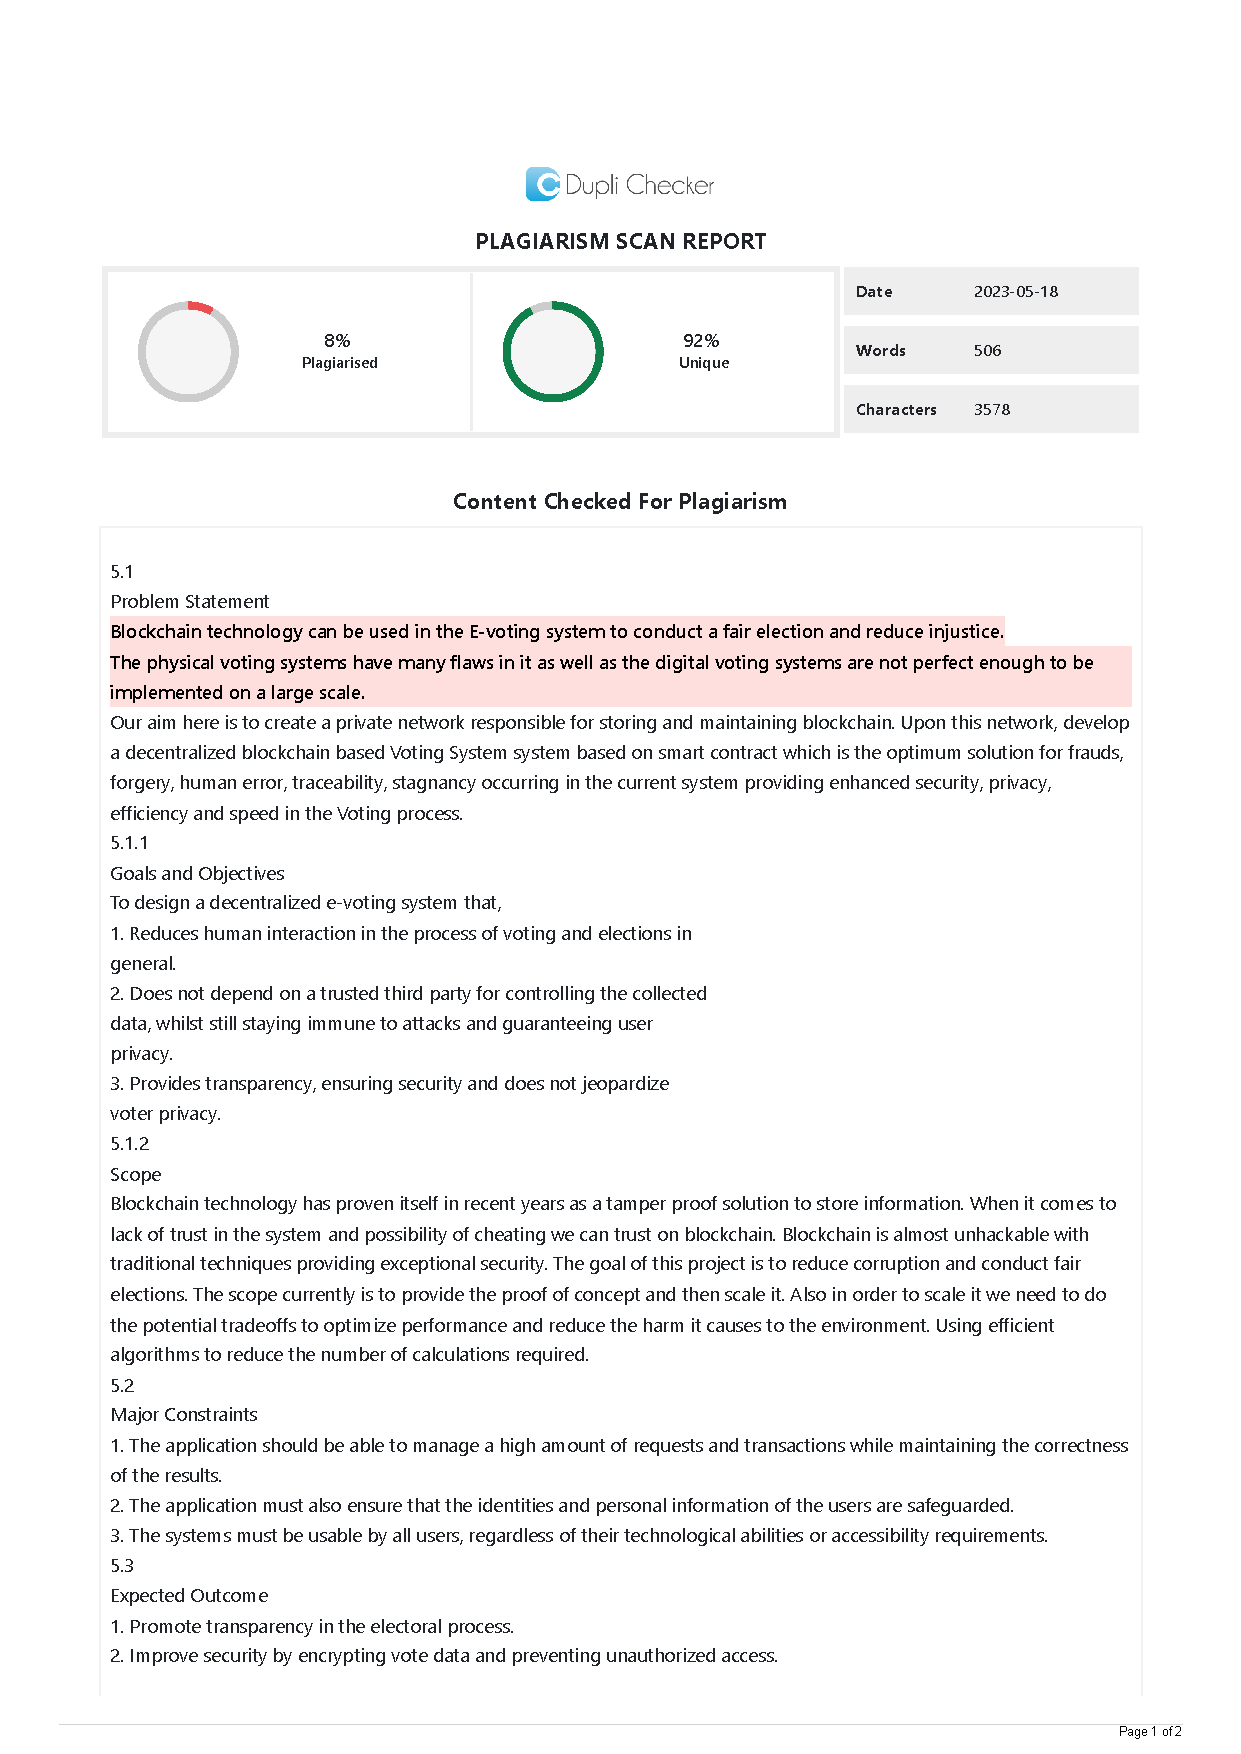
\includepdf[pages=-]{./Resources/plagiarism-report.pdf}
\newpage
\section{Annexure D:\\Term II - Project Laboratory Assignments}
\newpage
\subsection{Coverage report}
\colorbox{gray!20}{%
	\begin{minipage}{\linewidth}%
		\vspace*{2pt}
		\textbf{Version}
		\\\textbf{=======}
		\\$>$ \textbf{solidity-coverage:} v0.8.2
			\\\\\textbf{Instrumenting for coverage...}
			\\\textbf{=============================}
			\\\\$>$ ElectoralContract.sol
		\\\\\textbf{Compilation:}
		\\\textbf{============}
		\\\\Compiled 1 Solidity file successfully
		\\\\\textbf{Network Info}
		\\\textbf{============}
		\\$>$ \textbf{HardhatEVM:} v2.14.0
			\\$>$ \textbf{network:}    hardhat
		\\\\\\ElectoralContract
		\begin{itemize}
			\item[\checkmark] Should add candidates and voters on deployment (279ms)
			\item[\checkmark] Should add candidate (85ms)
			\item[\checkmark] Should add voter
			\item[\checkmark] Should login and logout (43ms)
			\item[\checkmark] Should cast vote (88ms)
		\end{itemize}
		5 passing (534ms)
		\begin{table}[H]
			\resizebox{0.97\textwidth}{!}{%
				\begin{tabular}{|l|r|r|r|r|l|}
					\hline
					File                                                                      & \multicolumn{1}{l|}{\% Stmts}                     & \multicolumn{1}{l|}{\% Branch}                  & \multicolumn{1}{l|}{\% Funcs}                     & \multicolumn{1}{l|}{\% Lines}                     & Uncovered Lines \\ \hline
					\begin{tabular}[c]{@{}l@{}}contracts/\\ElectoralContract.sol\end{tabular} & \begin{tabular}[c]{@{}r@{}}100\\ 100\end{tabular} & \begin{tabular}[c]{@{}r@{}}50\\ 50\end{tabular} & \begin{tabular}[c]{@{}r@{}}100\\ 100\end{tabular} & \begin{tabular}[c]{@{}r@{}}100\\ 100\end{tabular} &                 \\ \hline
					All files                                                                 & 100                                               & 50                                              & 100                                               & 100                                               &                 \\ \hline
				\end{tabular}%
			}
		\end{table}
		\vspace*{2pt}
	\end{minipage}%
}
\subsection{Test report}
\colorbox{gray!20}{%
	\begin{minipage}{\linewidth}%
		\vspace*{2pt}
		Compiled 1 Solidity file successfully
		\\\\ ElectoralContract
		\begin{itemize}
			\item[\checkmark] Should add candidates and voters on deployment
			\item[\checkmark] Should add candidate
			\item[\checkmark] Should add voter
			\item[\checkmark] Should login and logout
			\item[\checkmark] Should cast vote
		\end{itemize}
		\begin{table}[H]
			\resizebox{0.97\textwidth}{!}{%
				\begin{tabular}{|ll|lllll|}
					\hline
					\multicolumn{2}{|l|}{Solc version: 0.8.19} & \multicolumn{2}{l|}{Optimizer enabled: false} & \multicolumn{1}{l|}{Runs: 200}   & \multicolumn{2}{l|}{Block limit: 30000000 gas}                                                                                             \\ \hline
					\multicolumn{2}{|l|}{Methods}              & \multicolumn{5}{l|}{}                                                                                                                                                                                                         \\ \hline
					\multicolumn{1}{|l|}{\textbf{Contract}}    & \textbf{Contract}                             & \multicolumn{1}{l|}{Min}         & \multicolumn{1}{l|}{Max}                       & \multicolumn{1}{l|}{Avg}    & \multicolumn{1}{l|}{\textbf{\# calls}} & \textbf{usd (avg)} \\ \hline
					\multicolumn{1}{|l|}{ElectoralContract}    & addCandidate                                  & \multicolumn{1}{l|}{-}           & \multicolumn{1}{l|}{-}                         & \multicolumn{1}{l|}{114760} & \multicolumn{1}{l|}{2}                 & -                  \\ \hline
					\multicolumn{1}{|l|}{ElectoralContract}    & addVoter                                      & \multicolumn{1}{l|}{-}           & \multicolumn{1}{l|}{-}                         & \multicolumn{1}{l|}{143693} & \multicolumn{1}{l|}{3}                 & -                  \\ \hline
					\multicolumn{1}{|l|}{ElectoralContract}    & login                                         & \multicolumn{1}{l|}{-}           & \multicolumn{1}{l|}{-}                         & \multicolumn{1}{l|}{51926}  & \multicolumn{1}{l|}{2}                 & -                  \\ \hline
					\multicolumn{1}{|l|}{ElectoralContract}    & logout                                        & \multicolumn{1}{l|}{-}           & \multicolumn{1}{l|}{-}                         & \multicolumn{1}{l|}{24557}  & \multicolumn{1}{l|}{1}                 & -                  \\ \hline
					\multicolumn{1}{|l|}{ElectoralContract}    & vote                                          & \multicolumn{1}{l|}{-}           & \multicolumn{1}{l|}{-}                         & \multicolumn{1}{l|}{80429}  & \multicolumn{1}{l|}{1}                 & -                  \\ \hline
					\multicolumn{2}{|l|}{Deployments}          & \multicolumn{3}{l|}{}                         & \multicolumn{1}{l|}{\% of limit} &                                                                                                                                            \\ \hline
					\multicolumn{2}{|l|}{ElectoralContract}    & \multicolumn{1}{l|}{1578809}                  & \multicolumn{1}{l|}{1924953}     & \multicolumn{1}{l|}{1751881}                   & \multicolumn{1}{l|}{5.8 \%} & -                                                           \\ \hline
				\end{tabular}%
			}
		\end{table}
		5 passing (1s)
		\vspace*{2pt}
	\end{minipage}%
}
\newpage
\section{Annexure E:\\Publications}
\newpage
\subsection{Survey Paper}
\subsubsection{Title}
Survey on Blockchain Technology and its application in Electoral Voting System
\subsubsection{Journal}
International Journal for Research in Applied Science \& Engineering Technology (IJRASET)
\subsubsection{Volume}
10
\subsubsection{Issue}
XI
\subsubsection{Month of Publication}
November 2022
\subsubsection{Digital Object Identifier (DOI)}
\href{https://doi.org/10.22214/ijraset.2022.47752}{https://doi.org/10.22214/ijraset.2022.47752}
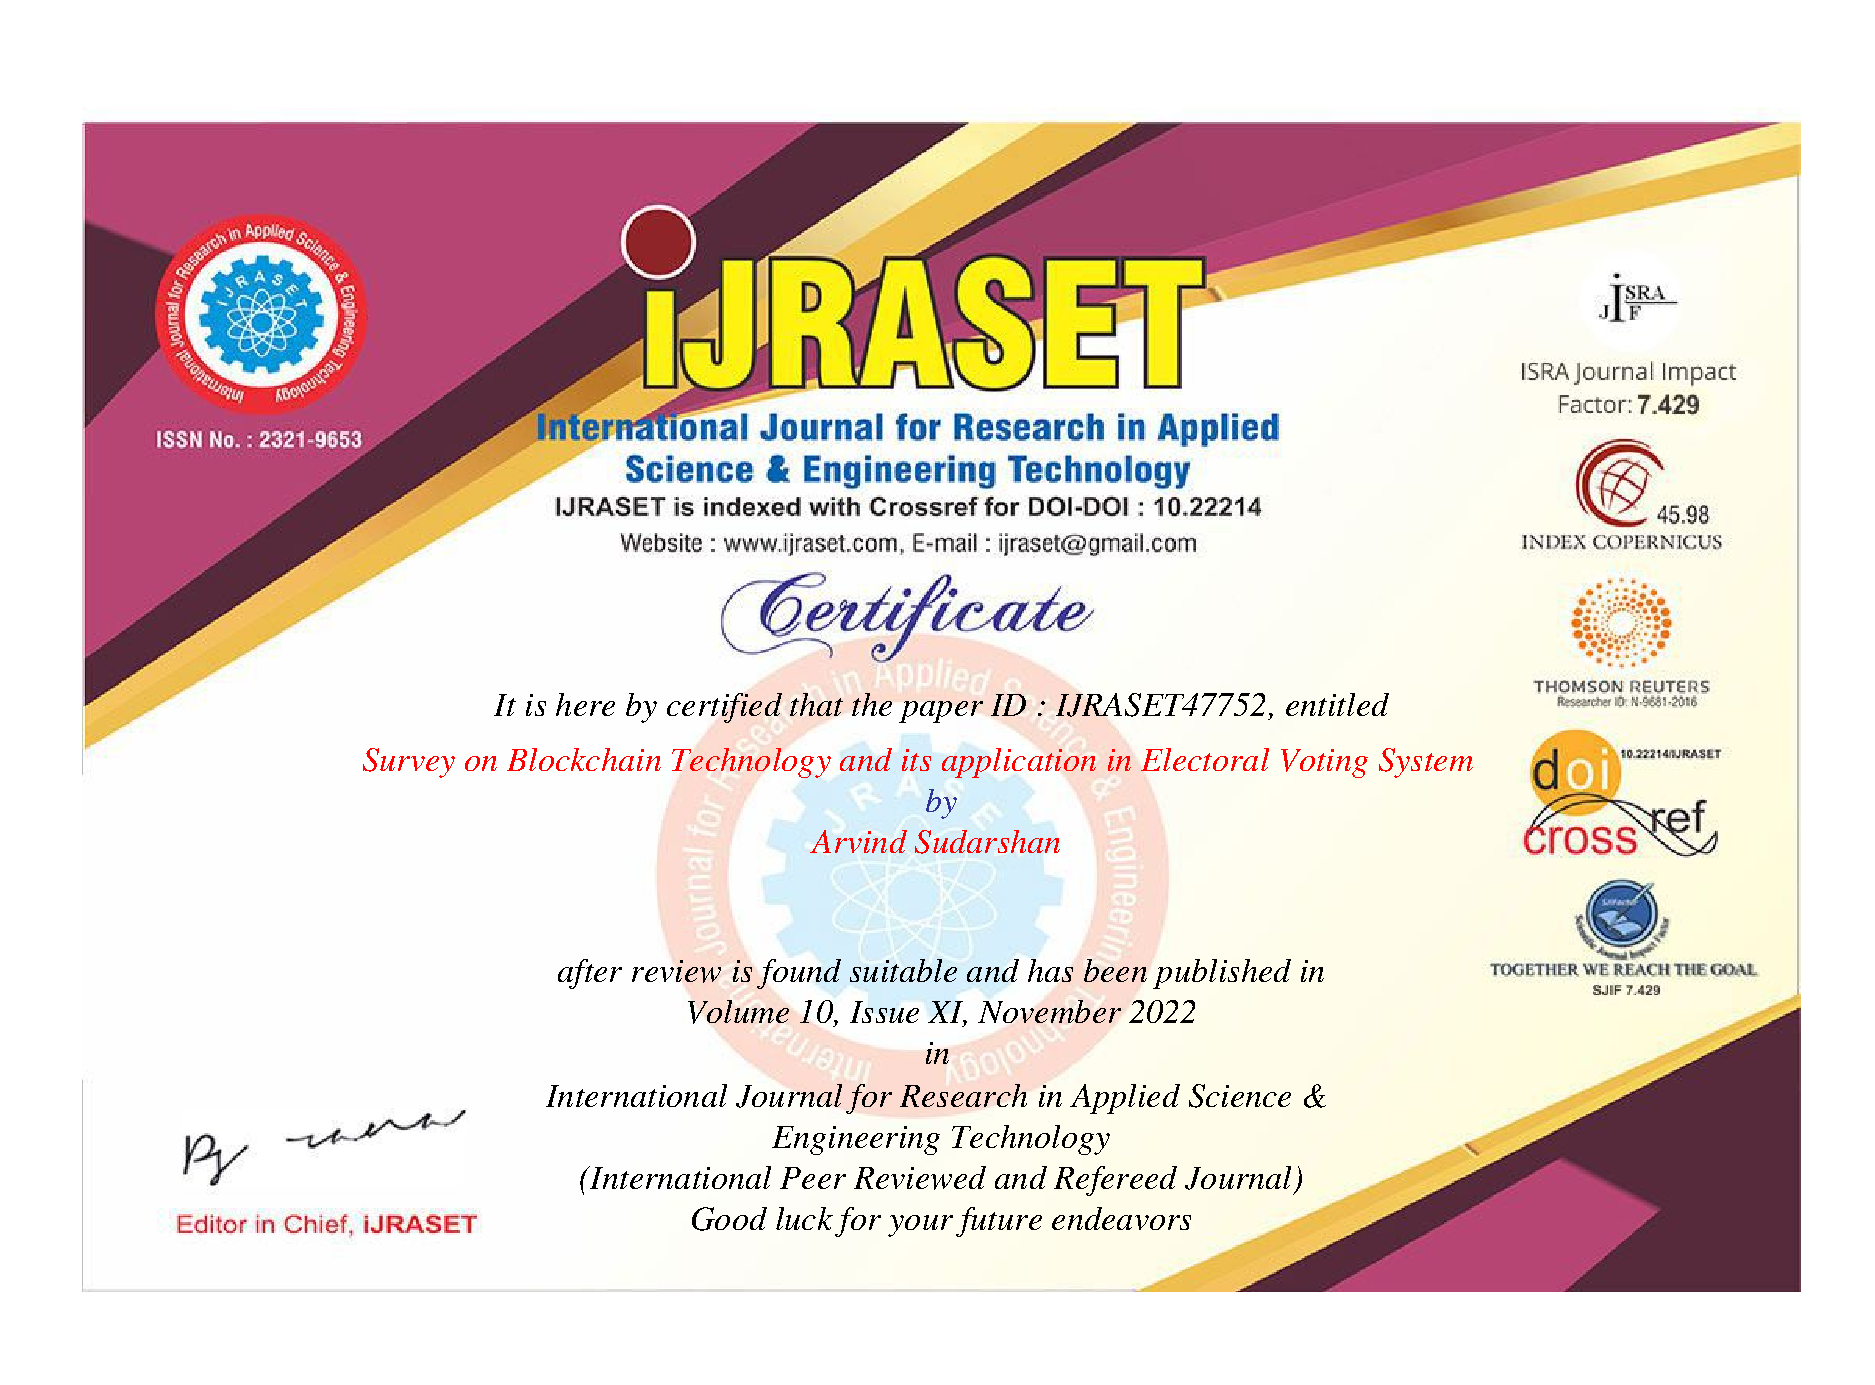
\includepdf[pages=-,nup=1x2]{./Resources/IJRASET-certificates.pdf}
\newpage
\section{Annexure F:\\Competitions}
\newpage
\subsection{Project Competition}
\subsubsection{Event}
Project Competition 2K23\\5th May, 2023
\subsubsection{Organizer}
Pune Vidhyarthi Griha’s College of Engineering and Technology and G. K. Pate (Wani) Institute of Management
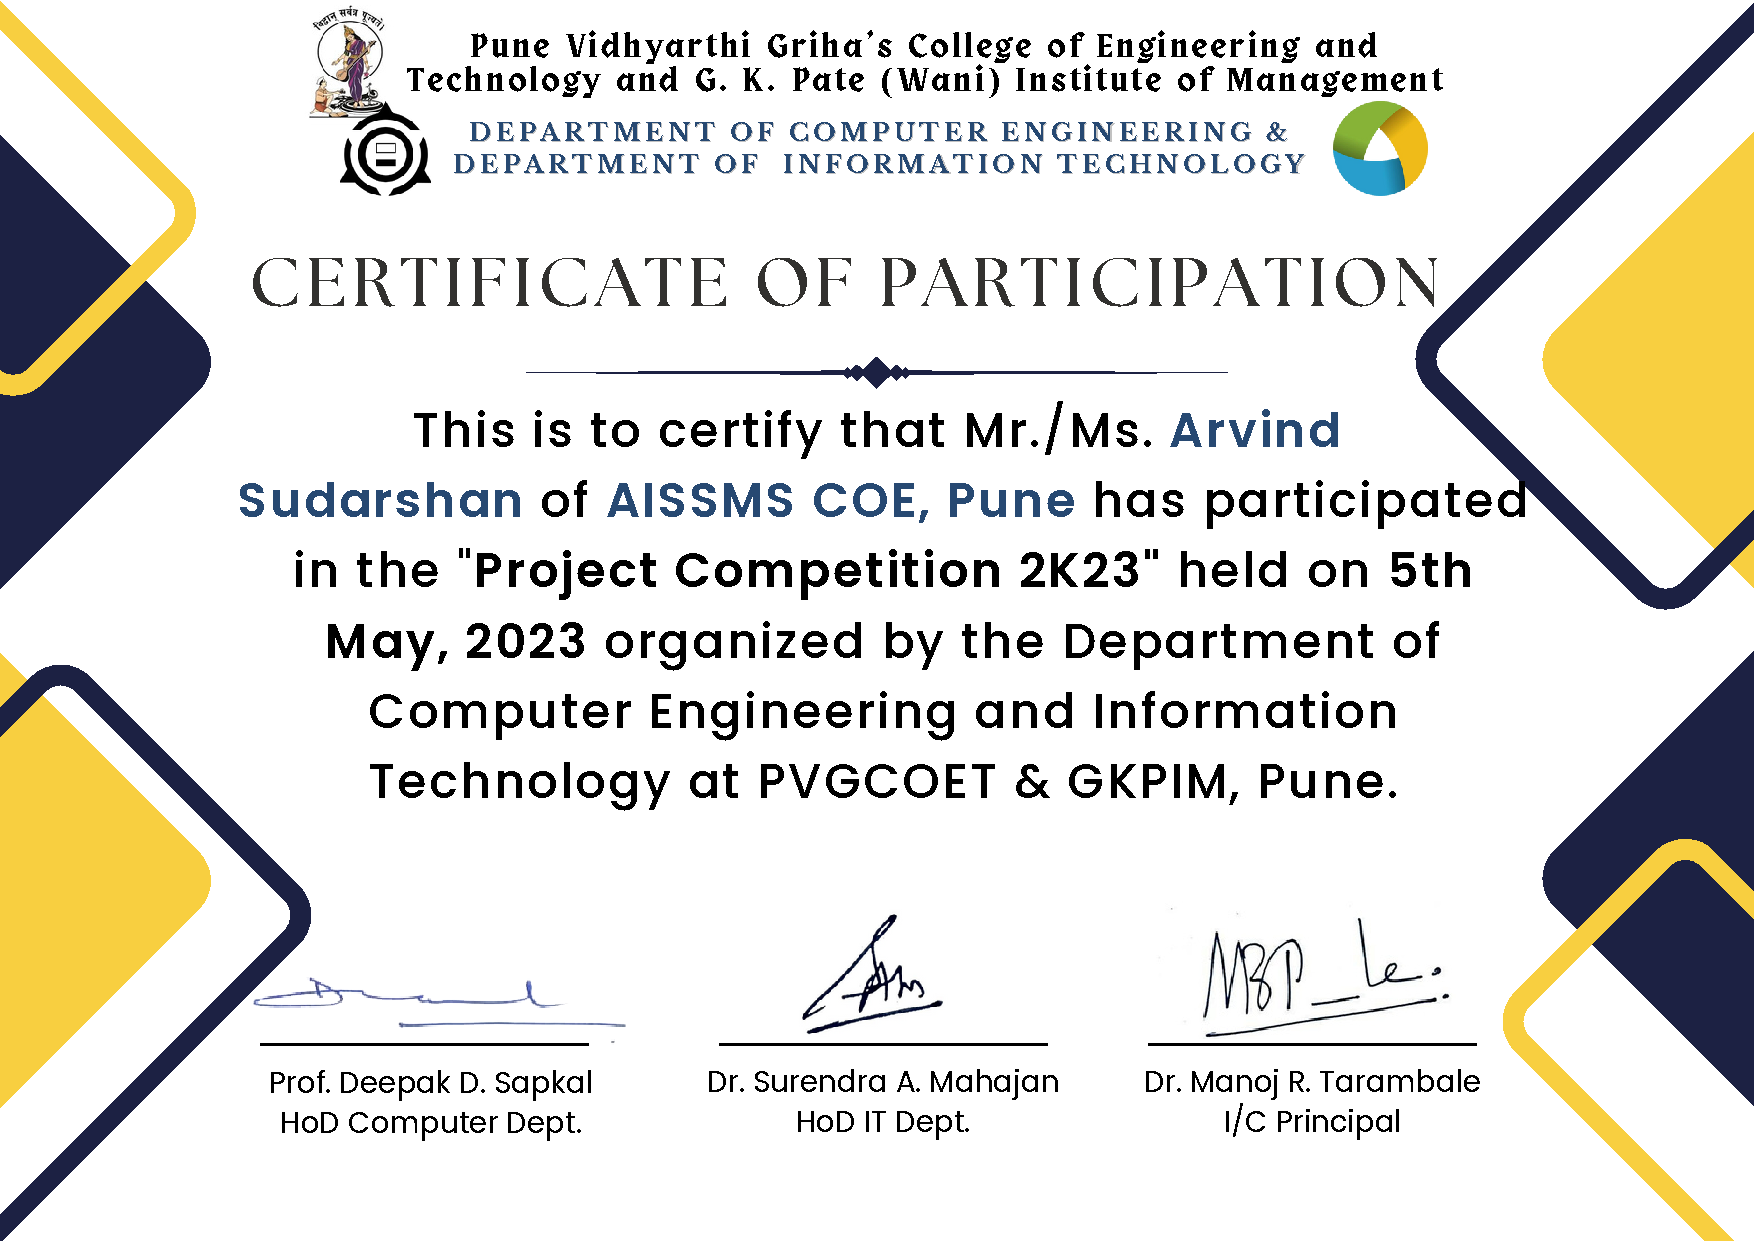
\includepdf[pages=-,nup=1x2,delta=0in 0.5in,offset=0in 0.25in,scale=0.9]{./Resources/PVG-certificates.pdf}
\newpage
\section{Annexure G:\\Information of Project Group Members}
\newpage
\begin{table}[H]
	\begin{tabular*}{\textwidth}{lll@{\extracolsep{\fill}}l}
		Name        & : & Arvind Sudarshan            & \multirow{6}{*}{\fbox{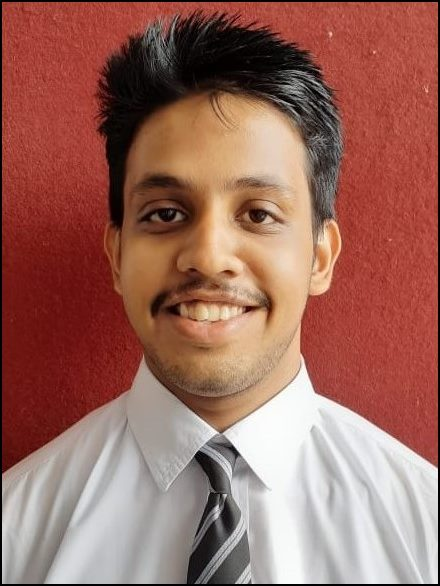
\includegraphics[height=1.5in]{./Resources/arvind.jpg}}} \\\\
		DOB         & : & August 19, 2001             &                   \\\\
		Gender      & : & Male                        &                   \\\\
		Address     & : & Pune, Maharashtra           &                   \\\\
		Email       & : & arvindsudarshan18@gmail.com &                   \\\\\\\\

		Name        & : & Chatane Shree Atul 		  & \multirow{6}{*}{\fbox{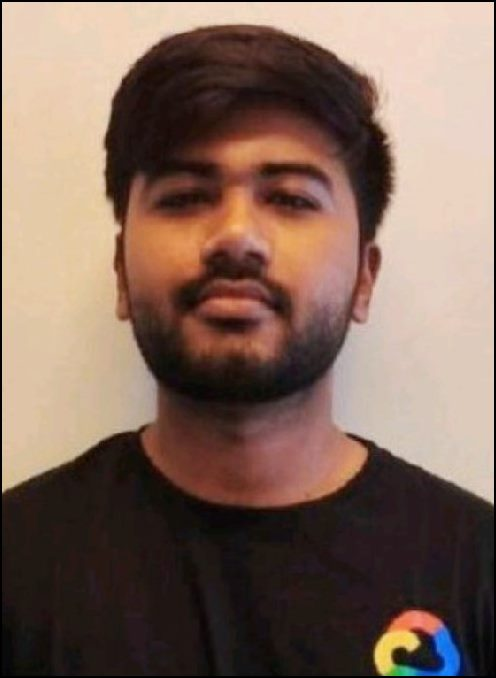
\includegraphics[height=1.5in]{./Resources/shree.jpg}}} \\\\
		DOB         & : & October 3, 2001			  &                   \\\\
		Gender      & : & Male                 		  &                   \\\\
		Address     & : & Pune, Maharashtra    		  &                   \\\\
		Email       & : & shreeameyc@gmail.com 		  &                   \\\\\\\\

		Name        & : & Eksambekar Yash Sagar    	  & \multirow{6}{*}{\fbox{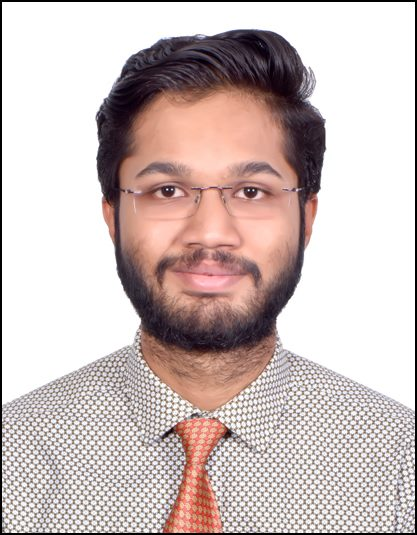
\includegraphics[height=1.5in]{./Resources/yash.jpg}}} \\\\
		DOB         & : & July 16, 2001            	  &                   \\\\
		Gender      & : & Male                     	  &                   \\\\
		Address     & : & Pune, Maharashtra        	  &                   \\\\
		Email       & : & yasheksambekar@gmail.com 	  &                   \\\\\\\\

		Name        & : & Gadkari Gaurav Sudhir        & \multirow{6}{*}{\fbox{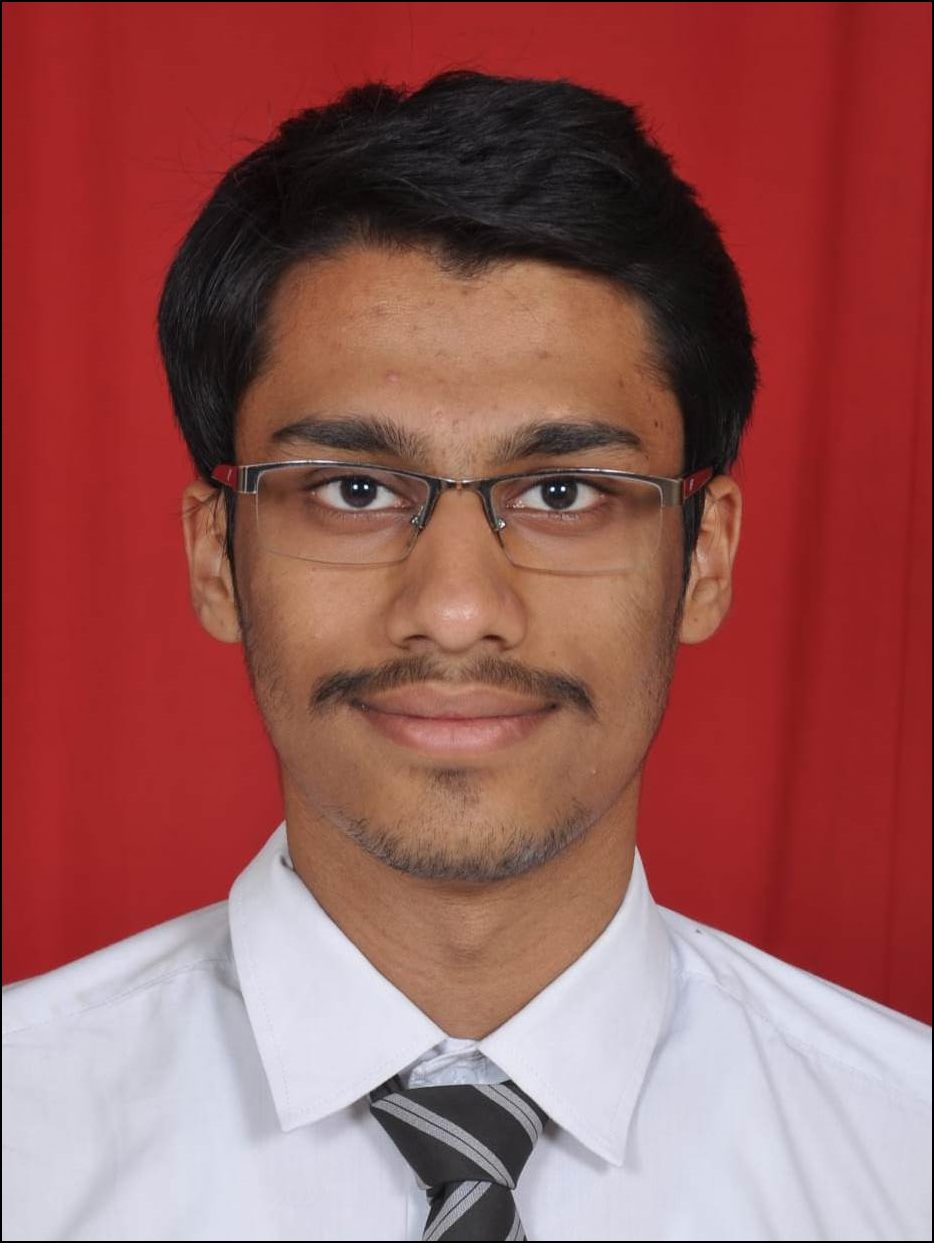
\includegraphics[height=1.5in]{./Resources/gaurav.jpg}}} \\\\
		DOB         & : & August 19, 2001              &                   \\\\
		Gender      & : & Male                         &                   \\\\
		Address     & : & Pune, Maharashtra            &                   \\\\
		Email       & : & gaurav.gadkari1908@gmail.com &                   \\\\
	\end{tabular*}
\end{table}
\end{document}
